 \documentclass{article}

% From last round: 

% Marcus playing with page layout

% Marcus, that's generally a bad idea. It's almost always wrong
% to make the page too wide; there is a good reason why e.g. newspaper
% articles are usually set in one narrow header and two even narrower
% columns underneath. The reason is that the eye loses position
% jumping back left to the beginning of the line if the right
% edge is out of view.
% We should first see how it comes out. 

% Marty, the standard margins are too wide in the default article documentclass.  
% The settings below create the standard 1-inch margins all around. Reinstating...

% This round:

%Marty, if you have a smoother way of achieving standard 1-inch margins in a letter-size document, please implement. For now, this is working

\oddsidemargin=0in
\evensidemargin=0in

%\addtolength{\textwidth}{0.16\textwidth}
\textwidth=6.5in % please leave this in place as is - thanks, Marcus
\textheight=9in
\topmargin=0in
\headheight=0in
\headsep=0in
\footskip=0.5in

%
\usepackage[utf8]{inputenc}
\usepackage{enumitem,kantlipsum}
\usepackage[style=numeric,sorting=none]{biblatex}

%
%%%%%% ``Header'' with a collection of useful definitions  

\RequirePackage{lineno}

\usepackage{graphicx}
%\DeclareGraphicsExtensions{.pdf,.png,.jpg}

\usepackage{url}
\usepackage{hyperref}
\hypersetup{colorlinks=true, linkcolor=black, urlcolor=cyan}

\usepackage{xspace}

\newcommand{\filenamedot}{.}
\setlength{\parindent}{0.0in}
\setlength{\parskip}{0.1in}
\renewcommand{\topfraction} {0.9}
\renewcommand{\bottomfraction} {0.9}
\renewcommand{\textfraction} {0.1}
\renewcommand{\floatpagefraction} {0.8}

%\usepackage{fancyhdr}
%\pagestyle{fancy}

\usepackage{eurosym}
\usepackage{xcolor}
\usepackage{siunitx}

\newcommand{\hic}{\mbox{$A$$+$$A$}\xspace}
\newcommand{\pA}{\mbox{$p$$+$$A$}\xspace}
\newcommand{\AuAu}{\mbox{Au$+$Au}\xspace}
\newcommand{\auau}{\mbox{Au$+$Au}\xspace} 
\newcommand{\raa}{\mbox{$R_\mathrm{AA}$}\xspace}
\newcommand{\pbpb}{\mbox{Pb$+$Pb}\xspace} 
\newcommand{\pdau}{\mbox{$p(d)$$+$Au}\xspace} 
\newcommand{\pau}{\mbox{$p$$+$Au}\xspace} 
\newcommand{\aj}{\mbox{$A_J$}\xspace} 
\newcommand {\pp}{\mbox{$p$$+$$p$}\xspace}
\newcommand {\ppbar}{\mbox{$p$$+$$\overline{p}$}\xspace}
\newcommand{\pT}{\mbox{${p_T}$}\xspace}
\newcommand{\jpsi}{\mbox{$J/\psi$}}
\newcommand{\sqrtsnn}{\mbox{$\sqrt{s_{\scriptscriptstyle NN}}$}}
\newcommand{\npart}{$N_\mathrm{part}$}
\newcommand{\ncoll}{$N_\mathrm{coll}$}
\newcommand{\qgp}{\mbox{quark-gluon plasma}\xspace}
\newcommand{\jt}{\mbox{$J_T$}} \newcommand{\qhat}{\mbox{$\hat{q}$}}
\newcommand{\Qsqr}{\mbox{$Q^2$}} \newcommand{\CuCu}{\mbox{Cu$+$Cu}}
\newcommand{\PbPb}{\mbox{Pb$+$Pb}} \newcommand{\pPb}{\mbox{$p$$+$Pb}}
\newcommand{\gjet}{\mbox{$\gamma$-jet}}
\newcommand{\Qmax}{\mbox{$Q_{\max}$}} \newcommand{\ET}{\mbox{$E_T$}}
\newcommand{\Et}{\mbox{$E_T$}} \newcommand{\kt}{\mbox{$k_T$}}
\newcommand{\RAA}{\mbox{$R_{AA}$}\xspace} \newcommand{\IAA}{\mbox{$I_{AA}$}}
\newcommand{\pt}{\mbox{${p_T}$}\xspace}
\newcommand{\highpt}{high-${\rm p_{_{T}}}$}
\newcommand{\lessim}{{\stackrel{<}{\sim}}} \newcommand{\eqnpt}{p_T}
\newcommand{\eA}{\mbox{$e-{\rm A}$}}
\newcommand{\dAu}{\mbox{$d$$+$Au}\xspace}
\newcommand{\pAu}{\mbox{$p$$+$Au}\xspace}
\newcommand{\GeVSQ}{\mbox{${\rm GeV}^2$}}
\newcommand{\fastjet}{\mbox{\sc FastJet}\xspace}
\newcommand{\geant}{\mbox{\sc Geant4}\xspace}
\newcommand{\pizero}{\mbox{$\pi^0$}\xspace}

\newcommand{\red}{\color{red}}
\newcommand{\blue}{\color{blue}}	 
\newcommand{\green}{\color{green}}	 
\newcommand{\magenta}{\color{magenta}}

\newcommand{\lyxdot}{.}
%\usepackage{subfig}




\addbibresource{BNL.bib}
\addbibresource{FIT.bib}
\addbibresource{INFN.bib}  
\addbibresource{SBU.bib}
\addbibresource{UVa.bib}
\addbibresource{Yale.bib}
\addbibresource{TU.bib}

\begin{document}
%
%\input{eRD6_consortium}
\title{\bf EIC Detector R\&D Progress Report}
\author{The EIC Tracking and PID Consortium \vspace*{1mm}\\ (eRD6 Consortium)}
\maketitle
%
%\begin{center}
%\section*{\centering{eRD6 R\&D Progress Report}}
%\end{center}

\subsection*{The eRD6 Consortium} 
\begin{itemize}
\item[] {\bf Project ID:} eRD6
\item[] {\bf Project Name:} Tracking \& PID detector R\&D towards an EIC detector
\item[]{\bf Period Reported:} From July 2018 to December 2018
\item[]{\bf Project Leaders:}
%
\begin{itemize}
\item[] Brookhaven National Lab (BNL): Craig Woody
\item[] Florida Institute of Technology (FIT): Marcus Hohlmann
\item[] INFN Trieste: Silvia Dalla Torre
\item[] Stony Brook University (SBU): Klaus Dehmelt, Thomas Hemmick
\item[] Temple University (TU): Matt Posik, Bernd Surrow
\item[] University of Virginia (UVa): Kondo Gnanvo, Nilanga Liyanage
\item[] Yale University: Richard Majka, Nikolai Smirnov
\end{itemize}
%
\item[]{\bf Project Members:}
%
\begin{itemize}
\item[] BNL: B. Azmoun, A. Kiselev, M. L. Purschke, C. Woody
\item[] BNL - Medium Energy Group: E. C. Aschenauer
\item[] FIT: M. Bomberger, M. Hohlmann
\item[] INFN Trieste: S. Dalla Torre, S. Levorato, F. Tessarotto
\item[] SBU: K. Dehmelt, A. Deshpande, P. Garg, T. K. Hemmick
\item[] TU: M. Posik, A. Quintero, B. Surrow
\item[] UVa: K. Gnanvo, N. Liyanage
\item[] Yale University: R. Majka, N. Smirnov
\end{itemize}
%
\item[]{\bf Contact Person:} Kondo Gnanvo; \href{mailto:kgnanvo@virginia.edu}{kgnanvo@virginia.edu}
%
\end{itemize}

\newpage
\tableofcontents

\renewcommand{\baselinestretch}{1.02}
\newpage
%
\section{Past}
\subsection{Brief overview of project histories}
\subsubsection{Brookhaven National Lab} 
The group at BNL is mainly engaged in optimizing micro-pattern gaseous detectors (MPGD’s) for reading out a time projection chamber (TPC) for use at the EIC. 

Over the last few years we have built and tested numerous planar GEM detectors with long (\textasciitilde16mm) and short (\textasciitilde3mm) drift regions and have equipped them with both zigzag pad and strip readout geometries in an effort to study the spatial and angular resolution of a host of detector configurations. Following detailed studies of these detectors in the lab, beam tests were also carried out in 2012 and 2104 at Fermilab to fully characterize the performance of GEM detectors with extended drift gaps under beam conditions. The results of these efforts were published in a peer reviewed journal in 2014\cite{7497629}.

In addition, in collaboration with Stony Brook U. and Yale U., we have built a prototype combination TPC-Cherenkov (TPCC) detector to study the feasibility of performing tracking and pID measurements in a common detector volume. The detector was filled with a specially chosen gas to be used as both the Cherenkov radiator and the TPC working gas. After investigating important characteristics such as the drift velocity and the charge spread in various candidate gases, a beam test was conducted to demonstrate a proof of principle of the viability of this detector concept. The results from these tests were positive and are detailed in a recently completed manuscript that will be submitted very shortly to a peer review journal (IEEE TNS) for publication. (Preliminary results from the TPCC have also already been presented at several conferences and have appeared in various conference proceedings\cite{Woody:2015ola}.)

More recently we have focused on optimizing the design of the readout plane for a GEM detector made of zigzag shaped charge collecting anodes. We initially performed simulations to study the zigzag geometry, followed by a systematic set of measurements in the lab to reveal which geometrical parameters drive the performance of the readout. The results of these investigations were recently published in a peer review journal \cite{8379440}, with collaborators from Florida Tech and Stony Brook U. We have continued to refine the design of the zigzag readout by pushing the design parameters beyond what could be produced using standard chemical etching processes. A novel laser etching technique was used to generate PCB’s with zigzag pad geometries with significantly finer features that more closely resemble idealized patterns determined by simulation. These new PCB’s were also tested in the lab and very recently at a beam test at FNAL. A summary of these investigations was recently submitted to the 2018 IEEE NSS conference for consideration. 

Now that our work with optimizing the zigzag pads is complete, our focus is primarily aimed at investigating various avalanche technologies for a TPC readout including GEM’s, Micromegas, a combinations of the two, and $\mu$RWELL. 


\subsubsection{Florida Tech} 
The Florida Tech group has been focusing on the development of large low-mass GEM detectors with low channel count for the forward tracker (FT) of the EIC detector. In the current funding cycle the group has begun shifting focus towards R\&D on cylindrical $\boldmath{\mu}$RWELL detectors for a fast central tracker at an EIC detector.

We initially designed and implemented radial zigzag strips on large readout PCBs to achieve low-channel count while maintaining good spatial resolution. We constructed a first one-meter-long prototype with such a readout at Florida Tech using a purely mechanical construction technique without any gluing and tested it in beams at Fermilab in 2013. This study showed a non-linearity in the position measurement of hits\cite{Zhang:2015pqa}. The reason was an over-etching of tips and under-etching of troughs in the zigzag strips, which caused insufficient interleaving of adjacent strips and consequently insufficient charge sharing among strips. We adjusted the zigzag strip design to improve the strip interleaving. Small PCBs and a flex-foil with the improved zigzag strip design were produced by industry and by CERN, respectively. We subsequently tested these with highly collimated X-rays at BNL. A substantial reduction in the non-linearity and an improvement in spatial resolution were observed\cite{Zhang:2017dqw}.

Next, we designed a second large Triple-GEM detector that implements the drift electrode and a readout electrode with improved radial zigzag strips on polyimide foils rather than on PCBs to reduce the material in the active detector area\cite{Hohlmann:2017sqj}. These foils were then produced by CERN. To provide sufficient rigidity to this new detector while maintaining low mass, we produced the main support frames from carbon fiber material. We designed the GEM foils for this second detector in such a way that they can also be used for the second UVa FT prototype (``common GEM foil design''). A number of these GEM foil were produced for Florida Tech and UVa by the CERN workshop using the single-mask foil etching technique. Assembly of this second prototype showed that 3D-printed pull-out and frame components made from ABS did not have sufficient material strength to sustain the mechanical forces needed for stretching. They are now being replaced by stronger components made from PEEK.
\subsubsection{INFN Trieste} 
The task of the INFN participants to the eRD6 
Consortium is 
"Further development of hybrid MPGDs for single photon 
detection synergistic to TPC read-out sensors".
\par
Particle identification of electrons and hadrons
over a wide momentum range is a key ingredient 
for the physics programme at EIC. One of the most
challenging aspects is hadron identification at
high momenta, namely above 6-8~GeV/c, where the
only possibility is the use of Cherenkov imaging
techniques with gaseous radiator. The overall
constrains of the experimental set-ups at a
collider impose a limited RICH detector length 
and to operate in magnetic fringing field. 
The use, for this RICH,  
of gaseous photon detectors is 
one of the 
most likely choice. The goal of our project 
is an R\&D to further develop MPGD-based single photon
detectors in order to establish 
one of the key components of the RICH for high momentum
hadrons. This R\&D has also 
some aspects synergistic to the development 
of TPC sensors: the miniaturization of the 
read-out elements and the reduction of the 
Ions Back-Flow (IBF). 
\par
The starting point are the hybrid MPGD detectors
of single photons developed for the upgrade of 
the gaseous RICH 
counter~\cite{ALBRECHT2005215,
ABBON2008371,ABBON201021,
ABBON201126} of the COMPASS 
experiment~\cite{ABBON2007455,ABBON201569} 
at CERN SPS. These detectors are the result of 
several years of dedicated 
R\&D~\cites{ALEXEEV2009174,
ALEXEEV2010396,ALEXEEV2010129,
Alexeev:2012tba,
1748-0221-5-03-P03009,ALEXEEV2011130,ALEXEEV2012159,
1748-0221-7-02-C02014,
Alexeev:2012rva,ALEXEEV2013264,
1748-0221-8-12-C12005,
1748-0221-8-01-P01021,
ALEXEEV2014133,1748-0221-9-03-C03046,
1748-0221-9-09-C09017,
Levorato:2014gya,1748-0221-10-03-P03026,
ALEXEEV2016139,2017233}. 
They
consists in three
multiplication stages:
two THick GEMs (THGEM) layers, the first one
coated with a CsI film and acting as 
photocathode, followed by a resistive MicroMegas (MM)
multiplication stage. The COMPASS photon detectors 
can operate at gains of at least~3$\times$10$^4$
and exhibit an IBF rate lower 
than~5\%~\cite{ALEXEEV2016139,
ALEXEEV201796,1748-0221-12-07-C07026,AGARWALA2017,
AGARWALA2018}. 
An original element of
the hybrid MPGD photon detector is the approach
to a resistive MM by discrete elements:
the anode pads
facing the micromesh are
individually equipped with large-value resistors
and the HV is provided, via these resistors, to
the anode electrodes, while the micromesh is
grounded. A second set of electrodes (pads
parallel to the first ones) are embedded in the
anode PCB: the signal is transferred by 
capacitive coupling to these electrodes, 
which are connected to the front-end 
read-out electronics.
\par
The whole R\&D project develops over several years 
and it includes
further improvements of the hybrid MPGD-based photon 
detectors in order to match the requirements of high 
momenta hadron identification at EIC and initial tests
relative to  the application in gaseous detectors of a 
novel photocathode concept, based on NanoDiamond (ND) 
particles~\cite{VELARDI20171}.
\subsubsection{Stony Brook University} 
SBU is concentrating on the study of Ion Backflow (IBF) for a TPC, a possible candidate for the central tracker in at least one of the EIC detectors for an EIC. Furthermore, the TPC for sPHENIX has the same physical size when used in, e.g., the BeAST EIC detector. 

It has been shown that IBF will pose a problem in an EIC detector and that the ultimate EIC TPC device must do more than sPHENIX to achieve the same level of position distortion. Our approach is to investigate new structures in and around the multiplication stage that promise significant better performance when considering IBF.

SBU proposed in the latest funding cycle the investigation of a new detector concept that might allow to significantly enhance particle identification via the Cherenkov effect with the help of meta-materials.

SBU also is working on the final installation of a unit that allows to produce high quality large size mirrors for RICH applications. The project is ongoing and expected to be finalized in about two months.
\subsubsection{Temple University} 
Temple University (TU) has been focusing mainly on completing the the assembly and characterization of the commercial triple-GEM detectors. This R\&D work was carried over from the eRD3 + eRD6 merger. These commercial triple-GEM detectors follow the STAR FGT triple-GEM design~\cite{STARfgt}, but use commercial GEM, HV, and readout foils that were produced by Tech-Etch. Additionally these detectors are investigating the use of Kapton spacer rings in place of the more traditional G10 spacer grids. We were able to identify the cause of the electrical short that led to excessive sparking in the first two commercial triple-GEM detectors that were built last summer. Using the remaining materials, we are able to build two more commercial triple-GEM detectors prototypes 3 and 4. The third detector has now been completely assembled and is undergoing characterization, while the all foils for the fourth commercial triple-GEM have been glued and stretched. During the third and fourth detector assemblies we implemented a fix to prevent the same shorting that occurred in the first two triple-GEM detectors. This fix was verified with the third chamber that we built.

In addition to finishing out the commercial triple-GEM work, we are beginning to focus on some simulation work. In particular the use of an MPGD in $\mu$TPC mode as a replacement or in addition to a TPC. This detector simulation work is being done to see if it would be practical to use such a detector in a second EIC detector stack located at another IR location. We now have the basic machinery in place which enables us to easily adjust the dead material, gas, drift gap size, number of hit points, and specify the hit point, radial, and transverse resolutions of the detector. Work has now just started to modify these parameters to simulate a realistic detector digitization. To determine the proper resolution parameters test beam data taken by BNL with a MPGD operating in $\mu$TPC mode using a COMPASS styled readout. Ultimately this simulation work of the $\mu$TPC will be integrated into the simulation work that is being done at FIT relating to the forward MPGD tracking. This integration will allow for a full tracking simulation which covers the mid-rapidity region consisting of a vertex detector and a MPGD $\mu$TPC barrel detector, as well as the forward/backward regions consisting of tracking MPGD detectors.
\subsubsection{University of Virginia} 
The focus of the group at UVa is the development of high performance, large and low mass GEM detector  for the forward region of an EIC detector. 

Our R\&D  at UVa shares some similarities with the development by the Florida Tech group and by Temple U. group within the eRD3 program but we are specifically focused on the development of high performance, large area two dimensional U-V strip readout with fine pitch to provide excellent spatial resolution in both radial and azimuthal direction. A first prototype of such detector was built and successfully tested at the Fermilab Test Beam Facility (FTBF) in 2013. The analysis of the test beam data fully validated the expected performances of the U-V strip readout and the results were published in \cite{Gnanvo:2015xda}. 

We  recently completed the second phase of the R\&D with a design improvement of the U-V strip readout to push even further the spatial resolution capabilities in both dimensions. The new prototype is conceived around the "Common EIC GEM foil design" jointly developed by UVa, Florida Tech (FIT)  and Temple University (TU) groups of the eRD6 consortium. We have also been testing new ideas such as the ultra low mass Chromium GEM foil to reduce even further the material budget of EIC-FT GEM detectors and the development of the double-sided zebra connection scheme to provide an elegant solution for the fine pitch U-V strip readout layer. We anticipate that several of these innovative ideas will ultimately be integrated in the final design of the large area EIC  forward GEM trackers.

We are also conducting in collaboration with TU and FIT, some R\&D on a new MPGD detector technology, the $\mu$RWELL device, that we view as an alternative to GEM or Micromegas and an ideal candidate for cylindrical tracking device in the barrel region of the EIC detector. 


\subsubsection{Yale University} 


\subsection{What was planned for this period?} 
\subsubsection{Brookhaven National Lab}

\begin{enumerate}

\item	\textbf{\emph{TPC prototype}}: We planned to complete the assembly and commissioning of our new TPC prototype detector, which reuses the 10cm x 10cm x 10cm field cage from our older TPCC prototype detector. Ultimately, we plan to use this prototype to study various readout plane geometries (including zigzag shaped charge collecting anodes) as well as different avalanche technologies (including GEM, Micromegas, and micro-RWELL) in a TPC application. Eventually we also plan to investigate the optimum gas mixture to be used with a particular readout pad geometry and avalanche scheme. In addition, we eventually plan to optimize the operating parameters (like field and voltage configurations) of interesting avalanche options with regard to important detector characteristics such as charge spread due to diffusion, attachment, and ion back flow.   

\item \textbf{\emph{Cosmic ray telescope}}: We last reported that once the assembly and preliminary testing of our 4-layer, GEM-based cosmic ray telescope was complete, all four layers were dismounted and immediately shipped out to Fermilab to be used by our colleagues at UVA for their beam test. Once at Fermilab, the 4 layers were successfully used as a reference tracker for other particle trackers under test, which essentially served as the commissioning run for this device. (Details of the UVA beam test may be found in later sections of this report.) For this funding cycle, we planned to re-mount the 4-layers into the cosmic ray stand and measure cosmic rays in the lab in conjunction with the newly built prototype TPC, which will also be placed in the cosmic ray stand, as the detector under test. At this early stage we did not anticipate doing any detailed studies of the TPC other than verifying that the the telescope and TPC prototype find matching tracks. 

\item	\textbf{\emph{Electronics for TPC readout}}: We planned to read out the prototype TPC with different electronics in order to compare the performance of the TPC in each case. Initially we planned to use our work-horse electronics: the SRS/APV25 system, which is readily available, but not exactly ideal for a TPC application. In addition, we also planned to read out the TPC with the SAMPA and DREAM electronics, primarily because we now have access to both technologies, but more importantly because both are directly suitable for a TPC application.  

\item	\textbf{\emph{Zigzag readout}}: As mentioned above, work on this R\&D topic is no longer funded under eRD6, however this work continues as part of a BNL funded LDRD program. We briefly report on some of this work since it has a direct impact on some aspects of the TPC R\&D done through eRD6. In short, we are continuing the development and optimization of zigzag pad geometries of readout planes for GEM, Micromeags, and micro-RWELL detectors. In particular, we are pursuing zigzag designs with unprecedented feature sizes which are generated using a novel laser ablation technique. At this stage of the research, we are focused on examining the microscopic features of the fabricated zigzag structure, including the gap width between neighboring zigzag electrodes and the gap trench depth and the overall topology. Ultimately we hope to discover how such microscopic features influence charge sharing and the overall detector performance. 



\end{enumerate}
\subsubsection{Florida Tech} 
\begin{enumerate}
\item \textbf{Forward Tracker Prototype:} One goal for this funding period was to extract the performance characteristics of the low-mass prototype from the data that we hoped to collect at the Fermilab beam test and to present the results at conferences and in a publication. In addition, we wanted to perform additional measurements on the detector with X-rays at Florida Tech, e.g.\ gain curves.
%
\item \textbf{EIC Simulations:} Undergraduate Matt Bomberger was to continue his EIC simulations to investigate the impact that material budgets in the forward and backward regions will have on the overall EIC detector performance. Our goal was to have results from a realistic simulation of the forward tracker region by May 2019.
%
\item \textbf{$\mu$RWELL detector:} We planned to work closely with UVa on the design of a first prototype for a small cylindrical $\mu$RWELL detector. Finally, we were to assemble and commission a 10 $\times$ 10 cm$^2$ $\mu$RWELL prototype with zigzag-strip readout and characterize its performance using X-rays.
\end{enumerate}

\subsubsection{INFN Trieste} 
\textbf{Activity planned in 
period July 2018 - December 2018}
\par
Two R\&D items were foreseen in this period:
\begin{enumerate}
\item
Concerning  the novel prototype of 
\textbf{single photon detector by MPGD technologies with 
miniaturized 
pad-size} the completion  of 
a set-up adequate for test beam studies, the test-beam exercise and the initial analysis of the data collected at the test beam;
\item
Concerning  the \textbf{innovative photocathode 
based on NanoDiamond (ND) particles}, the continuation 
of the initial studies to understand the 
compatibility of this photocathode type with the 
operation in gaseous detectors and, in 
particular, in MPGD-based photon detectors.
\end{enumerate}
\textbf{2018 milestones}:
\begin{itemize}
\item
September 2018: The completion of the laboratory characterization 
of the photon detector with miniaturized
pad-size.
\item
September 2018: The performance of the tests to establish 
the compatibility of the ND photocathodes
with the operation of MPGD-based photon detectors.
\end{itemize}
\subsubsection{Stony Brook University} 
It was planned to continue the installation of an electron-ion beam system into the evaporator at SBU.

We were also planning analyzing the data taken with a TPC prototype in a test-beam campaign in June/July 2018 at the Fermilab Test Beam Facility (FTBF) and starting up the IBF measurements.

Furthermore, we were planning to start investigating the properties of meta-materials that were obtained via optical transformation methods.
\subsubsection{Temple University} 
For this funding cycle TU has planned to complete the eRD3 carry over work that is listed below.
\begin{enumerate}
\item Determine shorting issue that was seen in the first two commercial triple-GEM detectors last summer.
\item Build two more commercial triple-GEM detectors using remaining GEM, HV, and readout foils, and correct the electrical shorting problem.
\item Verify the electrical shorting issue has been resolved.
\item Characterize the two newly formed triple-GEM detectors.
\end{enumerate}

In parallel to the above hardware work, we are also working on simulating a MPGD detector used in $\mu$TPC mode as a possible detector replacement/addition to a TPC in an EIC detector stack located at a second IR. Below lists several simulation goals that TU had set.

\begin{enumerate}
\item Develop machinery to simulate a $\mu$TPC detector, where dead material, gas, drift gap size, hit points, and resolution parameters can be easily adjusted.
\item Use test beam data from $\mu$TPC with COMPASS readout (taken by BNL) to implement realistic resolution parameters.
\item Develop more realistic detector digitization where the hit point resolution varies as a function of barrel radius (\emph{i.e.} first and last hit point before readout could have different resolutions).
\item Once detector is fully simulated this and the forward MPGD simulation work being done by FIT can be integrated into one cohesive tracking simulation. 
\end{enumerate}

\subsubsection{University of Virginia} 
The main goals for the current cycle were:

%
\begin{enumerate}[leftmargin=*]
\item \textbf{Large EIC-FT-GEM prototype:} Start the analysis of the FTBF2018 test beam  data. Continue the characterization of the prototype with cosmic and x-ray at UVa and at the BNL x-ray scan setup if required.  Start preparing the draft paper for publication of these results in peer-reviewed journal. 
%
\item \textbf{R\&D on $\mu$RWELL detector technology:} Work closely with FIT on the design of a small cylindrical  $\mu$RWELL detector. We will also continue the study and characterization of our current small prototype and we are requesting additional fund to acquire additional small  10 cm $\times$ 10 cm prototypes with the R\&D focus on low mass and high resolution 2D readout strips patterns.
%
\item \textbf{VMM readout Electronics:} Acquire a small size VMM-based Scalable Readout System (SRS) and test this new promising electronics with the our large EIC-FT-GEM and  $\mu$RWELL prototypes. We will compare the performances of VMM-SRS readout system with the APV25 electronics.
%
\item \textbf{Draft paper on Chromium GEM (Cr-GEM) studies:} We plan to continue the performance study of Cr-GEMs with our existing prototype and continue drafting a paper on the results of these studies for publication in NIMA or TNS journal.
\end{enumerate}

%Below was the milestone regarding the construction and characterization in test beam of UVa large forward tracker GEM prototype.
%\paragraph*{2018 milestones:} 
%\begin{itemize}
%\item March - April 2018: Assembly of EIC-FT GEM prototype
%\item May - June 2018: Performance tests with Cosmic, X-rays, Sr$^{90}$ sources
%\item July 2018: Beam test at Fermilab
%\end{itemize}
\subsubsection{Yale University} 

%
\subsection{What was achieved?} 
\subsubsection{Brookhaven National Lab}

%%%%   FIGS  %%%%

 \begin{figure}[hbt]
	\centering
%		\includegraphics[width=0.9\columnwidth]{BNL_plots/Fig1.png}
		
	\caption{	\label{fig:Fig1.png}
 Microscope photos of the multi-zigzag patterns of the tested readout PCB. The right photo shows the measured gap spacing between neighboring electrodes to be 23$\mu$m.}
\end{figure}
 
%%%%%%%%%%

  \begin{figure}[hbt]
      \centering
%          \includegraphics[width=0.9\columnwidth]{BNL_plots/Fig2.png}

      \caption{      \label{fig:Fig2.png}
 Top: Microscope pictures of three different zigzag PCB’s, including a non-optimized zigzag patterned PCB manufactured using chemical etching, an optimized pattern developed using chemical etching and a recent PCB generated by Elvia using laser etching, respectively. The red band corresponds to the region on each pattern where there are no overlapping pads. Middle: corresponding cluster size distributions for the three PCB’s. Bottom: corresponding residual distributions after the small systematic global shifts in the reconstructed position (i.e., the differential nonlinearity) is removed from the data. Each distribution is fit to a double Gaussian function to reveal a dominant and background component for the residuals.}
  \end{figure}
  
%%%%%%%%%%%

  \begin{figure}[hbt]
      \centering
%          \includegraphics[width=0.9\columnwidth]{BNL_plots/Fig3.png}

      \caption{      \label{fig:Fig3.png}
 Table of design and actual PCB specifications for the three PCB’s compared above.}
  \end{figure}
  
%%%%%%%%%%%

\begin{figure}[hbt]
      \centering
%          \includegraphics[width=0.9\columnwidth]{BNL_plots/Fig4.png}

      \caption{      \label{fig:Fig4.png}
 The quadruple GEM detector (zoomed in on right picture) with multi-zigzag board readout positioned in beamline at FTBF. To the left the long silicon telescope is visible.}
  \end{figure}
  
%%%%%%%%%%%

\begin{figure}[hbt]
      \centering
%          \includegraphics[width=0.9\columnwidth]{BNL_plots/Fig5.png}

      \caption{      \label{fig:Fig5.png}
 The scatter plot on the left shows the behaviour of the position residuals across a particular zigzag pattern with the following parameters: 2mm pitch, 0.4mm zigzag period, $>$90\% interleaving, and ~1mil gap spacing. The plot on the right is the corresponding position residual distribution with a sigma equal to 53m. No attempt was made so far to subtract silicon telescope track resolution to this number. The latter contribution must be of an order of 15-20$\mu$m (in quadrature).}
  \end{figure}
  
%%%%%%%%%%%

\begin{figure}[hbt]
      \centering
%          \includegraphics[width=0.9\columnwidth]{BNL_plots/Fig6.png}

      \caption{      \label{fig:Fig6.png}
Plot showing the dependence of the spatial resolution on the degree of zigzag stretching. The zigzag parameters include a 2mm pitch, 0.4mm zigzag period, and ~1mil gap spacing. No DNL correction applied to either of the data sets.}
  \end{figure}
  
%%%%%%%%%%%

\begin{figure}[hbt]
      \centering
%          \includegraphics[width=0.9\columnwidth]{BNL_plots/Fig7.png}

      \caption{      \label{fig:Fig7.png}
 Cosmic ray stand outfitted with four GEM detector layers. The GEM’s from each detector layer are powered using an independent voltage divider (seen as the green PCB in the upper right photo), which also provides a trigger output by providing a capacitively coupled output to the bottom GEM HV. In addition, a measurement of an Fe55 spectrum is shown from one of the layers.}
  \end{figure}
  
%%%%%%%%%%%

\begin{figure}[hbt]
      \centering
%          \includegraphics[width=0.9\columnwidth]{BNL_plots/Fig8.png}

      \caption{      \label{fig:Fig8.png}
 Compact TPC engineering model and photos of the actual detector enclosure and base plate.}
  \end{figure}
  
%%%%%%%%%%%%  END FIGS  %%%%%%%%%%%%

\begin{enumerate}

\item	\textbf{\emph{Zigzag pad development}}: Over the past several months we have procured several readout PCB’s, each containing multiple versions of an optimized zigzag pattern for testing in the lab and in a beam test. The zigzag patterns were generated using a laser ablation process which has made it possible to carve out zigzag shaped electrodes with fine design parameters never tested before. In this process, a pulsed laser beam with a carefully tuned power setting is precisely translated across the PCB substrate to cut a gap between adjoining electrodes to define the zigzag shape. A gap width of about 20$\mu$m was achieved on average, well below the standard \textasciitilde75$\mu$m gap width of standard chemical etching. This in turn has allowed the interleaving (i.e., the amount by which neighboring zigzags overlap) to increase from roughly 80\% in previously tested boards to more than 90\% while maintaining the percent coverage of copper on the PCB surface at the level of 90\% or more, both of which are critical parameters in terms of the quality of charge sharing on the readout. 

Fig. \ref{fig:Fig1.png} shows zoomed in microscope photos of the zigzags on one of the PCB’s. The different zigzag geometries are arranged in an array of 100 ~1cm x ~1cm regions each filled with 2 to15 zigzag strips of a unique zigzag geometry. The gap width between adjacent strips is fixed at the minimum attainable width mentioned above for the entire board and the strip pitch ranges from 0.4 to 3.33mm, with a zigzag periodicity ranging from 330 to 1000$\mu$m. 
   
The PCB’s were generated by two different PCB manufacturers, TTM (USA), and Elvia (France) with similar fabrication results, although the Elvia boards tended to have consistently narrower gaps (\textasciitilde18$\mu$m), compared to TTM (\textasciitilde23$\mu$m). Though these boards showed a significant improvement in design reproducibility over previously manufactured boards using chemical etching, on average about 20-30\% of all strips were shorted to neighboring ones, which is something we have not experienced with chemical etching.  At the moment it is not immediately obvious how the majority of these shorts develop, however in some cases the tips of the zigzag have been seen to delaminate and fold over, bridging two electrodes to one another. We are currently working to further understand how these shorts develop and devise strategies for avoiding them. Thankfully, a substantial portion of the readout for some of the boards was unharmed and allowed a useful range of zigzag patterns to be tested. 
   
Each readout board tested was coupled to a quadruple GEM detector operated in ArCO2 (70/30) at a gain of several thousand, with 1kV/cm and 3kV/cm applied to the drift and transfer gaps respectively. Some very preliminary results from a partial x-ray scan performed in the lab are shown in Fig. \ref{fig:Fig2.png} for a PCB manufactured at Elvia and are compared to earlier results from PCB’s produced using chemical etching. In addition, the table in Fig. \ref{fig:Fig3.png} tabulates the design and actual PCB specifications of the various PCB’s that are compared.

As the overlapping region of the pattern is increased from one PCB to the next, there is a clear shift in the cluster size distribution away from single pad hits, as expected. In addition, as seen in the fit results of the residual distributions for the different PCB’s, the position resolution also improves incrementally from 93$\mu$m for the older PCB to about 63$\mu$m for the recently manufactured PCB. The background component of the newer board is believed to be due to events where the majority of the charge is collected by a single pad, which in turn deteriorates the signal to noise ratio of the peripheral pads that play a big role in regulating the centroid. Since the detector gain was particularly low for the measurement of this board, we speculate that this background component will be suppressed by increasing the gain. 

\item	\textbf{\emph{Beam Test with multi-zigzag PCB}}: We have conducted a beam test of the multi-zigzag PCB’s described above at the FTBF in March 2018. The detector was placed in the primary 120GeV proton beam at FTBF and positioned just downstream of a high precision silicon tracking telescope for the purpose of measuring the position resolution. The detector was mounted to a XY-movable stand such that the beam axis is normally incident with respect to the readout plane, as shown in Fig. \ref{fig:Fig4.png}. As the XY-table translates the detector in a plane orthogonal to the beam axis, this allows the beam to scan across each zigzag pattern, thereby allowing a multitude of zigzag geometries to be studied in a single board. The zigzag parameters for this board span an interesting range of the parameter space and were chosen for the goal of revealing important behavioral trends.

Some results from the beam test are shown below in Fig. \ref{fig:Fig5.png} for a particular set of zigzag parameters and indicate a substantial improvement over earlier zigzag boards. The beam position in the detector is reconstructed using a simple charge weighted mean of the fired strips (or centroid) using only 2,3, and 4 strip clusters. A position residual is formed with the position as determined from the high resolution silicon telescope. The scatter plot of the residuals vs the actual hit position exhibits systematic up and down displacements, which may be interpreted as deviations from linearity. This so-called differential non-linearity (DNL) is characteristic of zigzag shaped strips, however the magnitude of these deviations appears to be significantly suppressed compared to earlier zigzag PCB’s. For example, the maximum mean deviation from linearity in this case is below 50$\mu$m, whereas the maximum deviation for earlier boards was at best more than 70$\mu$m. In addition, the position resolution, given as the width of the 1D residual distribution in Fig. \ref{fig:Fig5.png} is 53$\mu$m, compared to 100$\mu$m for earlier zigzag boards and 50-60$\mu$m for boards with straight strips and a pitch of 400$\mu$m. 

It should be noted that this resolution was achieved with no effort to remove the DNL from the residual distributions along the zigzag coordinate. Additionally, the 1D residual distribution plot shows a negligible background with respect to the Gaussian fit. This is in contrast to earlier PCB’s tested and to the tests performed in the lab with a similar PCB, which has a noticeable background. The suppression of this background for the beam test data may be due to the operation of the GEM at higher gain at the beam test. It may also be that the discrete clusters of charge generated by x-rays in the lab have a smaller footprint on the readout, resulting in worse charge sharing. Finally, the beam test results exhibited no single strip hits, which can be a serious issue for non-optimized zigzag designs.
   
A systematic study was also performed to explore the dependence of the spatial resolution on the zigzag stretching parameter. This parameter basically describes how much the zigzag interleaving stretches beyond its neighbor, in terms of a percent of the pitch. A minimum is found at 5\% over-stretching (as shown in Fig. \ref{fig:Fig6.png}) and the resolution degrades quickly away from this point. This rather unexpected result requires further investigation and will be addressed in more detail in the future.

\item	\textbf{\emph{Measurements with GEM-based cosmic ray telescope}}: We have successfully completed the final assembly of the cosmic ray telescope. A photo of the cosmic ray stand showing the arrangement of the four detector layers is shown in Fig. \ref{fig:Fig7.png}.  A zoomed in photo of a single layer is also shown, which consists of a triple GEM stack coupled to a COMPASS readout plane consisting of ~10cm XY strips with a 400$\mu$m pitch. So far, each detector layer was commissioned by stress testing each GEM foil (by applying ~500V across the two electrodes in air) and acquiring signals from Fe55 from each detector, as indicated by the scope screen-shot of an Fe55 spectrum in Fig. \ref{fig:Fig7.png}. Additionally, a gas system panel was built specifically for this setup and is also shown in Fig. \ref{fig:Fig7.png}. 

\item	\textbf{\emph{GEM Studies using TPC gas mixtures in a compact TPC prototype}}: The engineering design of the compact TPC prototype has been completed and the assembly of the enclosure is nearing completion (Fig. \ref{fig:Fig8.png}). The fabrication of the base plate is complete and will shortly be mounted to the enclosure once it is finished.   

\end{enumerate}


\textbf{\emph{Publications}}:
\begin{enumerate}

\item A manuscript entitled, “Beam Test Results from a GEM-based Combination TPC-Cherenkov Detector” has been completed and will very shortly be submitted to the peer reviewed journal, IEEE Transaction on Nuclear Science. Consortium members from Stony Brook University and BNL are co-authors for this paper.

\item A manuscript entitled, “Design Studies for a TPC Readout Plane Using Zigzag Patterns with Multistage GEM detectors” has recently been published in the peer reviewed journal, IEEE Transactions on Nuclear Science \cite{8379440}. Consortium members from both Stony Brook University, FIT and BNL are co-authors for this paper.

\item A summary/abstract entitled, “Design Studies of High Resolution Readout Planes using Zigzags with GEM Detectors” presenting the results of new PCB’s produced using laser ablation was submitted for consideration at the 2018 IEEE NSS/MIC conference. 

\end{enumerate}



\subsubsection{Florida Tech} 

\paragraph*{Refurbishment of low-mass EIC Forward Tracker GEM detector prototype:}

The 3D-printed ABS pieces used in the original construction of the prototype chamber tended to deform and crack under tension causing the foils separated by a 1 mm gap to short out due to a lack of overall tension in the GEM stack. Consequently, we were not able to operate the prototype detector in the Fermilab beam test. We are replacing the ABS pieces with parts made from polyetheretherketone (PEEK), which is a polymer material with a tensile strength comparable to steel. Specifically, we are replacing the pull-outs that the GEM stack is tensioned against and two layers of inner frames. Fig.\ref{fig:installation} shows a test installation of the PEEK pull-outs in the detector.

\begin{figure}[h]
	\centering
	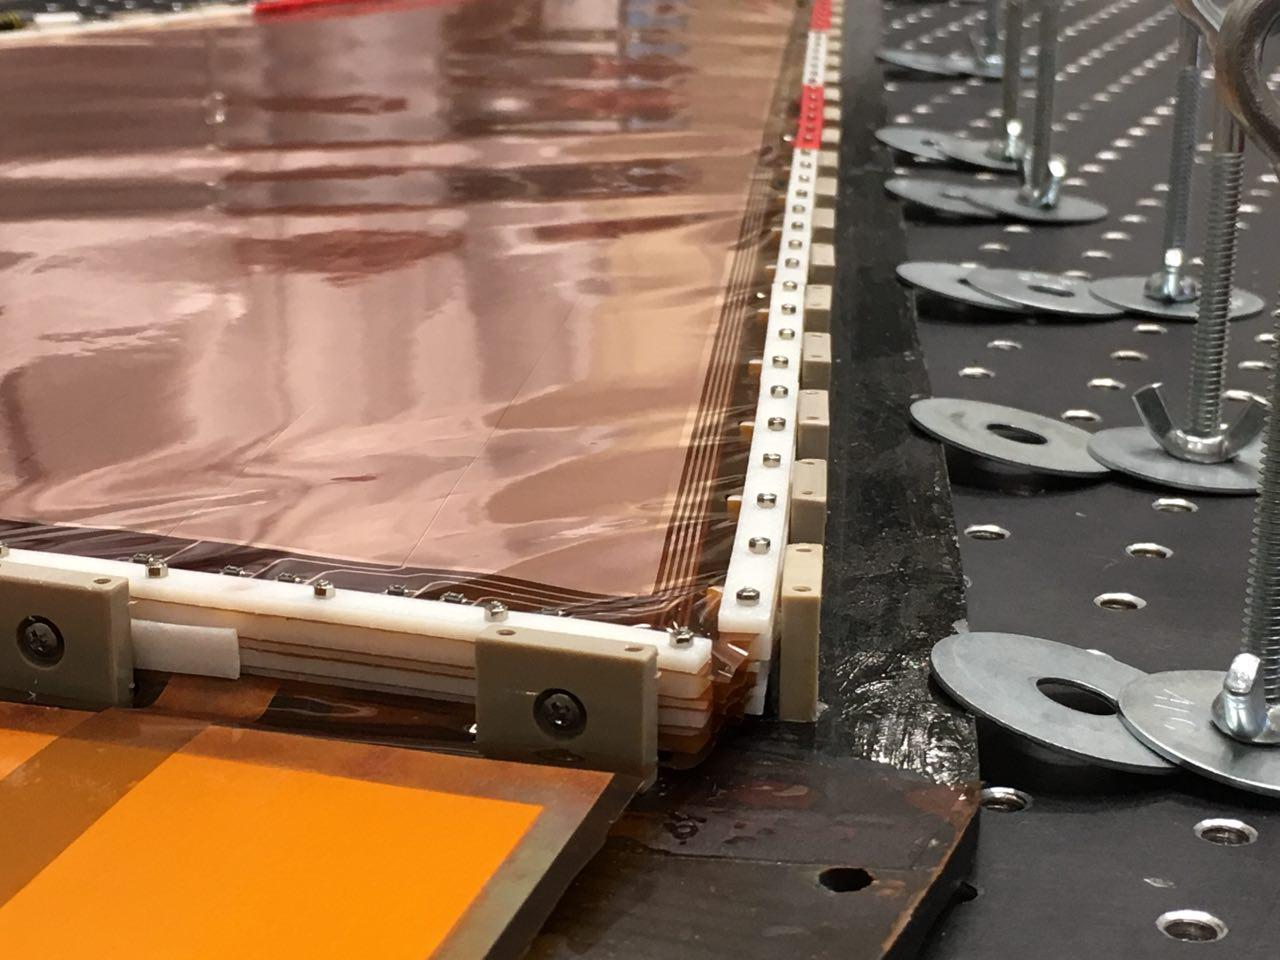
\includegraphics[width=0.9\textwidth]{FIT_plots/PEEK_Installation.jpg} 
	\caption{Test installation of PEEK pull-outs (gray blocks) in the low-mass GEM prototype.}
	\label{fig:installation}
\end{figure}

However, just as before we still observe shorts in the original GEM stack between those foils that are only 1 mm apart. To increase the spacing in the GEM stack, two new PEEK layers of inner frames with 2 mm thickness are being implemented. This will result in a stack with 3-2-2-2 mm gaps (drift, transfer 1, transfer 2, induction) instead of the previous 3-1-2-1 mm spacing. This replacement is possible due to the purely mechanical construction and stretching technique that we employ for the prototype.

For producing the pull-out parts, a 12"$\times$12" plate of 6 mm thick PEEK was machined on campus. In the original design of the inner frames, all pieces had the same short length of about 10 cm with 1 cm gaps between them. This resulted in warping of the GEM foils in the gaps. In the new design (Fig.\ref{fig:sidemid}), the side frames will be longer and fewer - more similar to the frame design of the CMS GE1/1 GEMs that this prototype is based on. The proper power setting of a laser cutter is currently being inverstigated for machining the inner frame pieces from a 12"$\times$6" plate of 2 mm thick PEEK, which is too thin for cutting on a NC machine. 

\begin{figure}[h]
	\centering
	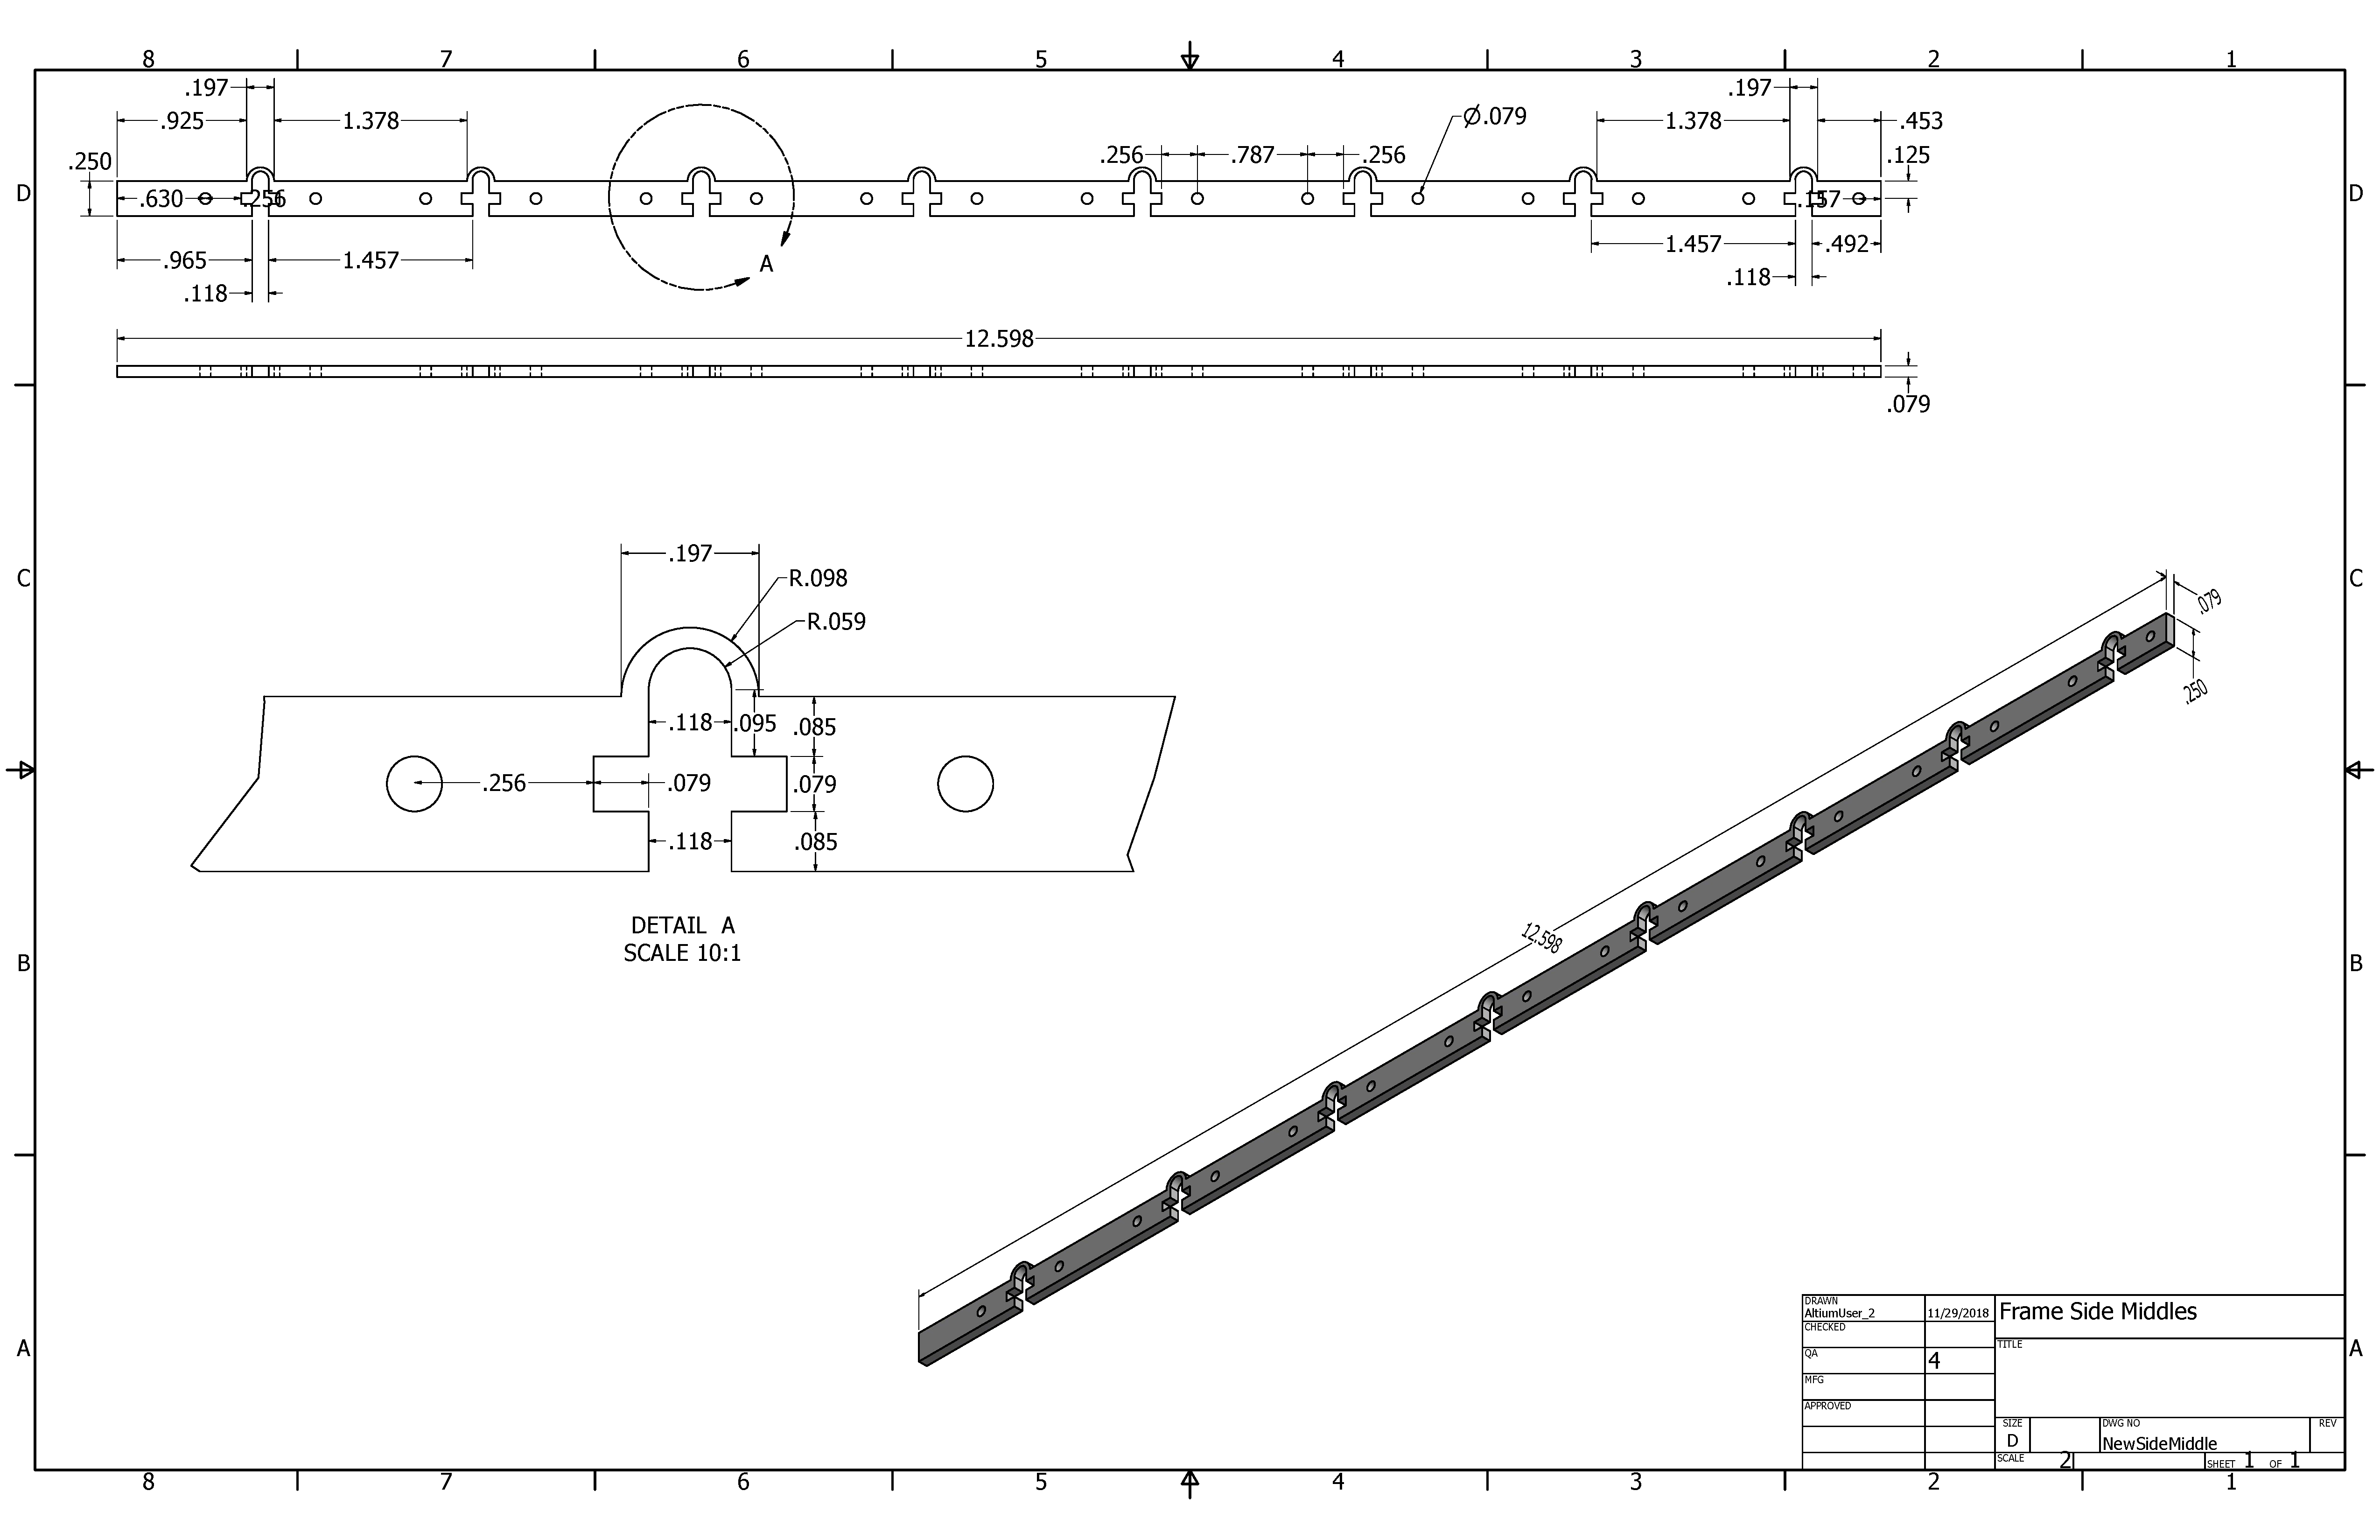
\includegraphics[width=0.9\textwidth]{FIT_plots/NewSideMiddle.pdf} 
	\caption{Design of longer middle sections of 2 mm side frames using PEEK.}
	\label{fig:sidemid}
\end{figure}



\paragraph*{R\&D on $\boldmath{\mu}$RWELL detector:} We have ordered a 10$\times$10 cm$^2$ resistive micro-well detector from CERN to begin some basic R\&D on this detector technology for fast tracking in the barrel region of the EIC detector. To complement the 2D readout with Cartesian strips chosen by the UVa group for their $\mu$RWELL detector prototype, we opted for a 1D zigzag strip readout foil based on the foil design that we had used for the 10$\times$10 cm$^2$ prototype\cite{Zhang:2017dqw} of the low-mass FT detector. We expect to receive this small detector in August or September 2018.



\paragraph*{EIC Simulations:} Undergraduate student Matt Bomberger continued his work on EIC simulations for investigating the impact that material budgets in the forward and backward regions will have on the overall EIC detector performance. He went to BNL in early August for a week to work directly with EicRoot expert Alexander Kiselev on the implementation of a forward tracker simulation based on Triple-GEMs. Working with a second undergraduate back at FIT, he succeeded in installing EicRoot in a Docker environment as well as directly in a CENTOS7 environment.

For a first study, he compared the momentum resolution of tracks measured with GEM chambers with standard copper foils vs.\ those with two chromium foils. A 3-1-2-1 mm GEM gap configuration and a beam of 1 GeV/c electrons emitted from the IP at 25$^\circ$ to the beamline are used. The geometry of this study and an example track are shown in Figure \ref{fig:geom}.

\begin{figure}[h]
	\centering
	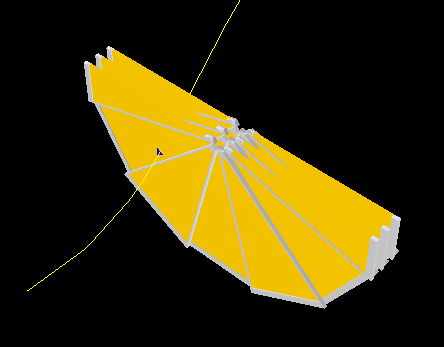
\includegraphics[width=0.9\textwidth]{FIT_plots/Geom_CrStdComp} % 
	\caption{EICroot simulation of a 1 GeV/c electron track reconstructed with 3 GEM rings in forward tracker region.}
	\label{fig:geom}
\end{figure}

The first configuration comprises all standard GEM foils, i.e.\ 5 $\mu$m thick planes of copper on both sides of a 50 $\mu$m thick plane of polyimide material. The distribution of the differences between reconstructed momentum and MC-truth momentum for this configuration has a Gaussian shape with a root mean square of 8.5\% (Figure \ref{fig:resolutions}(left)). For the configuration with chromium GEM foils, a 50 $\mu$ thick plane of polymide should be sandwiched between two planes of 200 nm thick planes of chromium. Since no direct method of using chromium foils is possible in EicRoot, the thickness of copper that would be equivalent to 2 foils with 200 nm of chromium and one of 5 $\mu$m of copper is plugged into the variable defining the thickness of copper in the GEM foils. In effect, this reduces the amount of copper basically by a factor three. The Gaussian plot of events versus momentum resolution for this chromium GEM configuration has an associated root mean square of 8.3\%. Comparing the RMS values for standard and chromium GEMs, one can see that they differ by only 0.2\% in favor of the chromium configuration. This implies that reducing the material from copper to chromium in two of the GEM foils has a minimal impact on the momentum resolution for this scenario. 

\begin{figure}[h]
	\centering
	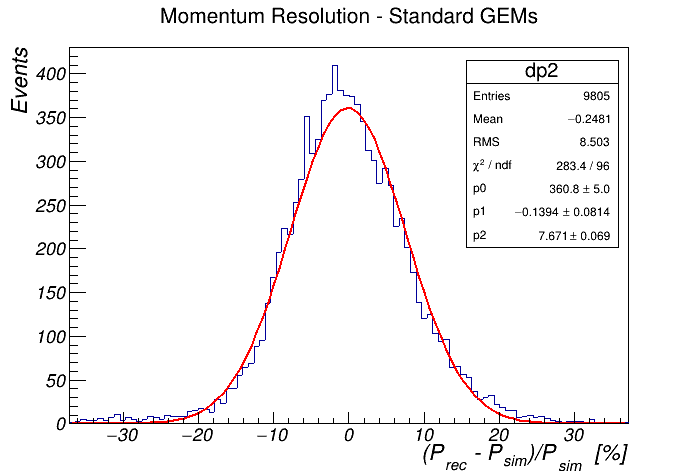
\includegraphics[width=0.49\textwidth]{FIT_plots/MomResStdGEM_25deg1GeV_101818}
	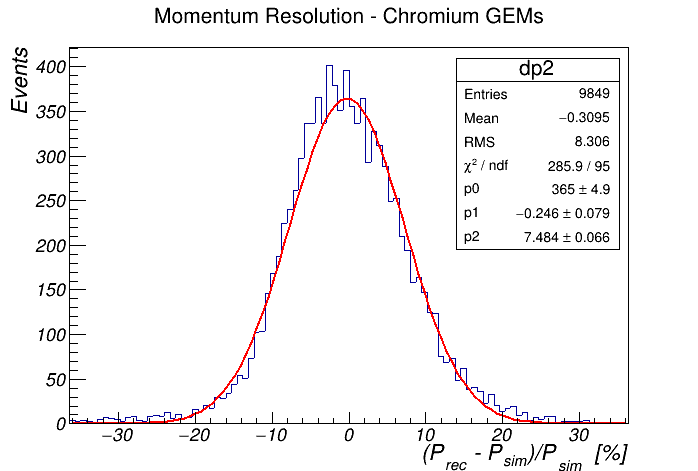
\includegraphics[width=0.49\textwidth]{FIT_plots/MomResCrGEM_25deg1GeV_101818} 
	\caption{Momentum resolutions for 1 GeV/c electron tracks measured with three rings of forward tracker GEMs in EICroot simulation (preliminary). Left: Standard GEMs with copper foils. Right: GEMs with two chromium foils and one copper foil.}
	\label{fig:resolutions}
\end{figure}




\subsubsection{INFN Trieste} 
\label{sec:INFN-achieved}
\textbf{Activity in period 
July 2018 - December 2018}
\par
\begin{enumerate}
\item
\textbf{Test beam studies of a prototype of the single photon detector 
by MPGD technologies with miniaturized 
pad-size}\\
The prototype architecture consists in two 
staggered THGEM layers, the first one also acting 
as photocathode substrate, followed by a resistive MM 
by discrete elements. The detector active surface is 
100$\times$100~mm$^2$. The THGEM geometrical parameters 
are: 400~$\mu$m hole diameter, 800~$\mu$m pitch, 
400~$\mu$m thickness and hole without a rim.
The MM has 128~$\mu$m gap; the 
pad-size is 3$\times$3~mm$^2$ with 
3.5~mm pitch, forming a matrix  of 
32$\times$32 pads (in total 1024 pads). 
The pads are 
grouped in 32$\times$4  modular 
units; each unit is equipped with a 
connector interfacing the signal 
pads to the front-end electronics 
and a second, identical connector, 
providing the biasing voltage to the 
anode pads via protection resistors, 
one per pad, housed in a dedicated 
resistor board. Figure~\ref{fig:espanso-ibrida}
illustrates the detector design.
The prototype has been built
and fully tested in laboratory, as reported 
in July 2019. The main exercise of the present
reporting period concerns the test beam studies of
the prototype performed at CERN over  two weeks
between the end of October and the beginning
of November 2018. During the test-beam period, we have been main-users for part of the time and otherwise we have worked in parasitic mode. High energy ($>$100~GeV) muons or pions have been alternatively delivered.
%%%%%%%%%%%%%%%%%%%%%%%%%%%%%
\begin{figure}
			\begin{center}
		   		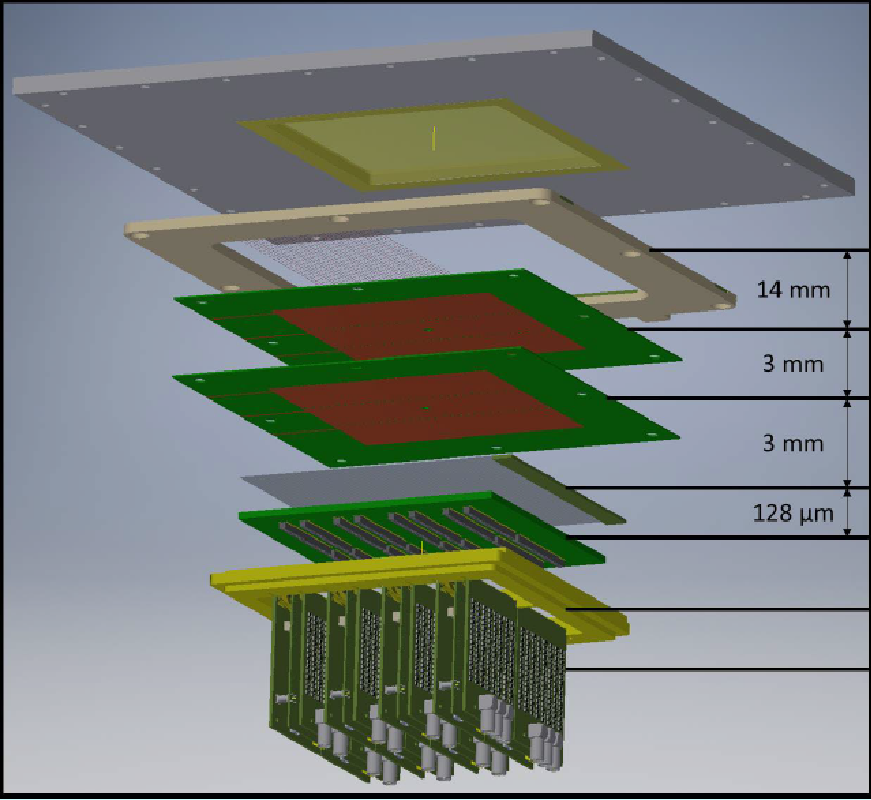
\includegraphics[width=0.7\textwidth]{INFN_plots/espanso-ibrida}
				\caption{\label{fig:espanso-ibrida}
                Exploded view drawing of the prototype.}
          		\end{center}
			\end{figure}
          \par     A compact test-beam setup was
	prepared, assembled and equipped in Trieste
(Fig.~\ref{fig:set-up_sketch}). It includes:
\begin{itemize}
\item The mechanical support of the detectors; it houses also the HV and LV
	power supplies.
    \item The system of scintillation counters that
    form the trigger: four finger-shaped counters
    are used in coincidence, two placed upstream of
    the prototype and two downstream of it; in both
    couples, the detectors are arrange with
    orthogonal orientation, so to define a cross
    with a small overlap surface of
    3$\times$3~mm$^2$ for the first couple and
    5$\times$5~mm$^2$ for the second one. The
    purpose of this arrangement is to 
    select beam particles crossing the detector
    almost perpendicularly at a well-defined
    location; the position of the finger-shaped counters is
    remotely controlled by step motors to facilitate
    the alignment.
\item The prototype detector with its read-out electronics.
\item A fused silica radiator is mounted onto
    the prototype; it has cylindrical symmetry
    and a dedicated design: the majority of the Cherenkov photons
    generated by minimum ionizing particles with trajectories quasi-parallel to its axis hit the detector surface in a ring-shaped area
    (Figs.~\ref{fig:radiator}, \ref{fig:hybrid&radiator}). A shutter is situated between the radiator and the photocathode and it is remotely controlled via a piezoelectric actuator.
  
\item The read-out system is based on the SRS/APV25 system~\cite{1748-0221-8-03-C03015} developed within the RD51 collaboration. The 1024 pads are read-out by eight APV25 chips, 128 channel each. The chip control and the DAQ is ensured by the novel DAQ Raven system,  entirely
LabView based, developed within our R\&D activity in order  to ensure large acquisition band width. The Raven  system architecture and performance have been reported about in January 2018. Dedicated interface boards have been designed and realized to interface the detector connectors and the SRS/APV25 FE boards.
\end{itemize}
%%%%%%%%%%%%%%%%%%%%%%%%%%%%%%%
\begin{figure}
\begin{center}
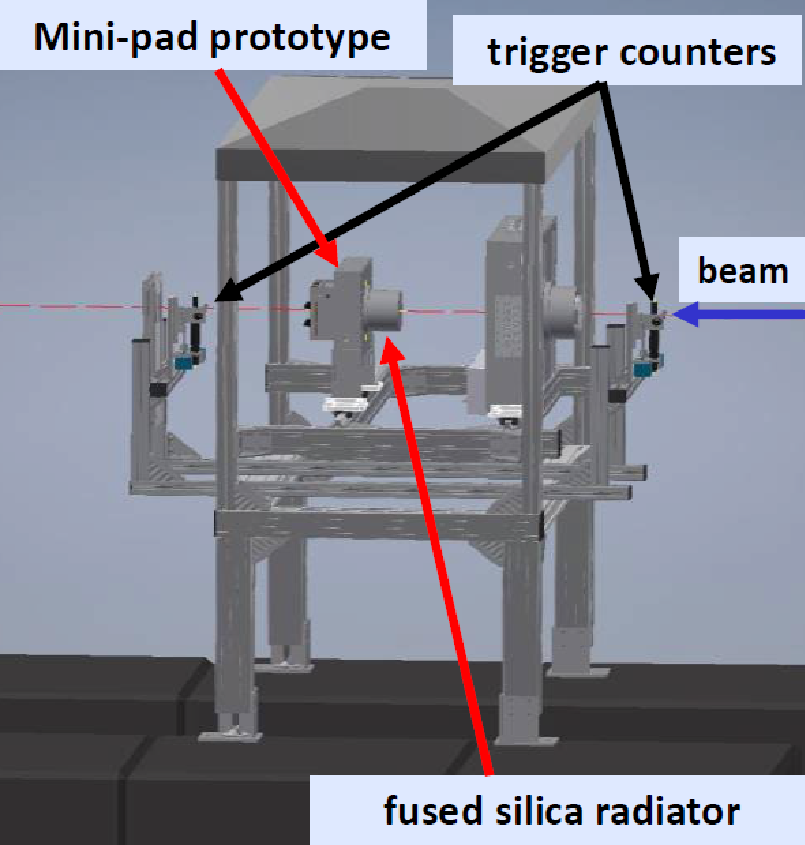
\includegraphics[width=0.6\textwidth]{INFN_plots/set-up_sketch}
\caption{\label{fig:set-up_sketch}
Sketch of the test-beam set-up.
}
\end{center}
\end{figure}
%%%%%%%%%%%%%%%%%%%%%%%%%%%%%%%%%%%%%%%%%%%%%%%%%%%%%%%%%
\begin{figure}
			\begin{center}
            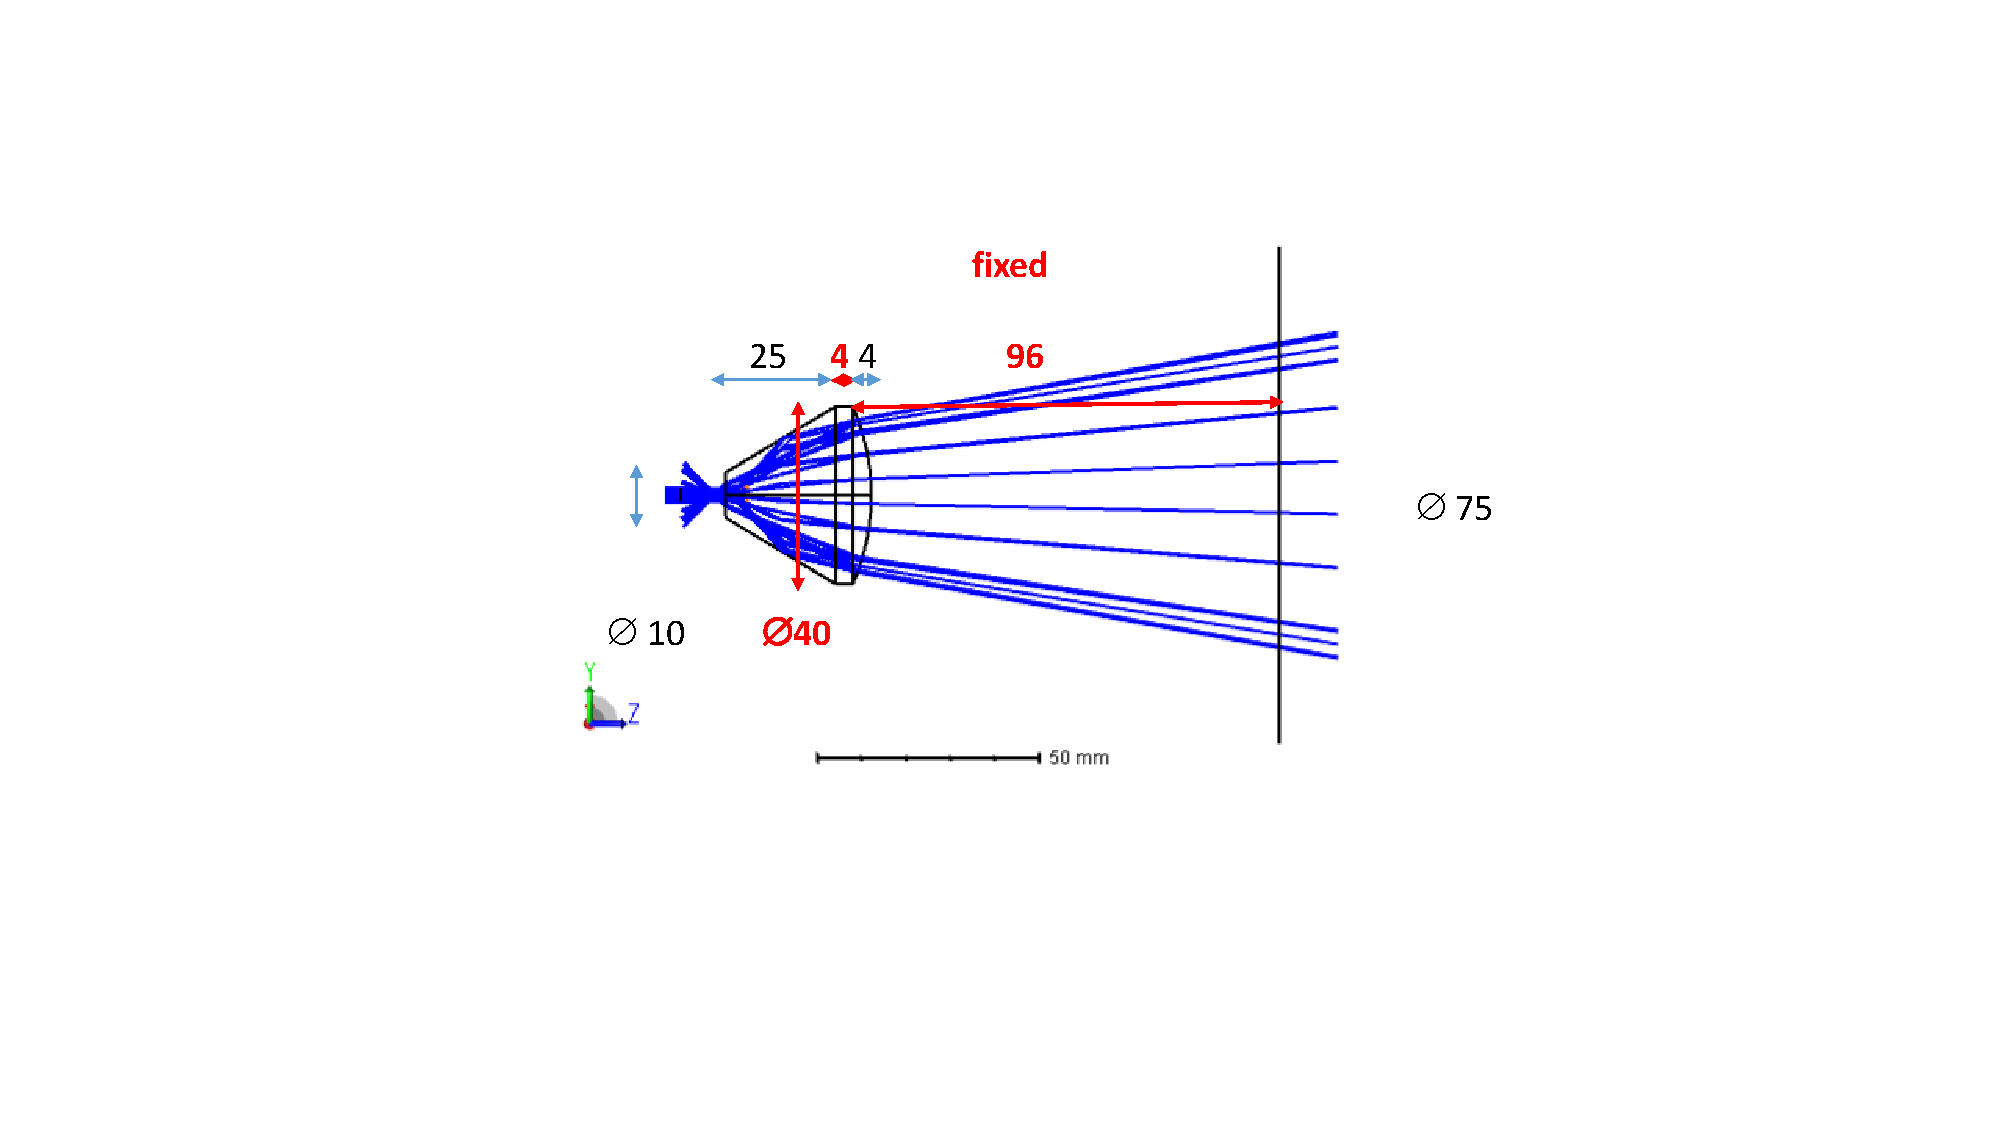
\includegraphics[width=0.7\textwidth]{INFN_plots/radiator}
\caption{\label{fig:radiator}
Cross-section of the fused silica radiator with cylindrical symmetry. The blue lines are examples of Cherenkov photon trajectories; a large fraction of them intercepts the photocathode surface (the vertical black line in the drawing) in a ring-shaped region, even if some of the photons hit the photocathode in different areas. The majority of the photons generated in the radiator are trapped inside the radiator itself due to total reflection; there are no examples of these trajectories in the drawing.
}
			\end{center}
\end{figure}
%%%%%%%%%%%%%%%%%%%%%%%%%%%%%%%
%%%%%%%%%%%%%%%%%%%%%%%%%%%
\begin{figure}
			\begin{center}
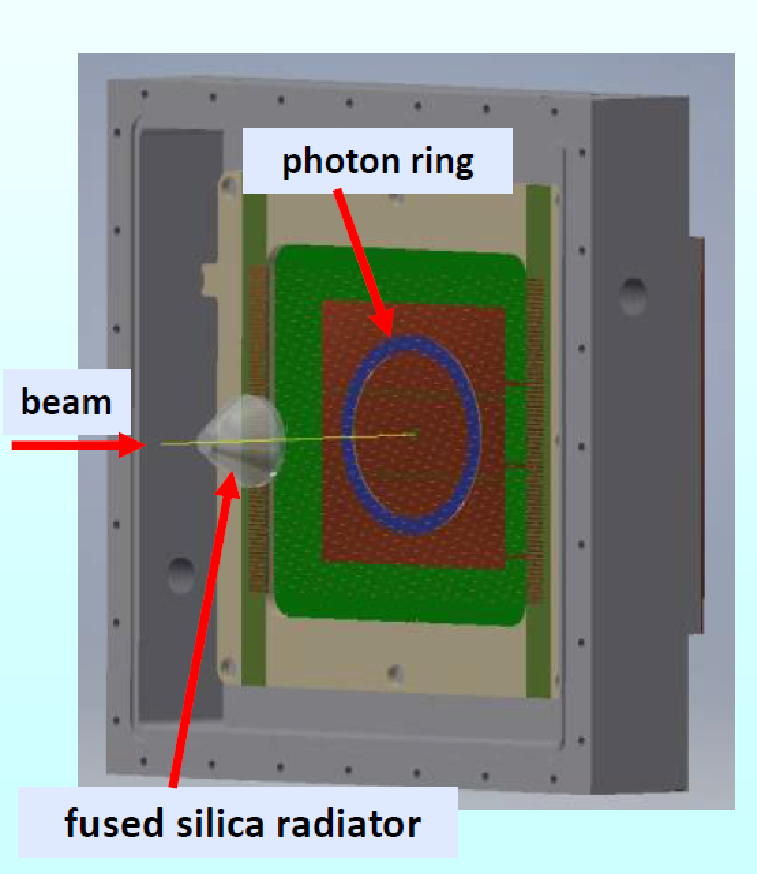
\includegraphics[width=0.6\textwidth]{INFN_plots/hybrid&radiator}
\caption{\label{fig:hybrid&radiator}
Skematic drawing illustrating the formation of the ring image in the photon detector by Cherenkov photons generated in the fused silica radiator. 
}
			\end{center}
\end{figure}
%%%%%%%%%%%%%%%%%%%%%%%%%%%%%%%
The last phase of the detector assembly consists in inserting in the detector the THGEM coated with the CsI film, that must not be expose to air in order to preserve its quantum efficiency. This implies that the final assembly is performed in a glove-box (Fig.~\ref{fig:assembly-in_glovebox}), including mounting  the fused silica radiator and the shutter. A picture of the prototype fully equipped and installed at the test-beam is shown in Fig.~\ref{fig:mini-pad_at_test-beam}.                 %%%%%%%%%%%%%%%%%%%%%%%%%
\begin{figure}
			\begin{center}
			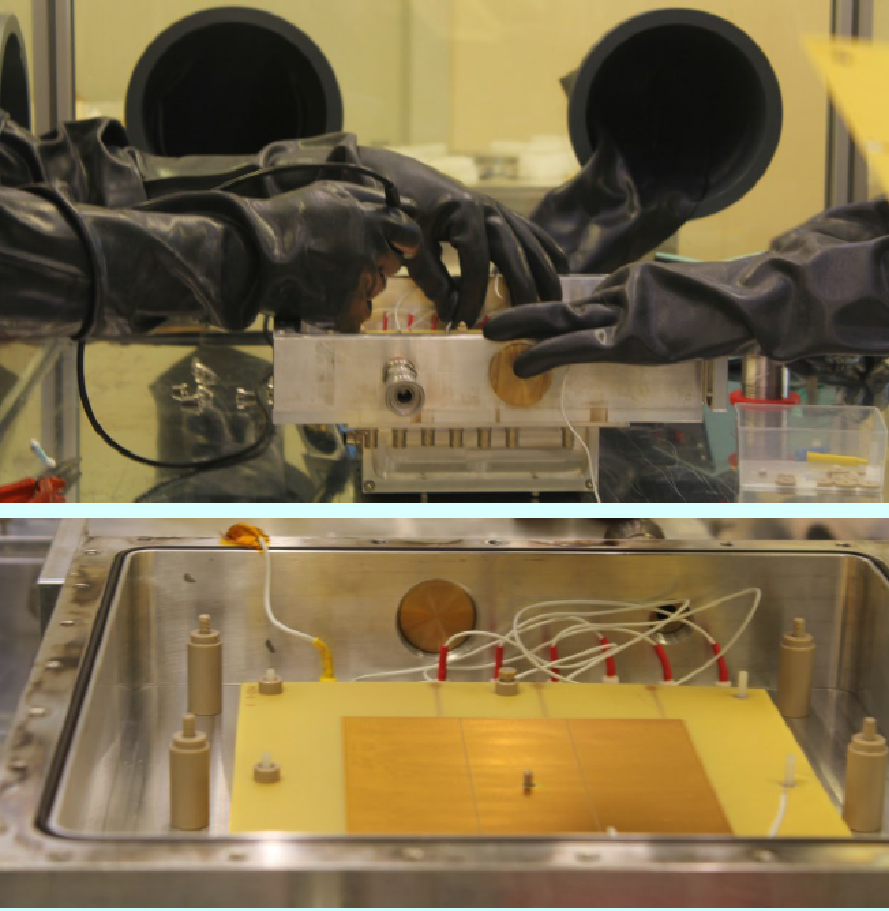
\includegraphics[width=0.6\textwidth]			
                {INFN_plots/assembly-in_glovebox}
				\caption{\label{fig:assembly-in_glovebox}
                	Pictures illustrating the final phase of the 
       						 prototype
               	assembly, which is performed in a glove-box.
               	 }
			\end{center}
            \end{figure}%%%%%%%%%%%%%%%%%%%%%%%%
\begin{figure}
			\begin{center}
			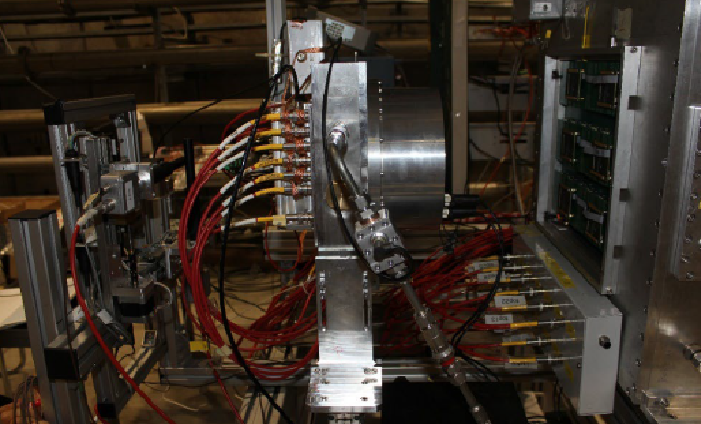
\includegraphics[width=0.6\textwidth]
                			{INFN_plots/mini-pad_at_test-beam}
				\caption{\label{fig:mini-pad_at_test-beam}
                Picture of the fully-equipped prototype 
                		installed at the
                test-beam.
                }
			\end{center}
            \end{figure} 
            %%%%%%%%%%%%%%%%%%  
       Data have been collected using two different gas mixture, 
       namely (a) Ar:CH$_4$~=~50:50 and (b) pure methane, and different voltage settings in order 
       to determine the 
       optimal operation conditions. The data analysis has just 
       started and in the following we provide some preliminary 
       information obtained from the data collected with gas 
       mixture (a) and with the muon beam. It is relevant to underline that, aiming at single 
       photoelectron detection, we have to deal with an exponential 
       amplitude spectrum, where the majority of the population is 
       at small amplitudes. Therefore, we have to apply to the signals small 
       threshold-values and a good control of the noise 
       is important. At present, in the data analysis, we have not yet implemented the 
       subtraction of the common-mode noise and, therefore, the 
       following preliminary plots are still affected by 
       non-negligible noise contributions. In this preliminary analysis, the software threshold applied to the amplitude is at the level of 4.5$\times$ the noise r.m.s. . For each event and for each read-out channel, 27 consecutive amplitude measurements are registered. The time distance between two consecutive measurements is 25~ns.
       The time development of a typical signal is shown in Fig.~\ref{fig:APV_signal}:  the 27 consecutive measurements of the signal amplitude  in all the 128 channels of an APV25 chip are shown. A signal is present in one of the channels. The plot has ben obtained on-line using one of the features of the Raven DAQ system.  In the following, the time respect to the trigger associated to the heighest amplitude of a channel is used: the resulting time distribution of the signals with amplitude above threshold is shown in Fig.~\ref{fig:timing_plot-1}.  A clean peak is visible fully contained in bins: 6-10, namely in a 125~ns time interval; in the following a corresponding time-cut is applied. \par    %%%%%%%%%%%%%%%%%%%%%%%%
\begin{figure}
			\begin{center}
			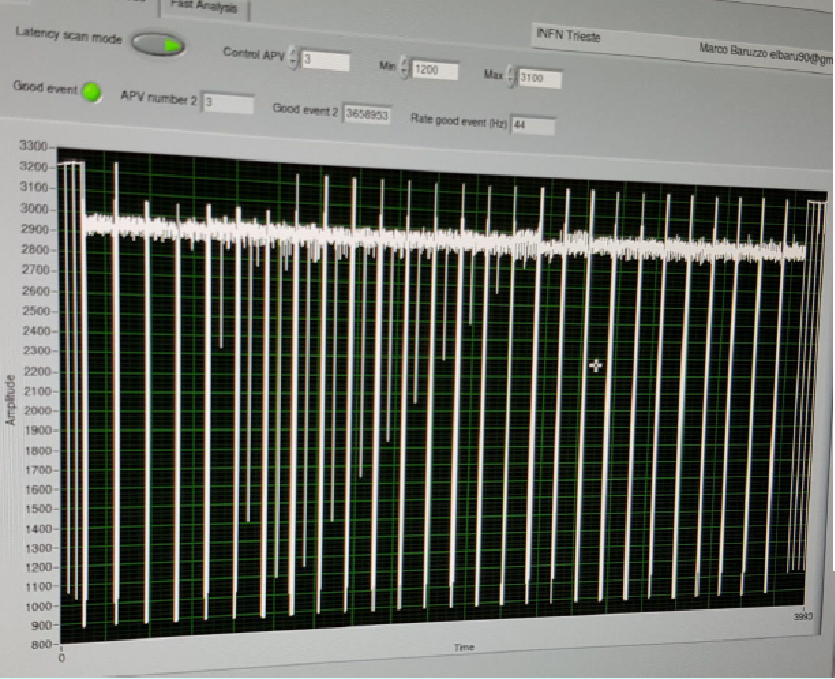
\includegraphics[width=0.6\textwidth]
                			{INFN_plots/APV_signal}
				\caption{\label{fig:APV_signal}
               27 consecutive measurements of the signal amplitude  in all the 128 channels of an APV25 chip are shown; the time interval between two consecutive measurements is 25~ns. The development of a physical signal versus time can be seen in one of the APV25 channels.
                }
			\end{center}
            \end{figure} 
            %%%%%%%%%%%%%%%%%%  %%%%%%%%%%%%%%%%%%%%%%%%
\begin{figure}
			\begin{center}
			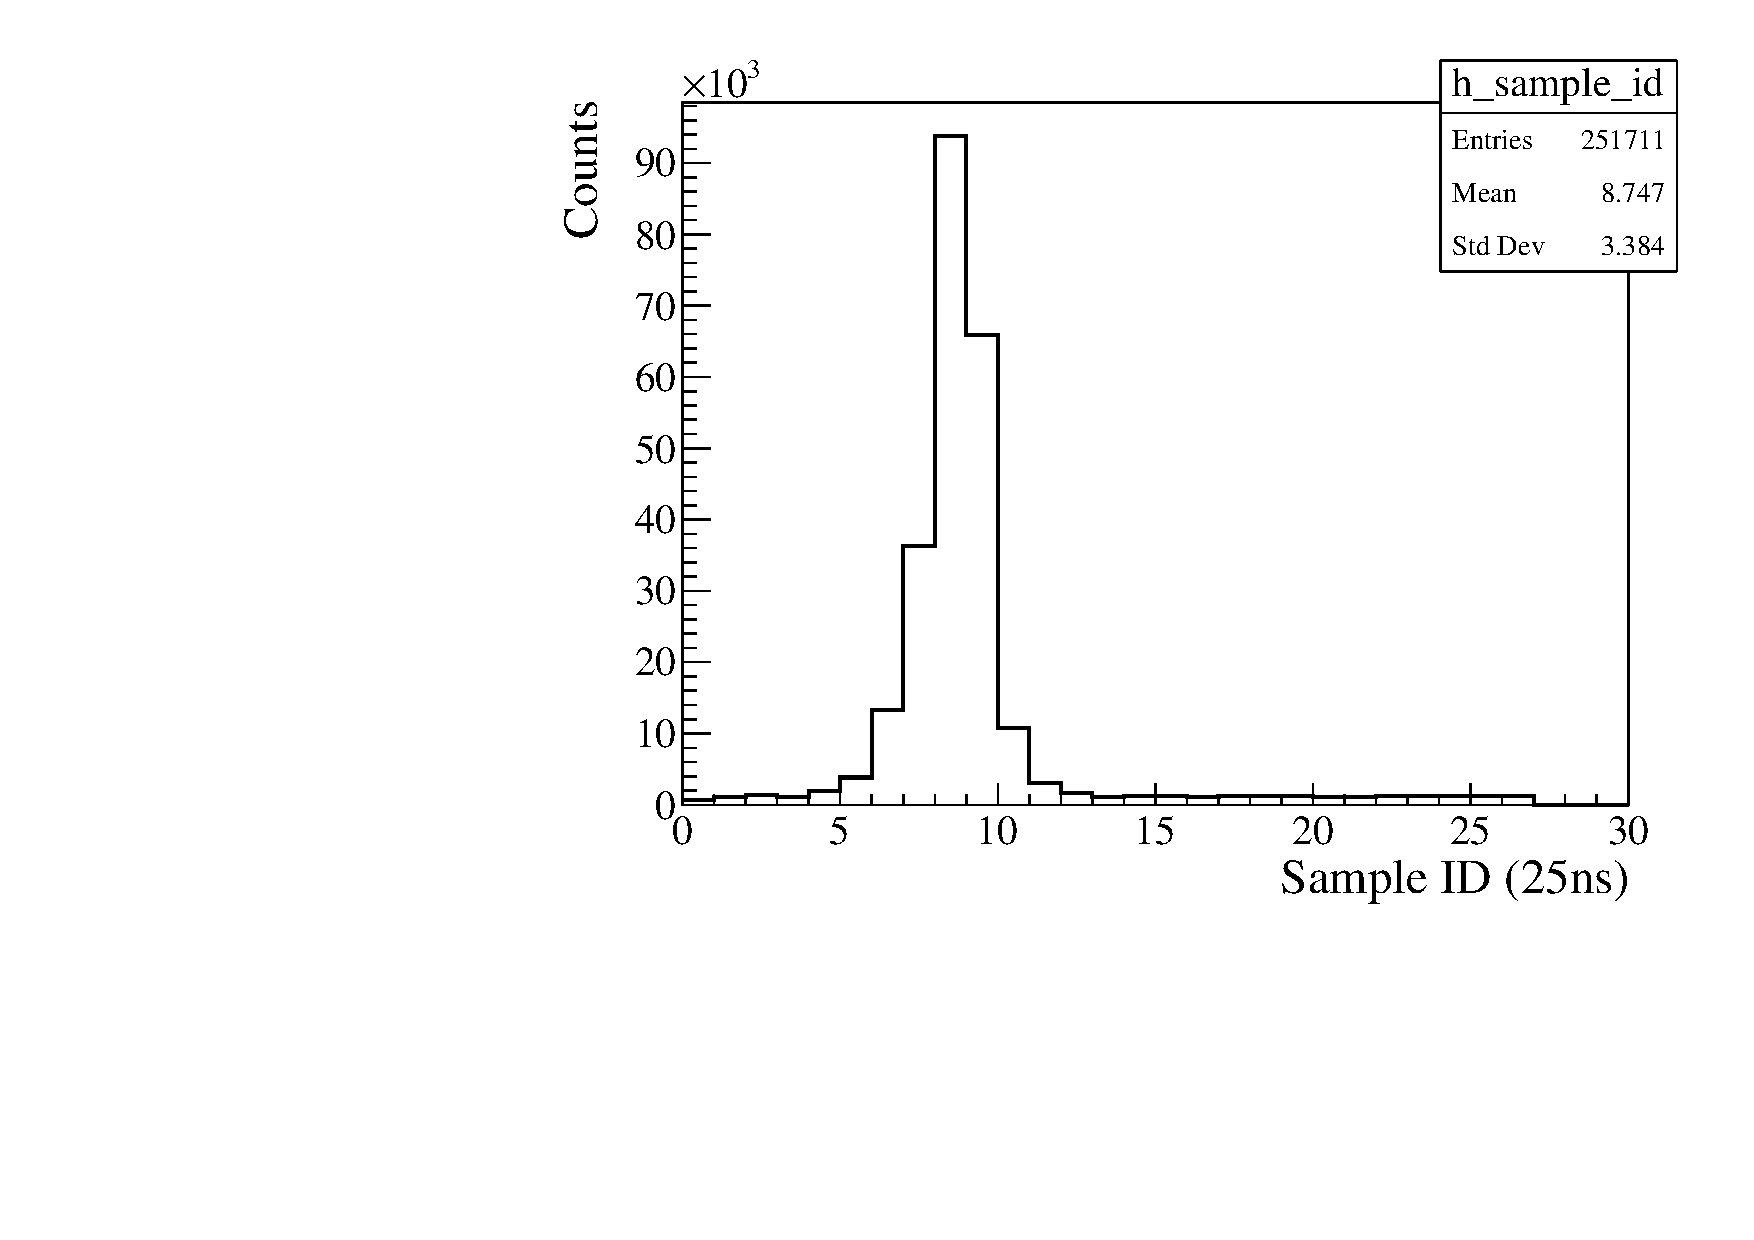
\includegraphics[width=0.6\textwidth]
                			{INFN_plots/timing_plot-1}
				\caption{\label{fig:timing_plot-1}
               Time distribution of the signals respect to the trigger 
               time. }
			\end{center}
            \end{figure} 
            %%%%%%%%%%%%%%%%%%  \par
       The 2-D histogram of the hits for a sample of events collected with the shutter between the radiator and the photocathode open is shown in Fig.~\ref{fig:Iris_open_Ar_CH4}. A ring is clearly visible as well as, at the center of the ring, the hits due to the minimum ionizing particles crossing the detector. In a corresponding histogram for data collected with the shutter closed (Fig.~\ref{fig:Iris_closed_Ar_CH4}) the ring is no longer visible, while the particle signal is still present. Subtracting the second histogram from the first one applying proper normalization with the ration of the number of events in the two samples, the particle signal disappears, while the ring is clearly visible and, outside the ring-region, the population in the histogram bins fluctuates around zero. (Fig.~\ref{fig:subtraction_open_close_Ar_CH4_2D-2}).  Therefore, it can be concluded that Cherenkov photons are clearly detected.   \par   %%%%%%%%%%%%
\begin{figure}
			\begin{center}
			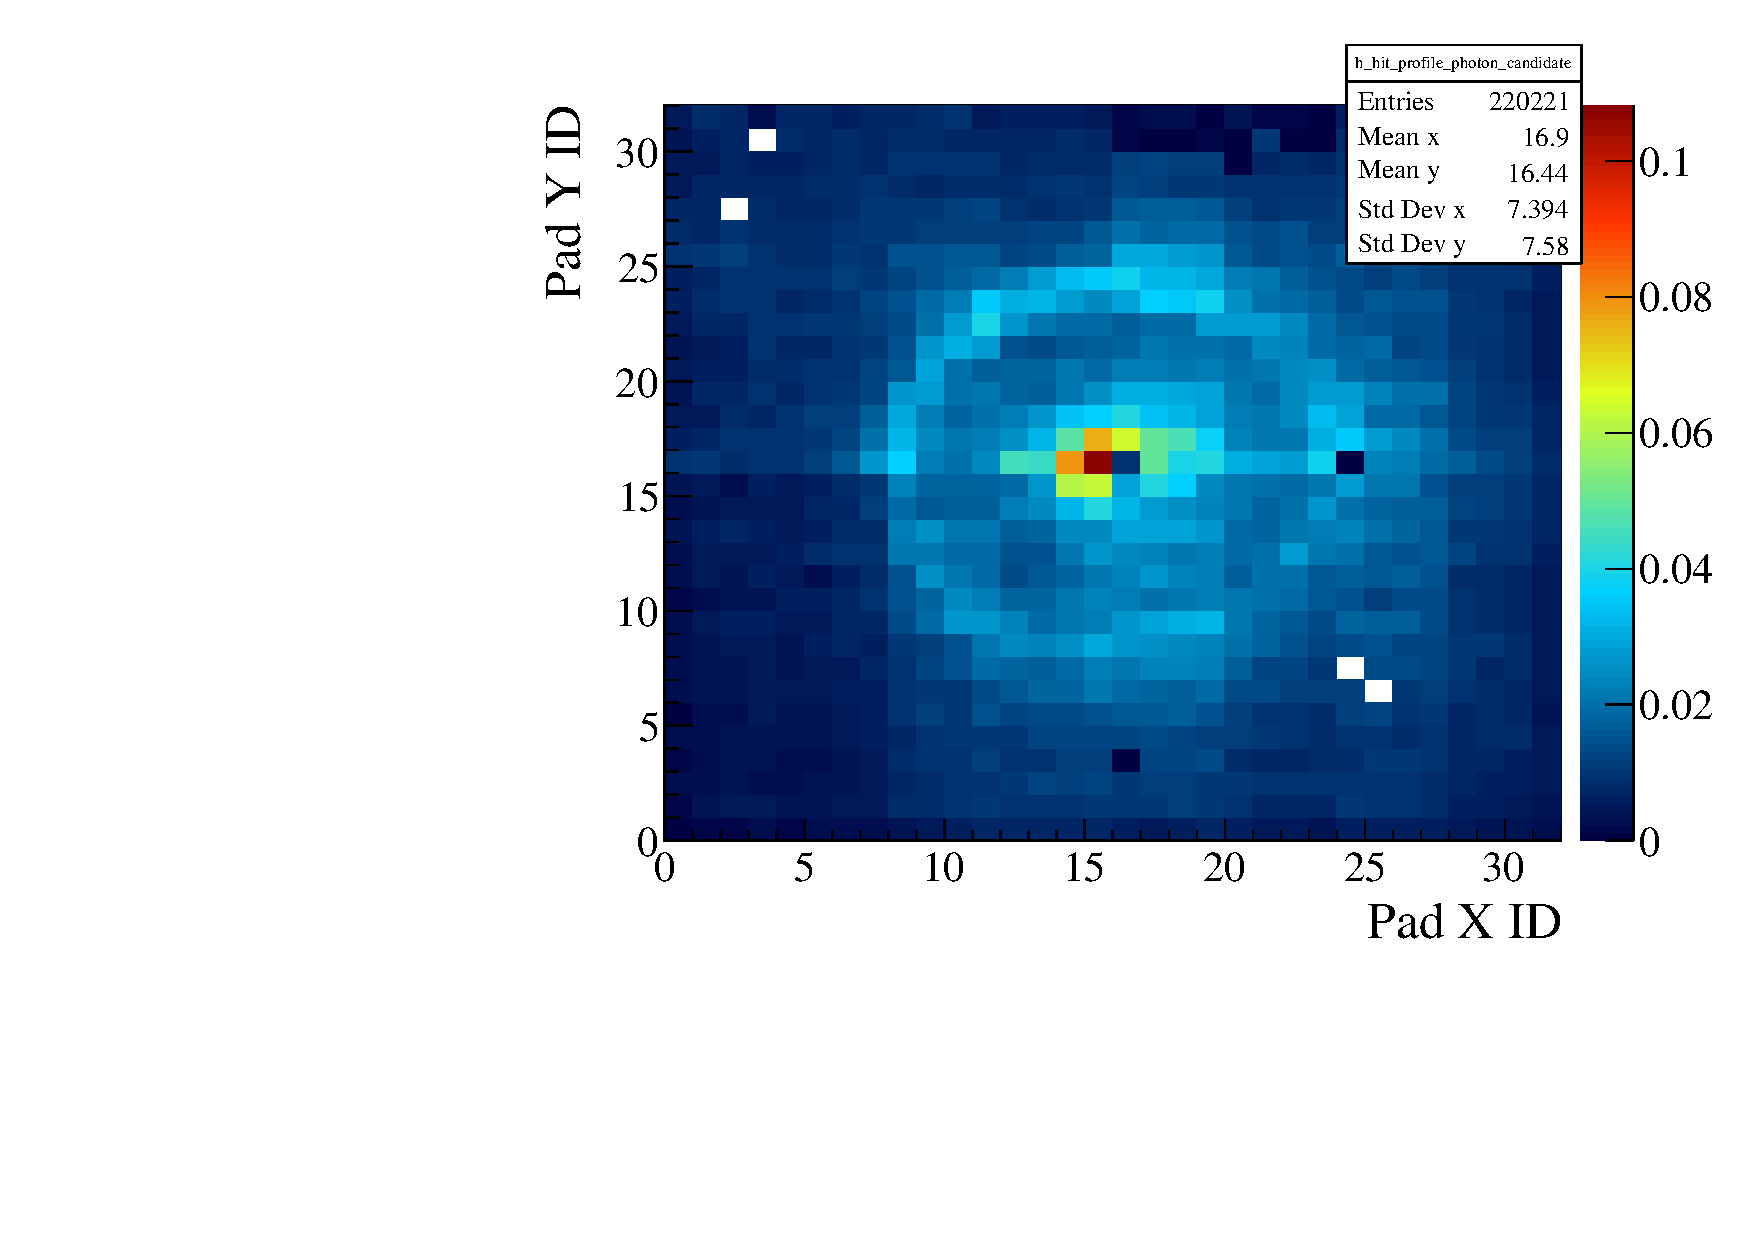
\includegraphics[width=0.6\textwidth]
                			{INFN_plots/Iris_open_Ar_CH4}
				\caption{\label{fig:Iris_open_Ar_CH4}
              2-D histogram of the hits for a sample of events collected with the shutter between the radiator and the photocathode open.}
			\end{center}
            \end{figure} 
            %%%%%%%%%%%%%%%%%%  %%%%%%%%%%%%
\begin{figure}
			\begin{center}
			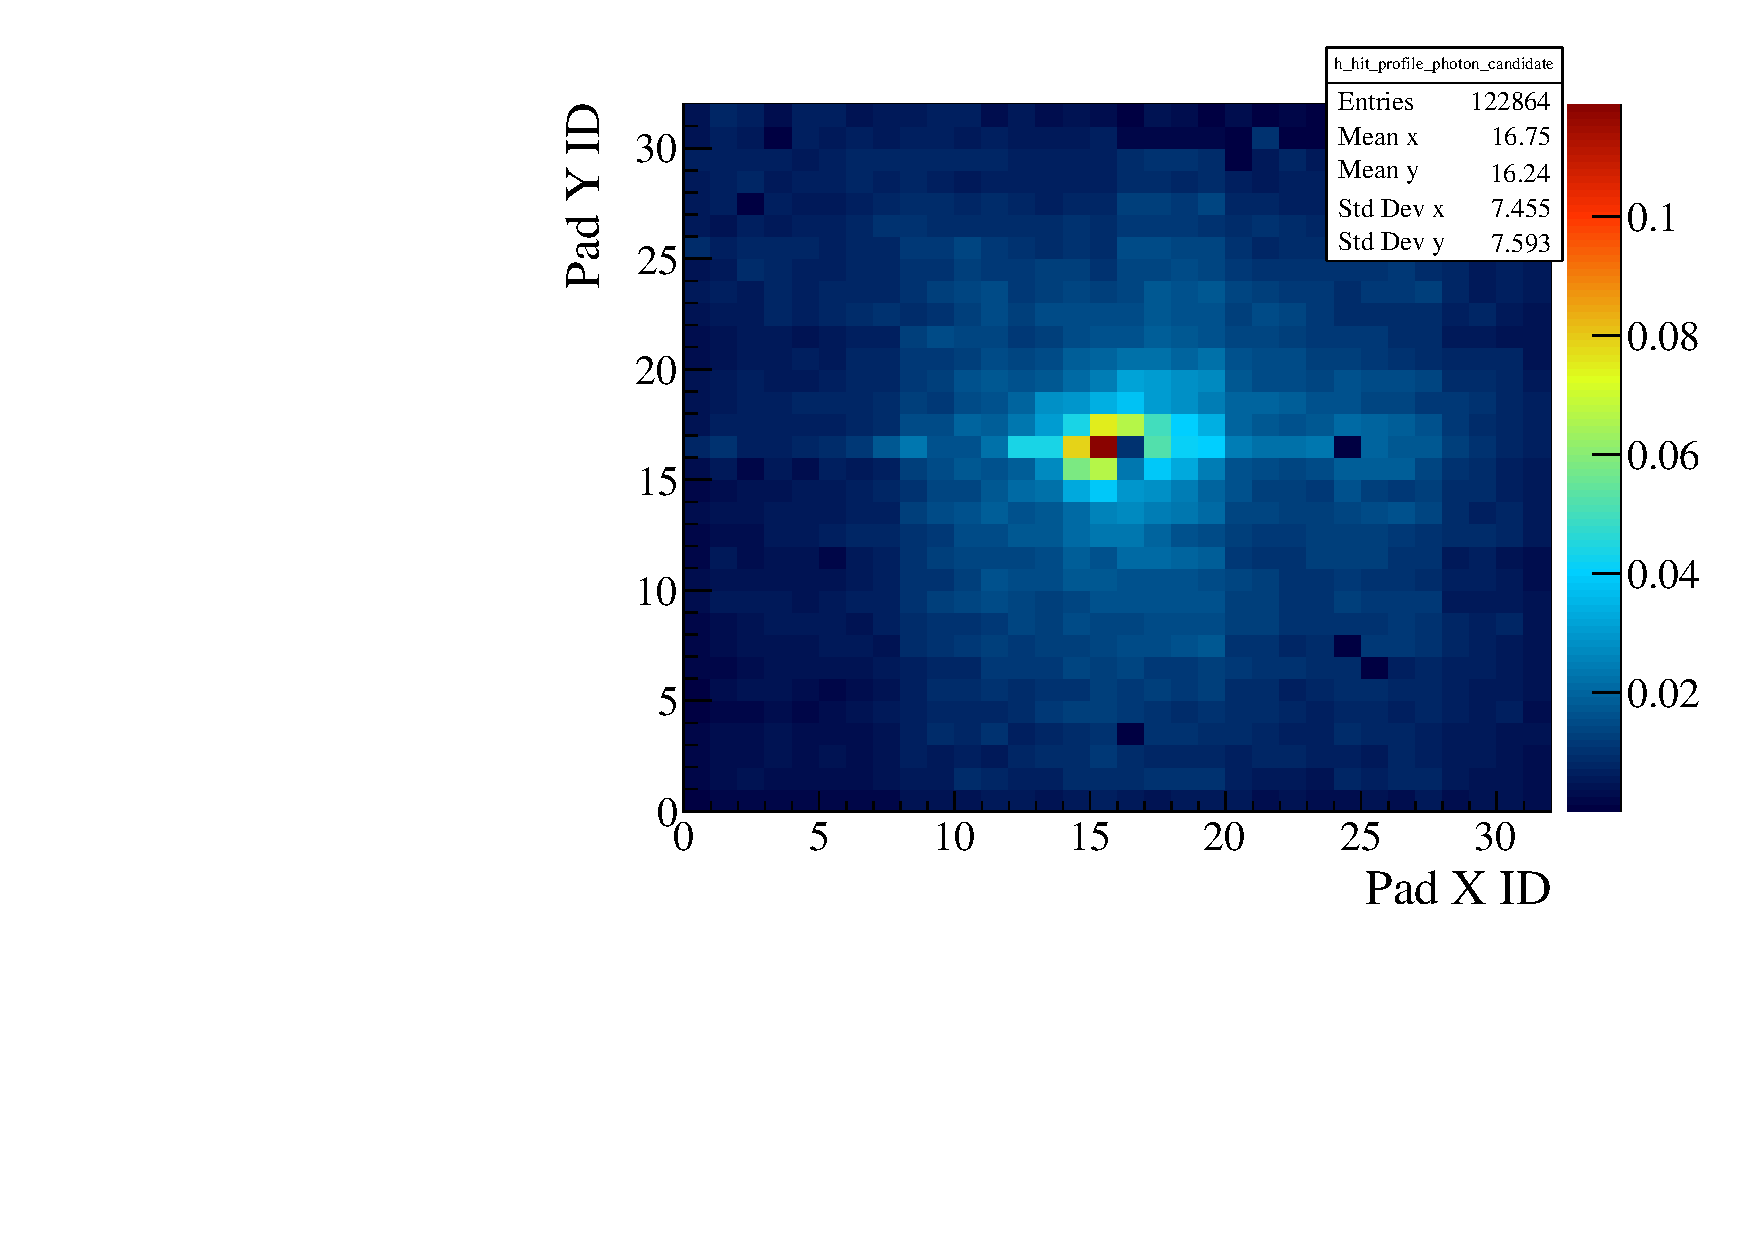
\includegraphics[width=0.6\textwidth]
                			{INFN_plots/Iris_closed_Ar_CH4}
				\caption{\label{fig:Iris_closed_Ar_CH4}
             2-D histogram of the hits for a sample of events collected with the shutter between the radiator and the photocathode closed.  }
			\end{center}
            \end{figure} 
            %%%%%%%%%%%%%%%%%%   %%%%%%%%%%%%
\begin{figure}
			\begin{center}
			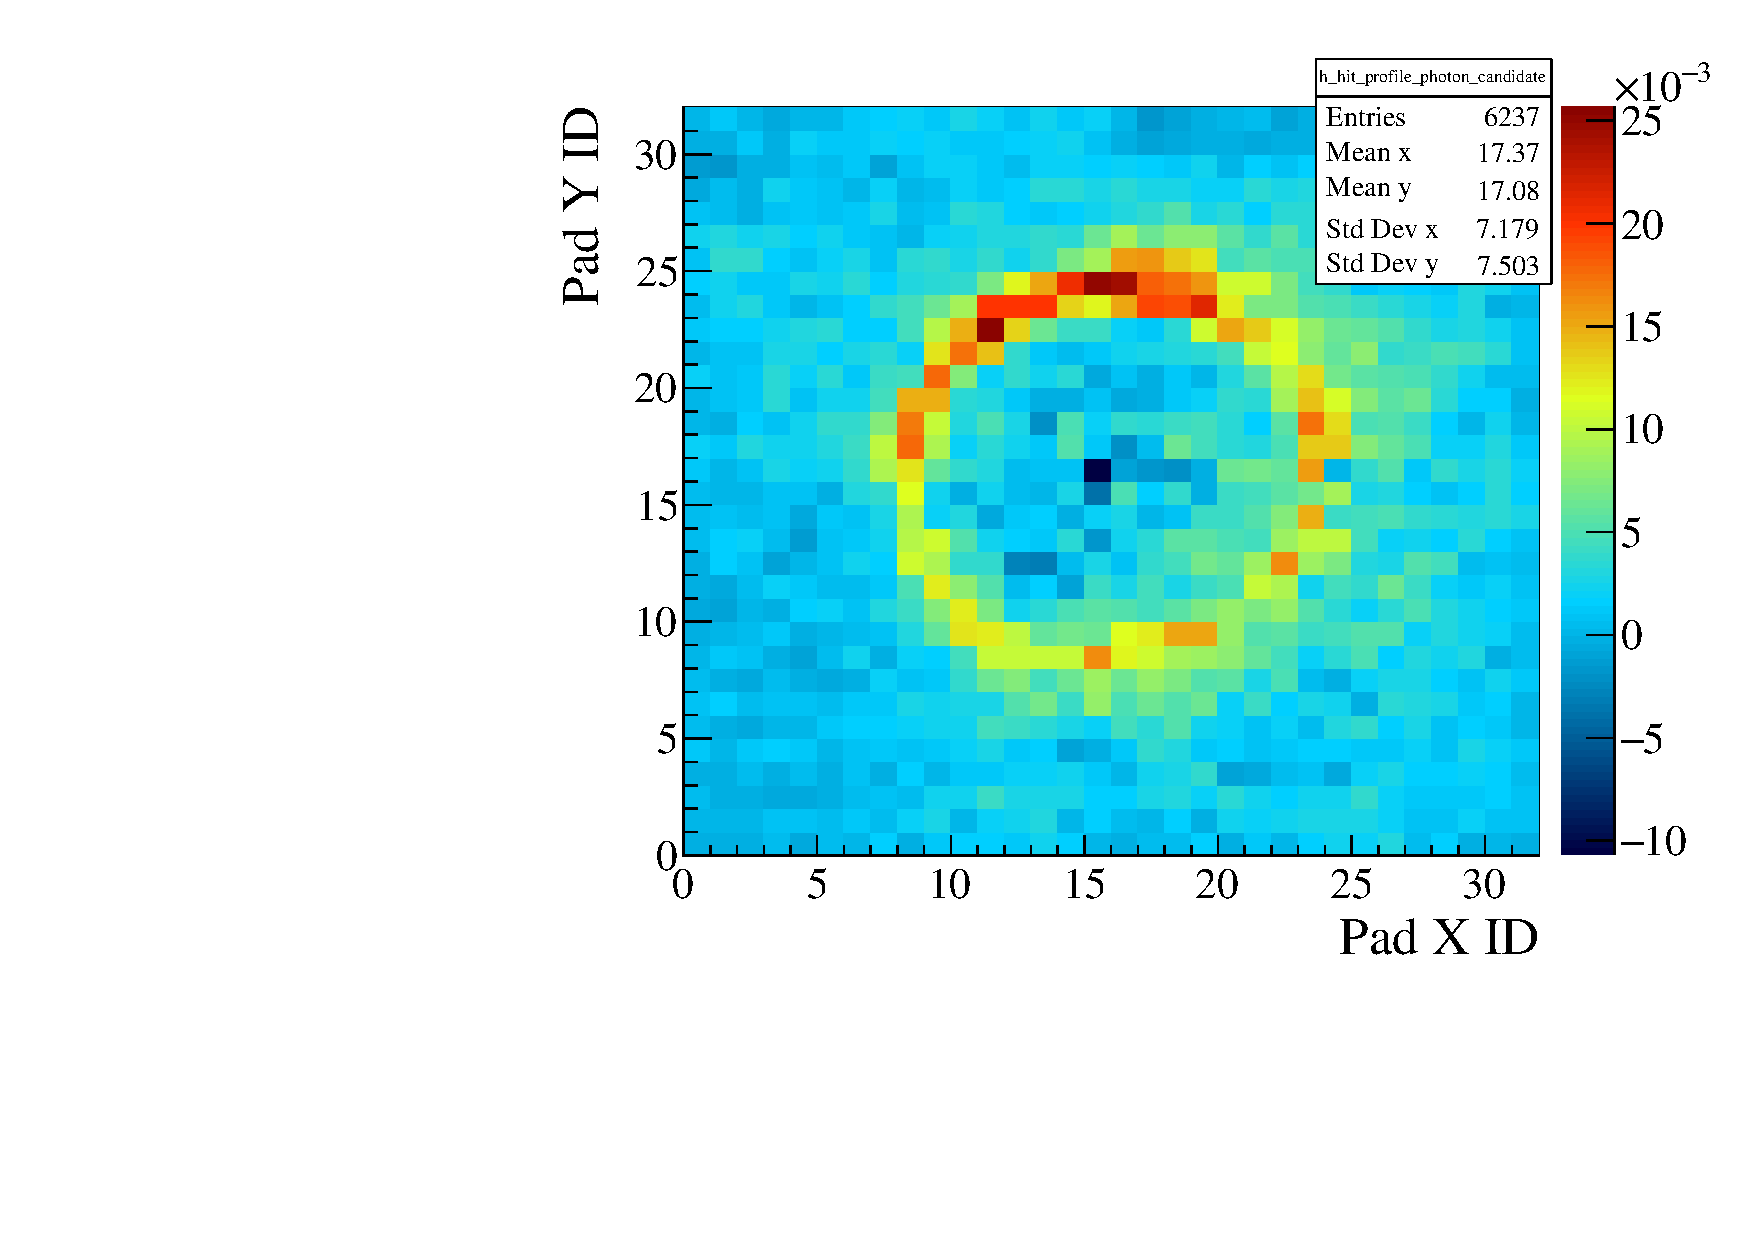
\includegraphics[width=0.6\textwidth]                	{INFN_plots/subtraction_open_close_Ar_CH4_2D-2}
				\caption{\label{fig:subtraction_open_close_Ar_CH4_2D-2}
              2-D histogram of the difference between the 2-D histograms for events collected with the shutter between the radiator and the photocathode open and closed. The histogram population has been normalized with the ratio of the number of events in the two samples. }
			\end{center}
            \end{figure} 
            %%%%%%%%%%%%%%%%%%\par
     A preliminary algorithm performing hit clusterization is applied to the hits in the ring area. The distribution of the cluster amplitude is used to extract information about the detector gain, as shown in Fig.~\ref{fig:cluster_gain_fit}: the resulting gain has the remarkable value of 50k. %%%%%%%%%%%%
\begin{figure}
			\begin{center}
			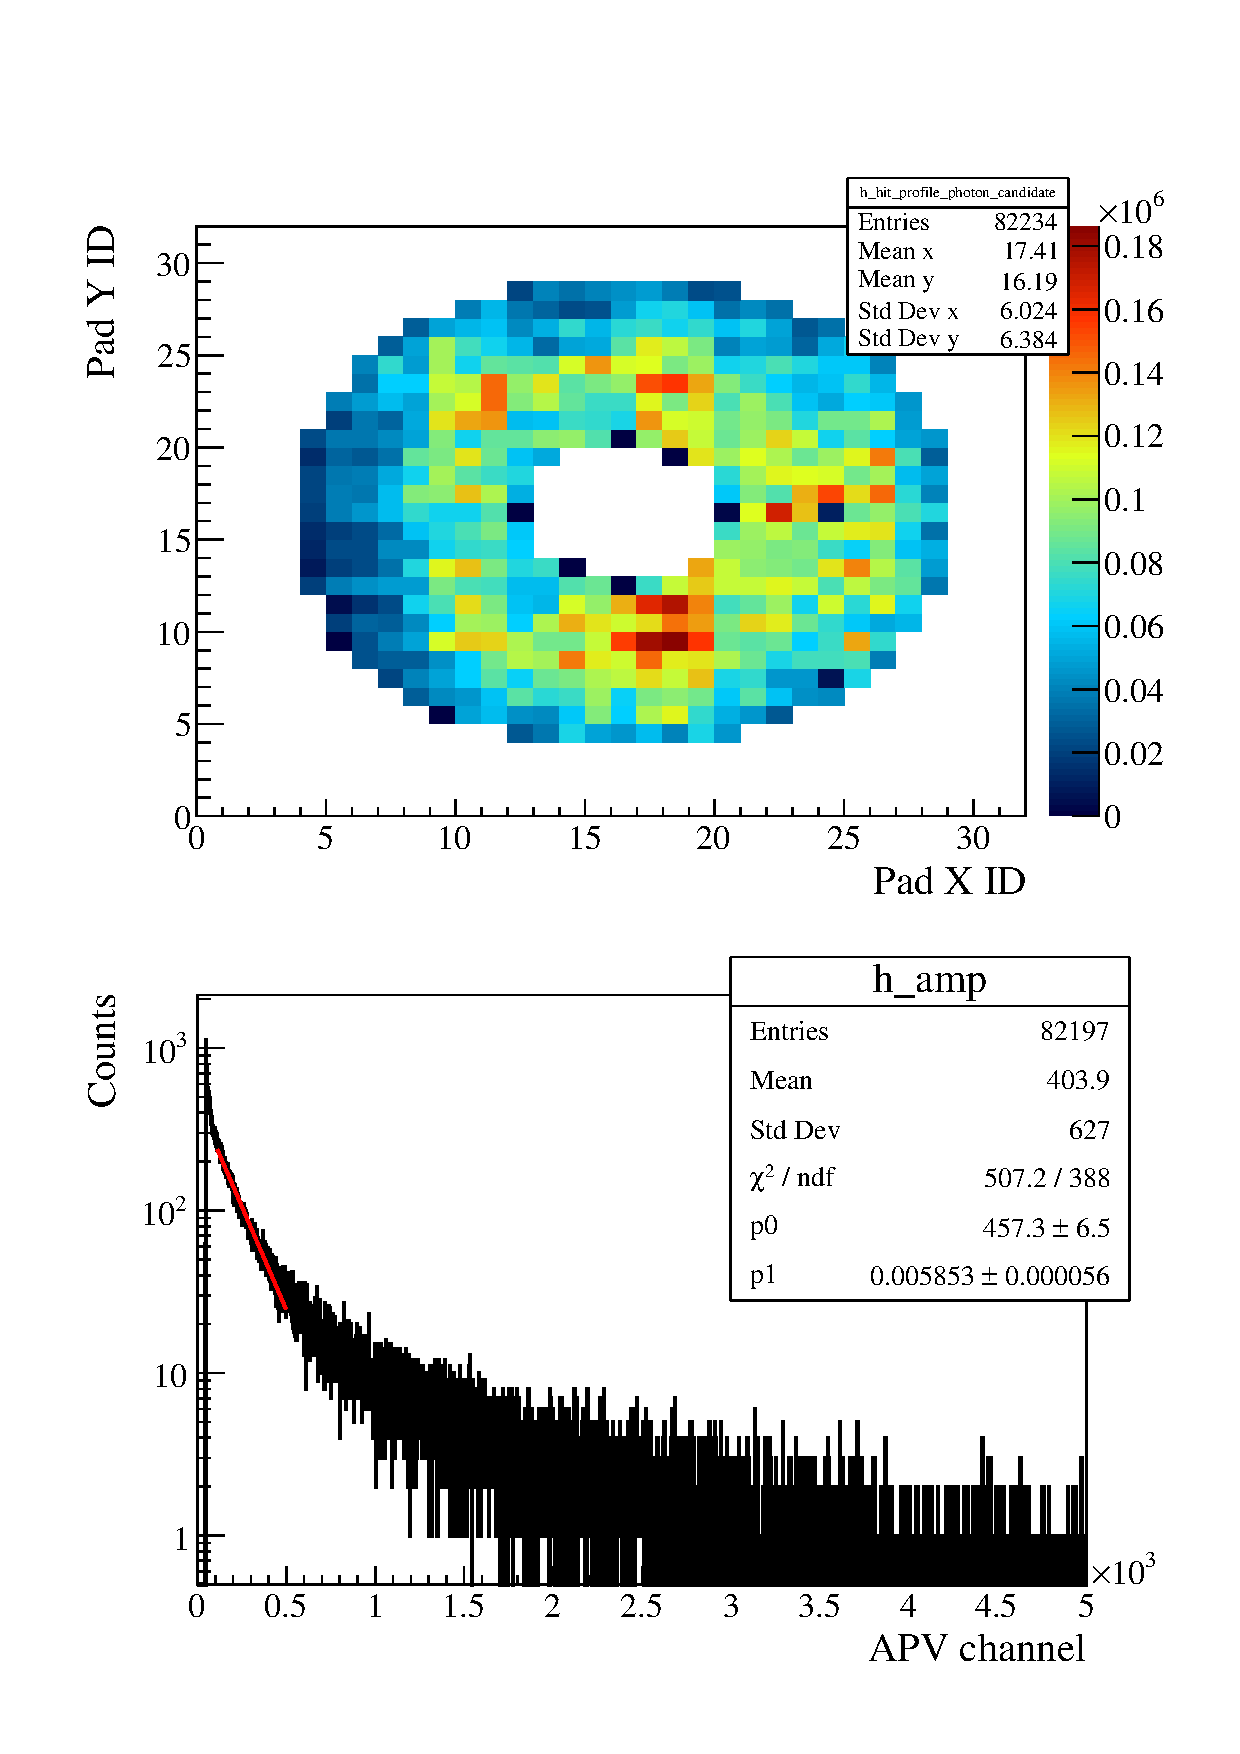
\includegraphics[width=0.6\textwidth]
                			{INFN_plots/cluster_gain_fit}
				\caption{\label{fig:cluster_gain_fit}
               Events collected with the shutter between the radiator and the photocathode open. top) 2-D histogram indicating the ring area. bottom) Amplitude spectrum of the reconstructed clusters in the ring area; the spectrum is fitted to an exponential function, where the inverse of the slope represents the mean amplitude in ADC channels. }
			\end{center}
            \end{figure} 
            %%%%%%%%%%%%%%%%%%
     \par
     The analysis of the test-beam data is in a very initial stage and has to be continued and improved in the coming months. Nevertheless, the first indications are very positive: the prototype has successfully detected single photons and it has been operated at large gain.
\item
Initial studies to understand the 
compatibility of an \textbf{innovative photocathode 
based on NanoDiamond (ND) particles} with the 
operation in gaseous detectors and, in 
particular, in MPGD-based photon detectors\\
The results of the characterization of the first THGEMs 
coated with ND powder have been reported in July 2018. 
An aspect is surprising and puzzling: the THGEMs with
ND powder coating exhibit 
higher gain for a given biasing voltage respect 
to the gain measured for 
the same THGEM before applying the coating.
The characterization measurements have been repeated, confirming 
the result, while a possible explanation is emerging.
The coating layer is resistive and it covers both the 
metallized part and insulating part of the THGEM. 
Therefore, its presence can prevent
 the charging up of the insulating surfaces. 
It is expected that the THGEM multiplication is 
higher when there is no charging up. This hypothesis 
has to be supported by further measurements. 
\par
In parallel, in order to prepare further studies, actions towards material procurement 
are taking place, 
both concerning new ND powder samples and more small-size THGEMs.
\end{enumerate}    
\par
Concerning the \textbf{dissemination of the results}:
\begin{itemize}
\item The initial results concerning the performance of the photon
detector prototype with miniaturized pads have been present at 
\textbf{the 
14$^{th}$ Pisa Meeting on Advanced Detectors},
La Biodola, Isola d'Elba (Italy), 27 May - 02 June 2018,
\cite{AGARWALA2018-2} and at \textbf{the 
10th International Workshop on Ring Imaging Cherenkov Detectors}, 
Moscow (Russia) 29 July – 4 August 2018.
\item The first studies concerning the coupling of ND photocathodes and MPGDs have been presented at \textbf{the 
10th International Workshop on Ring Imaging Cherenkov Detectors}, 
Moscow (Russia) 29 July – 4 August 2018\cite{Agarwala:2018qdm} \end{itemize}
\end{itemize}
\par
Concerning the 
\textbf{milestones for 2018}:
\begin{itemize}
\item
\textbf{September 2018: The completion of the laboratory 
characterization 
of the photon detector with miniaturized pad-size.}\\
The exercise has been completed and the milestone is
successfully matched.
\item
\textbf{September 2018: 
The performance of the tests to establish the 
compatibility of the ND photocathodes with the
operation of MPGD-based photon detectors.}\\
The tests have been performed and, therefore, the
milestone is partially matched. Nevertheless, there is
not yet a solid answer to the question related to the
compatibility:  
the totally
unexpected results demand 
for further investigation in 2019.
\end{itemize}
\subsubsection{Stony Brook University}  
\paragraph{Ion Back Flow} A TPC prototype has been constructed and a sophisticated test-beam setup established. We purchased picoammeter from PicoLogic in Zagreb/Croatia which is a unique device that allows to measure very small currents at high potential. The floating current measurements can be performed at potentials much larger than 5 kV, ideally suited for IBF measurements in a TPC.

The TPC prototype has been equipped with a real size readout module, based on a quadruple-GEM stack similar to the ALICE-TPC readout and zig-zag pad readout structure. The prototype has been exposed to the 120 GeV protons at the Fermilab Test Beam Facility (FTBF) to establish the working parameters of the TPC. We have analyzed the data obtained from the test-beam campaign and verified the performance parameter of the prototype. The resolution has been obtained by measuring with a drift-length of 40 cm at B = 0 T and extrapolated to the magnetic field with the Babar magnet at B = 1.4 T with \[\sigma^2_{total}=\sigma^2_{int}+\frac{D^2_TL}{N_{eff}}+\sigma^2_{sc}\]
with $\sigma_{int}=\sigma(z=0)$: intrinsic resolution, $D_T$: diffusion constant, $L$: drift length, $N_{eff}$: effective number of electrons leading to the readout signal and $\sigma_{sc}$: smearing due to space charge distortions. The smearing due to space charge distortions can be neglected at the test-beam. The measurement/extrapolation principle can be taken from Fig.~\ref{fig:measPrinc}.
\begin{figure}
    \centering
    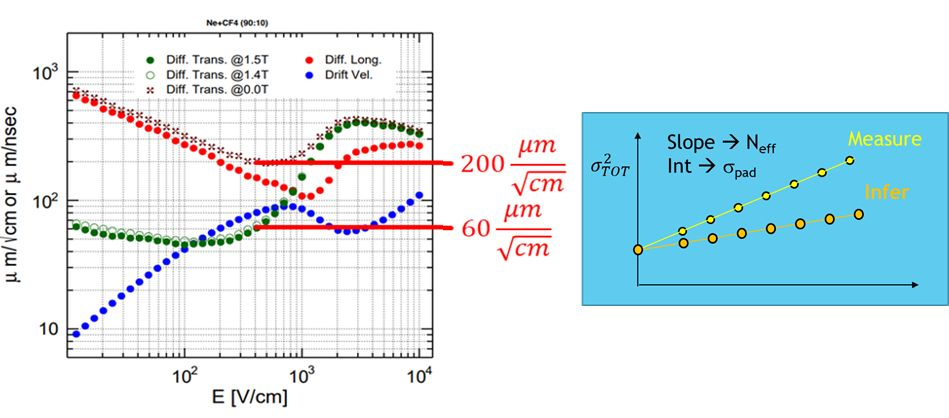
\includegraphics[width=\columnwidth]{SBU_plots/TPCresolutionPrinciple.jpg}
    \caption{\label{fig:measPrinc}Principle for the determination of space point resolution at B = 0 T and extrapolation to B = 1.4 T.}
\end{figure}
The results for this procedure are shown in Fig.~\ref{fig:TPCres}.
\begin{figure}
    \centering
    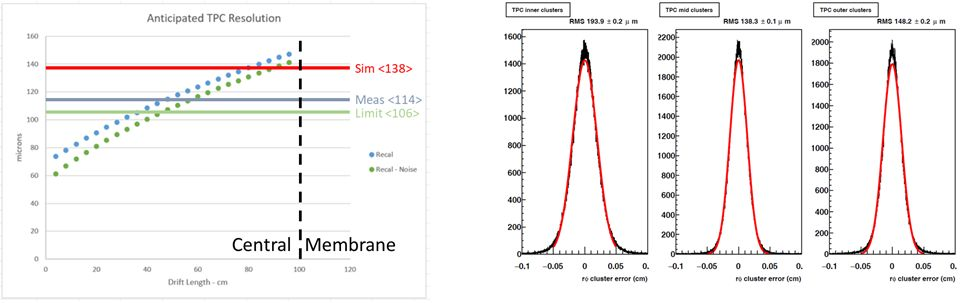
\includegraphics[width=\columnwidth]{SBU_plots/TPCresolution.jpg}
    \caption{\label{fig:TPCres}Comparison of measured (left) and simulated (right) space point resolution.}
\end{figure}

\paragraph{Mirror coating} We have continued to install components of the electron-/ion-gun for the evaporation of thin layer structures on mirror surfaces. The installation is running smoothly and undergraduate students are gaining experience in handling the sensitive equipment under the supervision of senior personnel. The installation process also helps in understanding the equipment and in preparing the start-up procedure of operation.

\paragraph{Meta-materials}
We have started evaluating procedures of transformation optics with which one can obtain properties of materials that allow to modify the Cherenkov angles but maintaining the momentum reach for high momentum particles. Based on the dispersion relation (from \cite{Vginis:2014})
\[\frac{k_x^2}{f'^2(x)}+\frac{k_y^2}{g'^2(y)}+\frac{k_z^2}{h'^2(z)}=\epsilon_b\frac{\omega^2}{c^2}.
\]
and substituting $f'(x)=F~(=\frac{\partial x}{\partial x'}),~g'(y)=G~(=\frac{\partial y}{\partial y'}),~h'(z)=H~(=\frac{\partial z}{\partial z'})$ we were able to reproduce the simulated results obtained in \cite{Vginis:2014}, Figs.~1 a) and b). These reproduced results can be seen in Figs.~\ref{fig:phiVsF}, \ref{fig:phiVsG}.

\begin{figure}
    \centering
    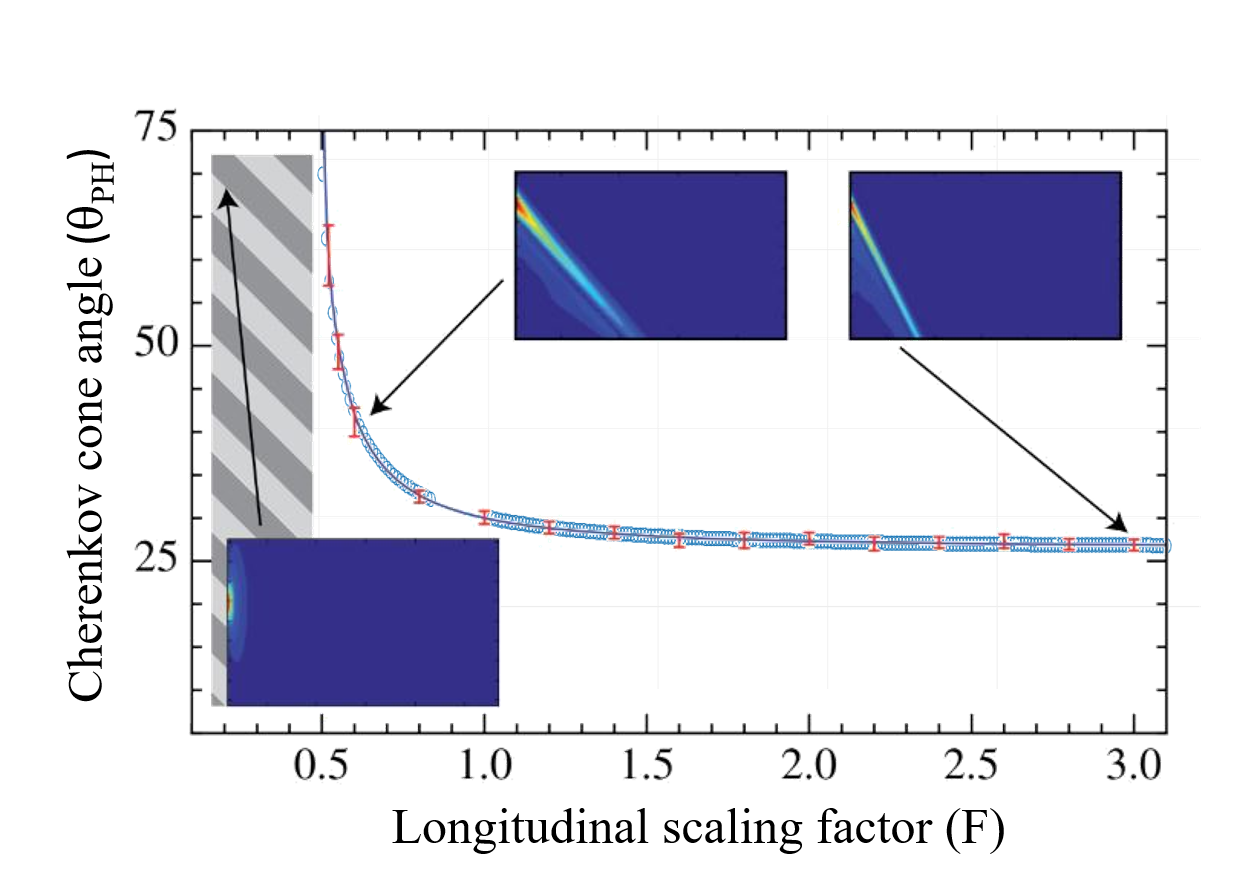
\includegraphics[width=0.8\columnwidth]{SBU_plots/phiVsFoverlayed.png}
    \caption{\label{fig:phiVsF}Data reproduction (open blue circles) based on the calculations obtained from the transformation optics overlaid on \cite{Vginis:2014} Fig.~1a).}
%\end{figure}
%\begin{figure}
%    \centering
    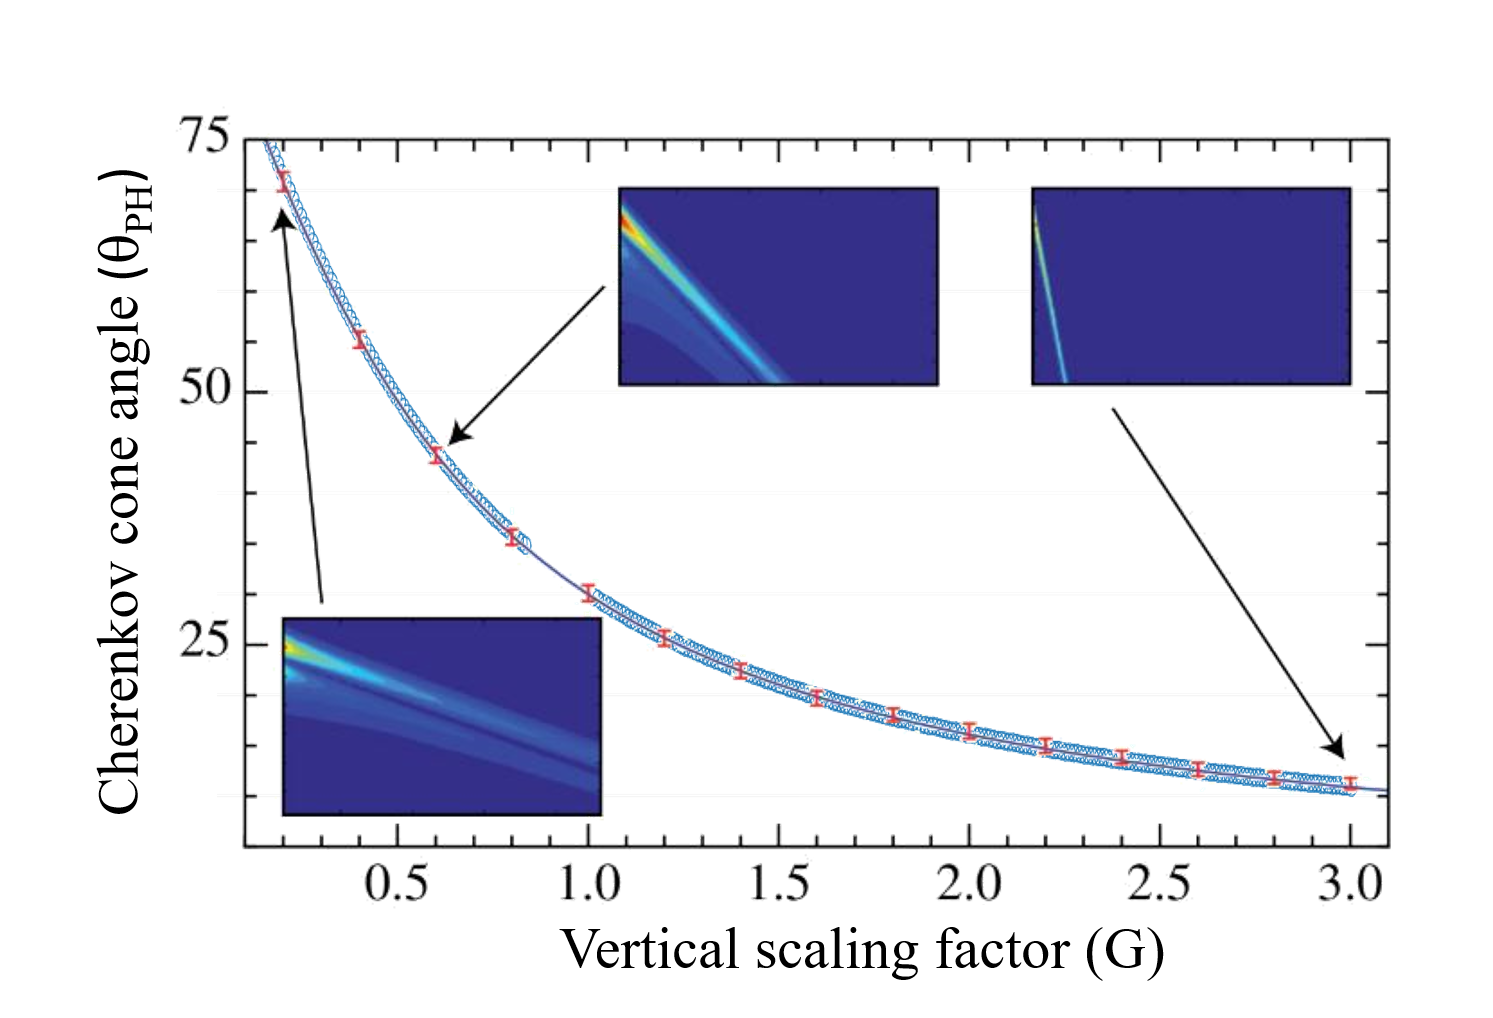
\includegraphics[width=0.8\columnwidth]{SBU_plots/phiVsGoverlayed.png}
    \caption{\label{fig:phiVsG}Data reproduction (open blue circles) based on the calculations obtained from the transformation optics overlaid on \cite{Vginis:2014} Fig.~1b).}
\end{figure}
\subsubsection{Temple University} 
\paragraph*{Commercial Triple-GEM Detectors}\mbox{}\\
Temple University was able to achieve several goals that were set for this funding cycle. 
Last summer two commercial triple-GEM detectors were built, one using Kapton rings as the spacers between the GEM layers and another using more traditional G10 spacer grids. Upon completion of the two triple-GEM detectors, they were inserted into the cosmic ray test bench where both detectors drew about twice as much current as the STAR FGT triple-GEM detectors, and exhibited excessive sparking. This sparking ultimately led to both detectors failing and becoming unusable. After opening the detectors and inspecting the layers, the effects of excessive sparking were clear, as can be seen in fig.~\ref{fig:spark}. It was hypothesized that the sparking was a result of shorts originating in the HV connector pads on the GEM foils in each layer. Each GEM foil is segmented into nine HV sectors on one side, while the other side is unsegmented. Each of the nine HV sectors connects to three HV pads located at the top of the GEM foil. Additionally, there are three pads which connect to the unsegmented side of the GEM foil, as shown in fig.~\ref{fig:EICFGT}. The HV pin connections are then made to a HV pad position that is associated with one of the three triple-GEM layers, \emph{e.g.} the middle GEM foil layer has HV pins connected to the HV pads in the center of the three pads for each sector. In the initial two triple-GEM detectors built, the unused HV pads for each GEM foil layer were left in tack with the thinking that the pins passing through the unused HV pads would be isolated from them since they are not physically touching the HV pads. However this turned out not to be the case and was found to be the cause of the shorts in the initial commercial triple-GEM detectors. This was verified during the building of the third commercial triple-GEM detector. After stretching and gluing all foils to their respective frames, the triple-GEM stack was assembled by simply stacking the various layers without glue. We then tested the detector for shorts amongst the HV pins, where we were able to generate shorts with minor movements of the HV pins. The stack was then disassembled and all unused HV pads on each GEM foil were cut away. The detector stack was reassembled and tested again for shorts. With the excess HV pads removed we were not able to detect any shorts. Gluing the stack of the third commercial GEM detector and inserting it into the cosmic ray stand, we now see the same current being pulled as that STAR FGT triple-GEM detectors pull. This suggests that the shorting issue that plagued the first two triple-GEM detectors is now solved.      

Now that the shorting issue has been resolved we are ready to begin the characterization of the triple-GEM detector. Figure~\ref{fig:EICGFTcosmic} shows initial reconstructed cosmic ray hits.
There is enough material remaining to assemble a fourth commercial triple-GEM detector. The GEM, readout, and HV foils for this detector have now been stretched and glued to their respective frames. The assembly of the GEM stack was delayed until we saw how the third triple-GEM detector performed, in case we needed to correct any unforeseen issues.

\begin{figure}
\center
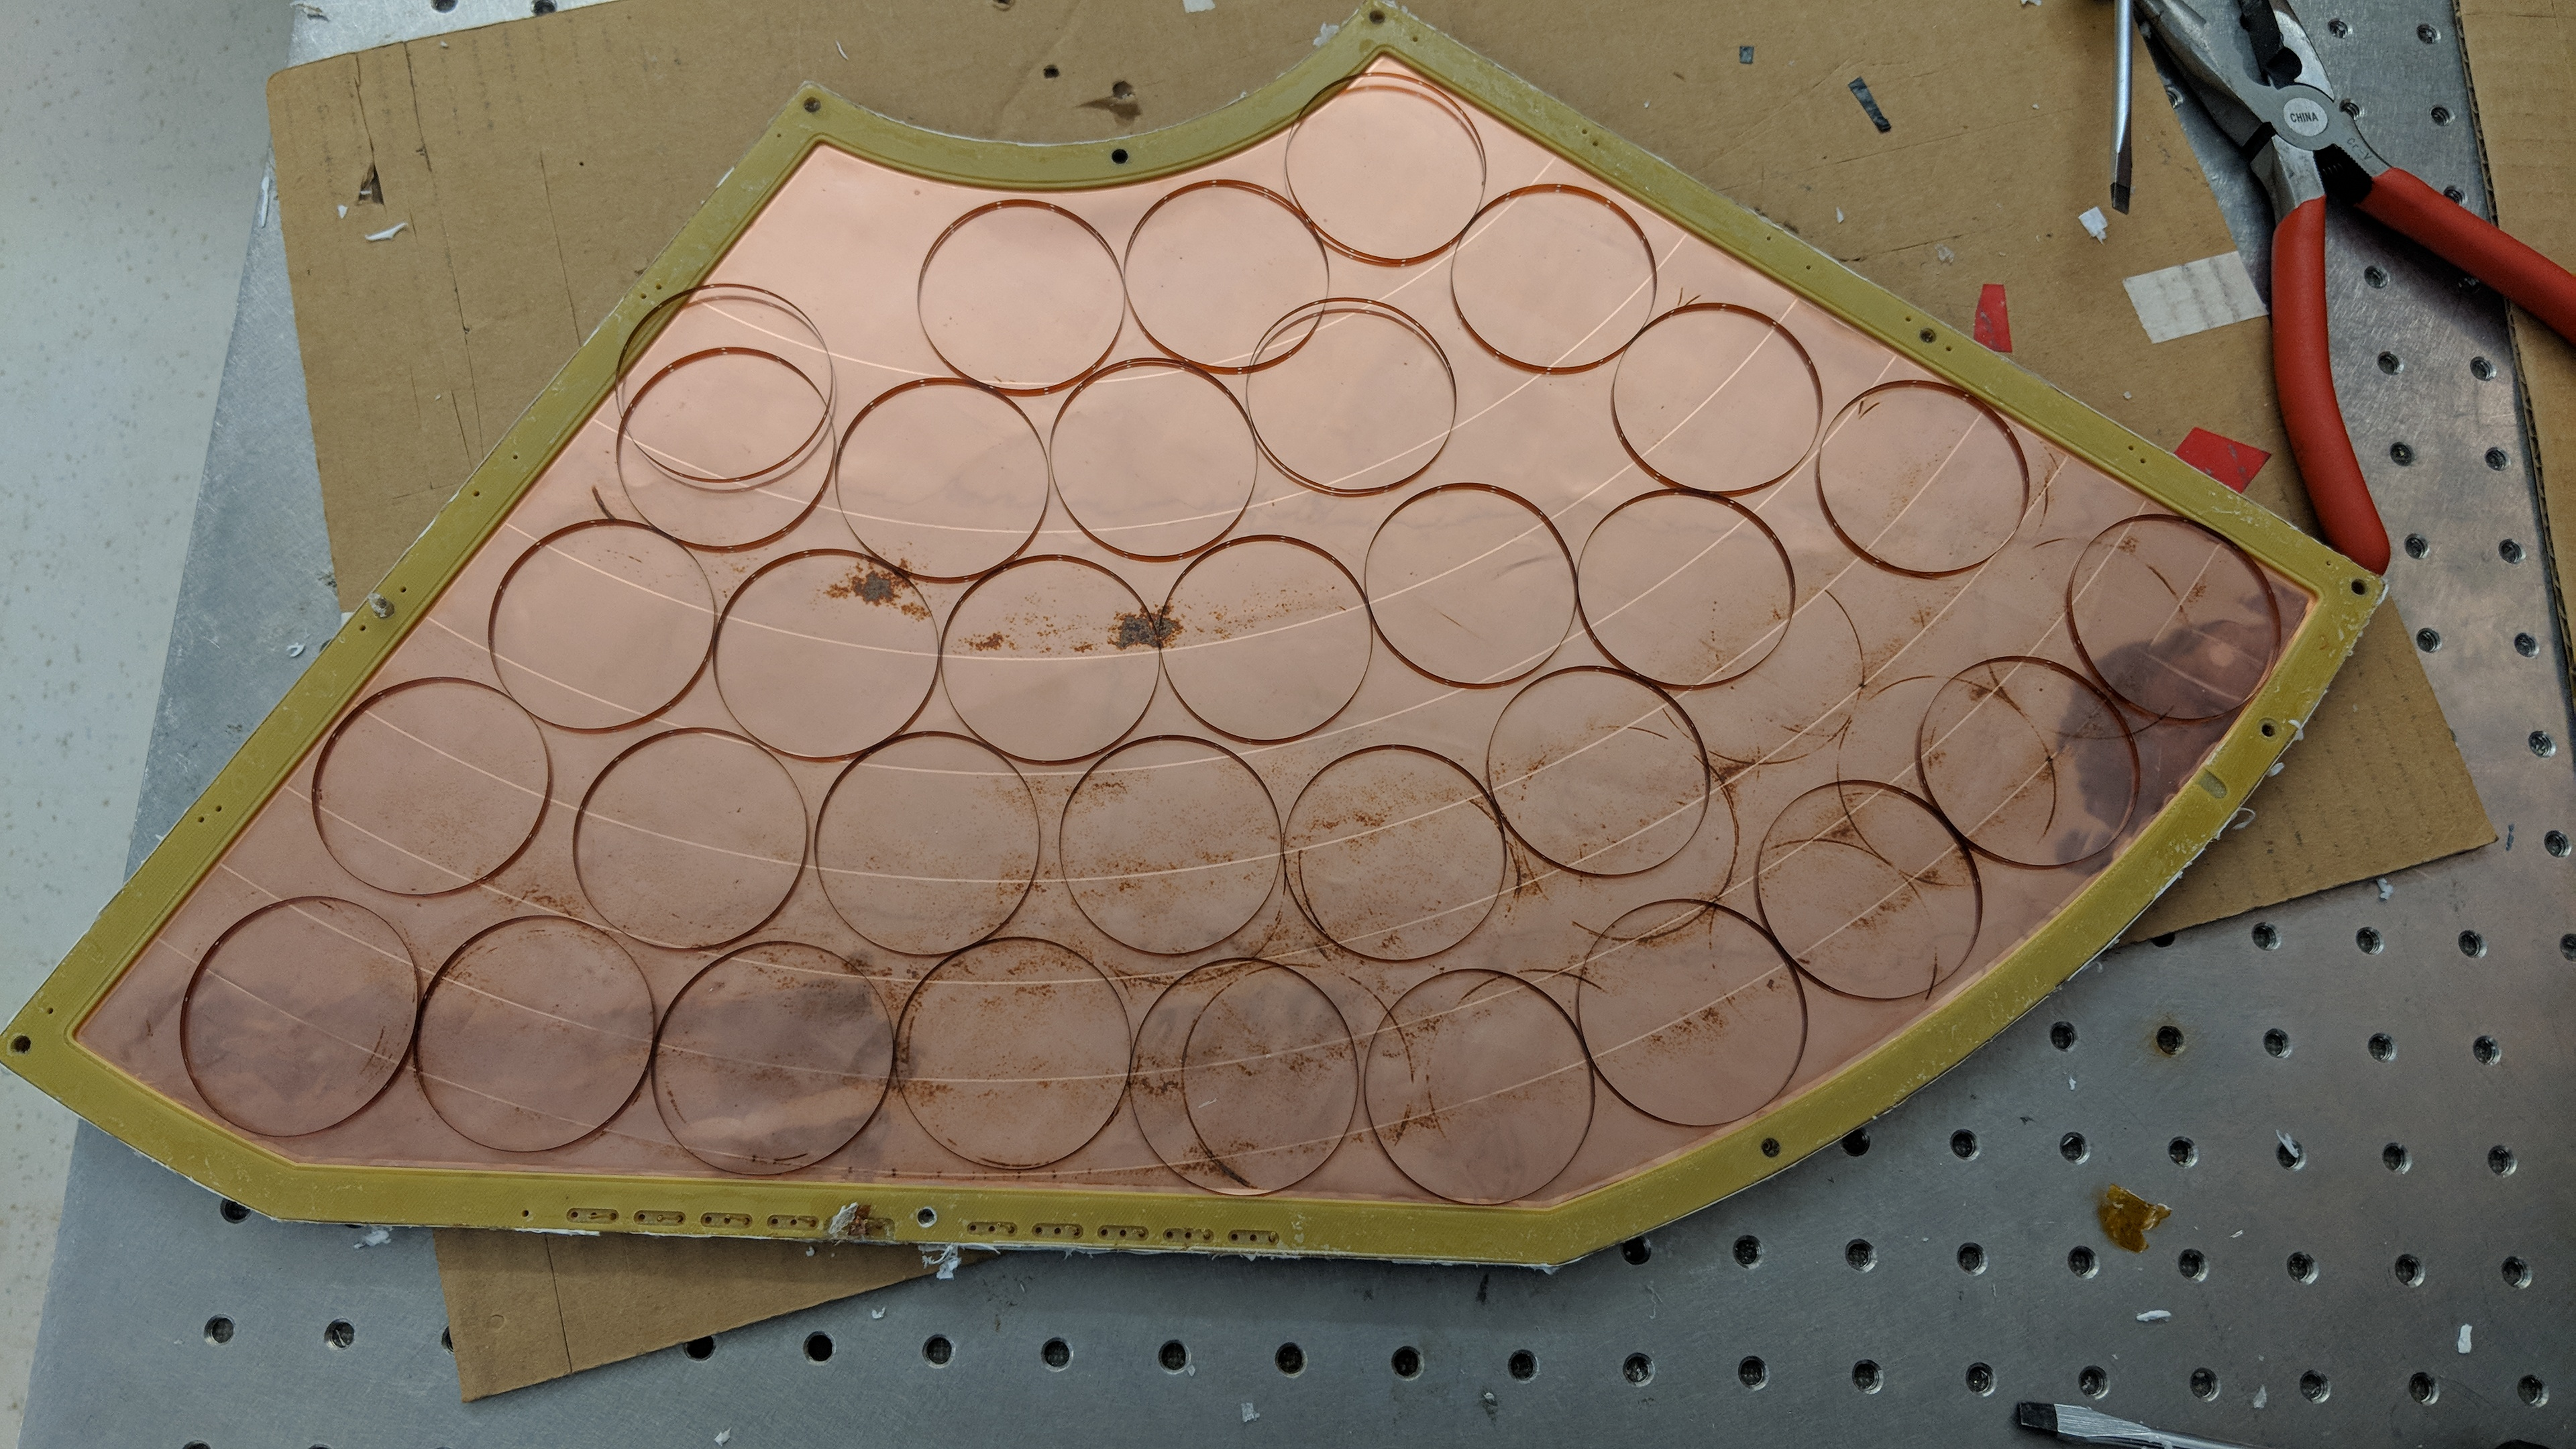
\includegraphics[width=\columnwidth]{TU_plots/GEM-spark.jpg}
\caption{\label{fig:spark}Damage to a GEM layer in the first commercial triple-GEM detector caused by excessive sparking resulting from electrical shorts.}
\end{figure}


\begin{figure}
\center
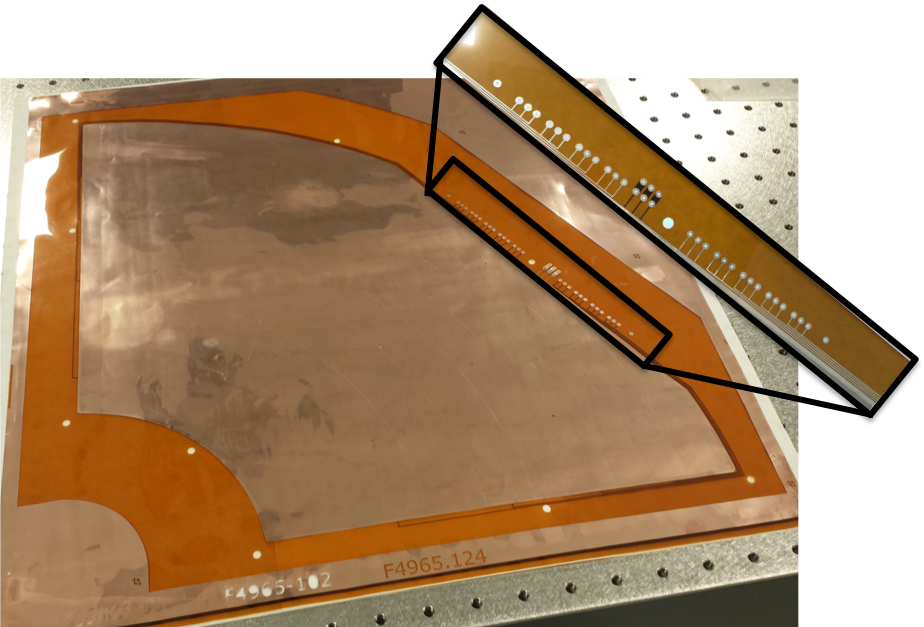
\includegraphics[width=\columnwidth]{TU_plots/GEM-HVPad.png}
\caption{\label{fig:EICFGT} Commercial GEM foil HV sectors and connection pads.}
\end{figure}

\begin{figure}
\center
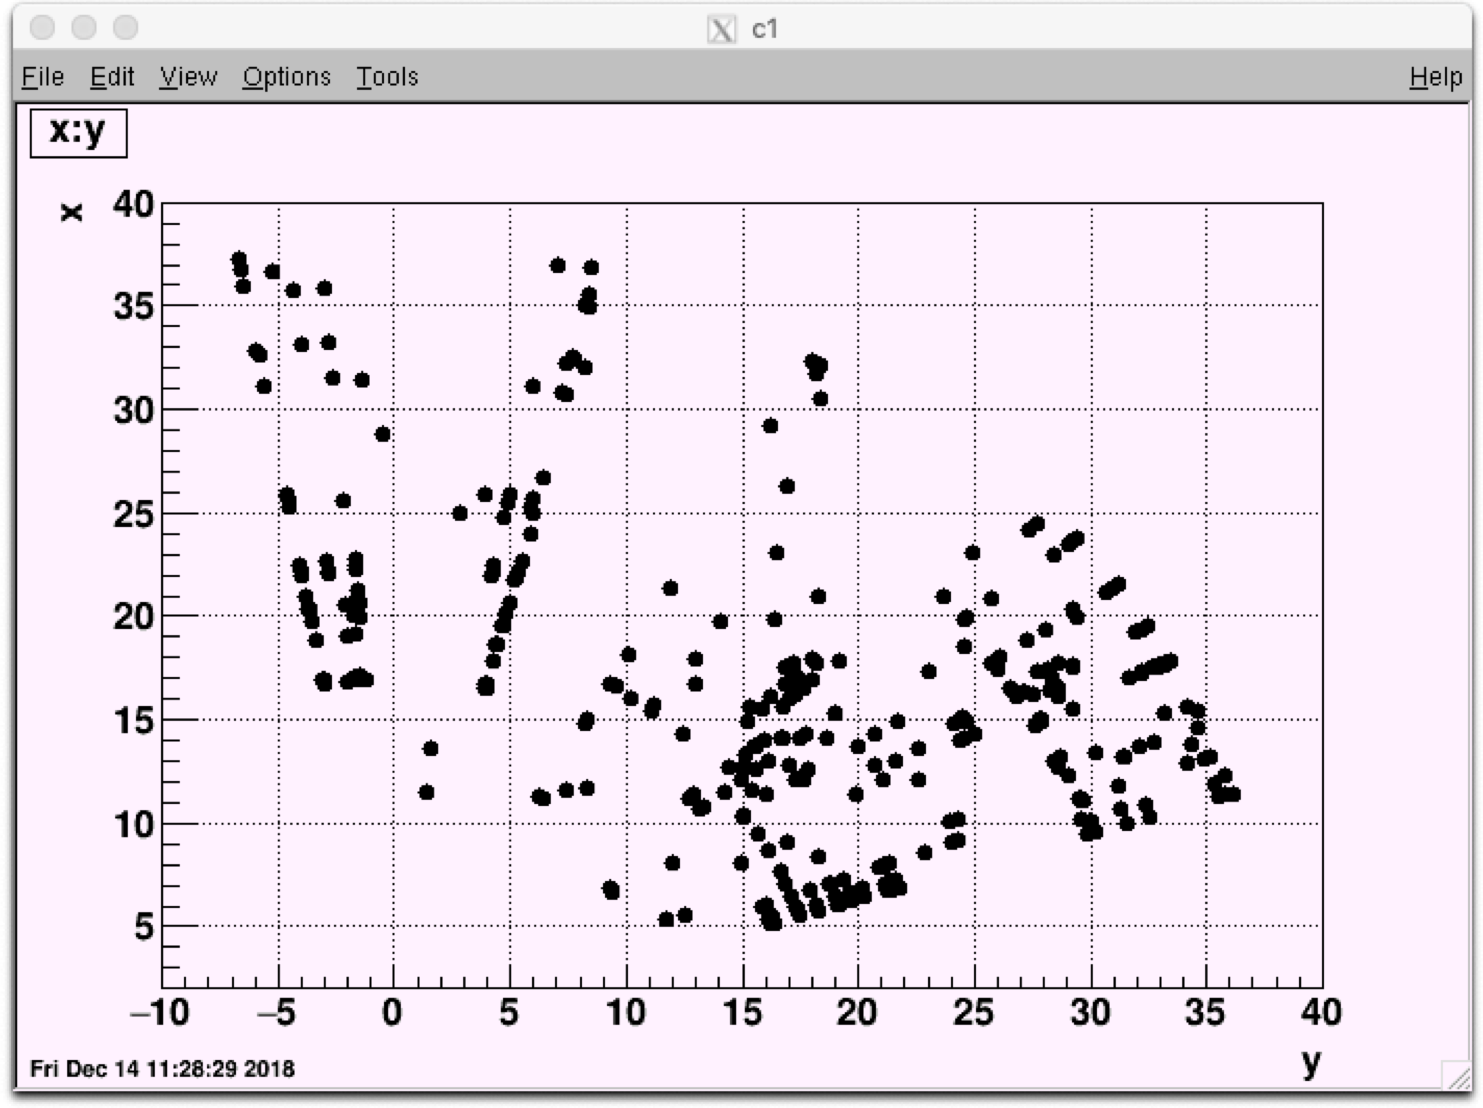
\includegraphics[width=\columnwidth]{TU_plots/Cosmic.png}
\caption{\label{fig:EICGFTcosmic}Commercial triple-GEM detector showing reconstructed X-Y hit of cosmic ray events.}
\end{figure}

\paragraph*{MPGD $\mu$TPC Simulation}\mbox{}\\
In addition to the hardware work, we are also working on some simulations. The initial machinery needed to produce a MPGD detector in $\mu$TPC mode has now been implemented. This machinery allows one to create a barrel geometry with a specified dead material radiation length and drift gap filled with a particular gas. This machinery also allows one to simulate multiple hit points by defining sensitive barrel layers within the drift gap volume. The resolution parameters of the detector are also adjustable. For example one can specify the detectors radial and transverse resolutions, as well as its hit point resolution. This machinery has now been tested using some nominal settings and is currently being modified to reflect more realistic parameters and digitization.
\subsubsection{University of Virginia} 
%
\paragraph*{Large EIC GEM prototype with 2D U-V strip readout}%\mbox{}\\
\subparagraph*{\textbf  Characterization with Cosmics:}
% 
\begin{figure}[htb]
\centering
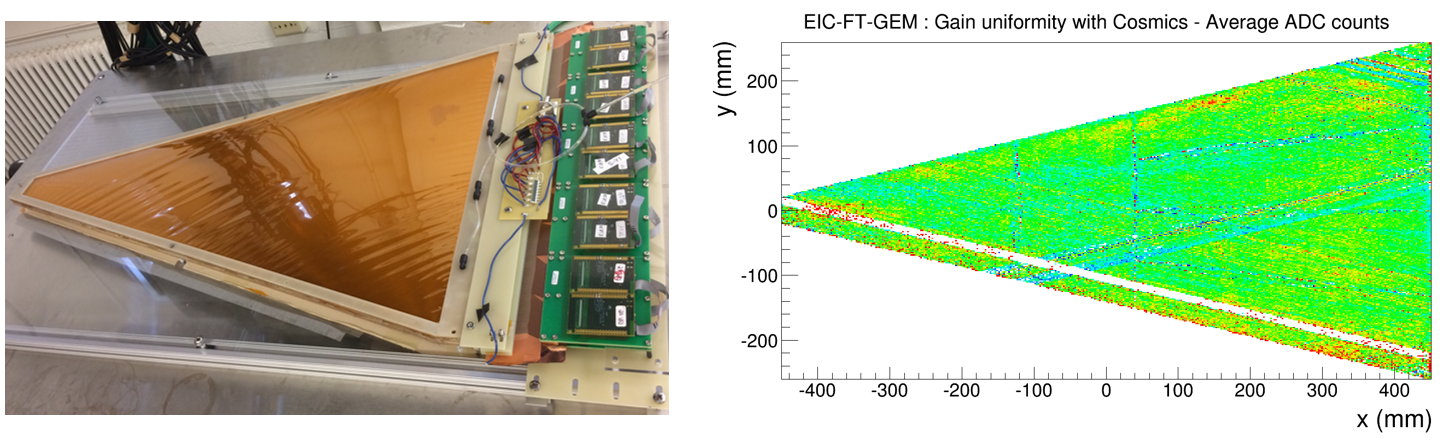
\includegraphics[width=1\columnwidth,trim={0pt 0mm 0pt 0mm},clip]{UVa_plots/eicCosmics}
\caption{\label{fig:eicCosmics}({\it Left:}) UVa large GEM prototype on the cosmic bench at UVa;  ({\it right:}) Gain uniformity: Distribution of the average charge in ADC counts.}
\end{figure}
%
Preliminary tests of the large EIC GEM prototype with cosmics showed a detector gain about an order of magnitude lower than the expected gain of ~8000 of a typical triple-GEM operating with Ar-CO2 (70/30) mixture at the nominal voltage 4.1kV. A likely explanation of the lower gain can be a explained by GEM hole geometry from the production batch for our foil, slightly different from  bi-conical (70-50-70 $\mu$m) shape  of the holes of standard GEM foils. In this case, even a relatively modest gain drop per GEM foil results to a significant gain drop in a triple-GEM detector configuration. Increasing the voltage on the divider from 4.1kV to 4.3kV was enough to restore the nominal operating gain. However, due the large detector size and various challenges related to the  stretching of the GEM foils during the assembly, we could not operate the detector in a stable way at 4.3kV. We therefore decided to test the prototype with Ar-CO2 (80/20) mixture instead of Ar-CO2 (70/30) which allow us to operate at a gain of $\sim 10^4$  at 4.1kV. The prototype was then characterized with cosmics for a three weeks period during which we collected 4  million triggered cosmic events. Fig.~\ref{fig:eicCosmics} ({\it top left}) shows the detector on the cosmic stand in the Detector Lab at UVa.  The plot on {\it top right}, shows a fairly uniform distribution of the average ADC (ratio of the total accumulated charge over the number of hits per unit area)  across  the entire active area for 4 millions cosmic events. This is gain uniformity performance of the chamber. The efficiency drop caused by the presence of GEM support spacers can clearly be seen as well as dead area due to a few broken strips.  The overall uniform gain distribution successfully demonstrates that the novel double-sided zebra connection system that we developed for the readout electronics works perfectly as expected. Analysis of the cosmic data is ongoing.
%
\subparagraph*{\textbf Characterization of UVa large GEM prototype in test beam at FNAL:}
%
\begin{figure}[htb]
\centering
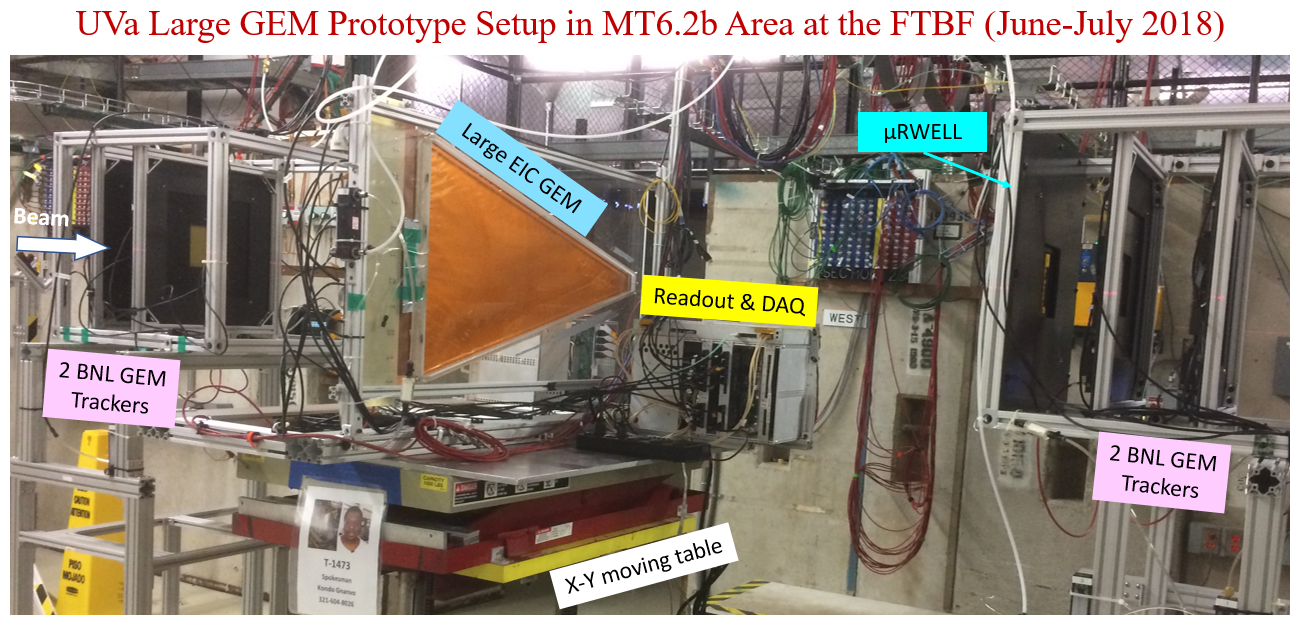
\includegraphics[width=1\columnwidth,trim={0pt 0mm 0pt 0mm},clip]{UVa_plots/ftbfSetup}
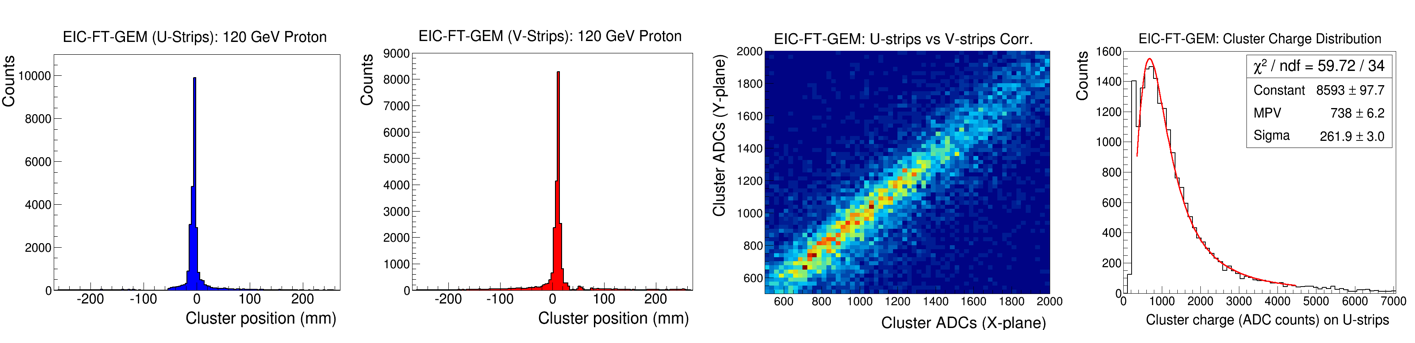
\includegraphics[width=1\columnwidth,trim={0pt 0mm 0pt 0mm},clip]{UVa_plots/eicProtonBeam}
\caption{\label{fig:eicProtonBeam} \textit{Top:} Large GEM setup at FNAL FTBF with two BNL GEMs for the upstream telescope and two other and the  small $\mu$RWELL prototype for the downstream telescope. \textit{Bottom:} Characteristics of the prototype; \textit{Left to right:} 120 GeV proton beam profile on U-strips and V-strips; Charge sharing correlation between the top (U-strips) and bottom (V-strips); Charge distribution in ADC counts on U-strips.}
\end{figure}
%
The large EIC GEM prototype, together with the small $\mu$RWELL prototype and an additional small triple-GEM with 2D zigzag strip prototypes were brought to the Fermilab Test Beam Facility (FTBF) this summer (June 2018 - July 2018) and tested with the 120 GeV primary proton beam  for a period of 3 weeks.
% The beam test campaign was a combined effort which includes M. Hohlmann's group  from Florida Tech (FIT), also testing  their large EIC GEM prototype with zigzag strip readout and K. Dehmelt and T. Hemmick's group from Stony Brook (SBU) testing their small TPC prototype with GEM readout. UVa and FIT shared the same large EIC GEMs setup with the prototypes installed on the X-Y moving table of the  MT6.2b area at the FTBF.
For the tracking, our colleagues from BNL group provided four small triple-GEMs COMPASS readout. The setup is shown on Fig.~\ref{fig:eicProtonBeam} with  BNL GEM trackers and the $\mu$RWELL prototype used as upstream and downstream telescopes. The detector configuration in the setup  was optimized to minimize the  multiple scattering impact on the resolution studies of the EIC GEM prototype. All chambers, including the four BNL GEM trackers operated with the same Ar-CO2 (70/30) gas mixture and the APV25-based Scalable Readout System (SRS) electronics developed at CERN by the RD51 collaboration were used to read out all chambers channels at a trigger rate of $\sim$ 400Hz with the trigger signal from the facility scintillators/PMTs. DATE and AMORE, developed by the CERN ALICE experiment, where used respectively as DAQ software and online/offline  analysis tool.\\
 The plots on the left of Fig.~\ref{fig:eicProtonBeam} show the 120 GeV proton beam profile reconstructed respectively on the top (U-strips) and bottom layers (V-strips) of the U-V readout foil.  Plot on center right shows the excellent correlation of the charges (in ADC counts)  shared between U-strips and V-strips. The  charge distribution (in ADC counts) of the top layer (U-strips) is shown on the right plot. The distribution fits nicely with the Landau function as expected from minimum ionizing particles. This new U-V strips readout foil design developed for this prototype is a clear improvement of the previous iteration that was tested in our  first large EIC GEM prototype in 2013 \cite{Gnanvo:2015xda}. 
%
\subparagraph*{\textbf Issues with the U-V strips readout quality:}
%
\begin{figure}[htb]
\centering
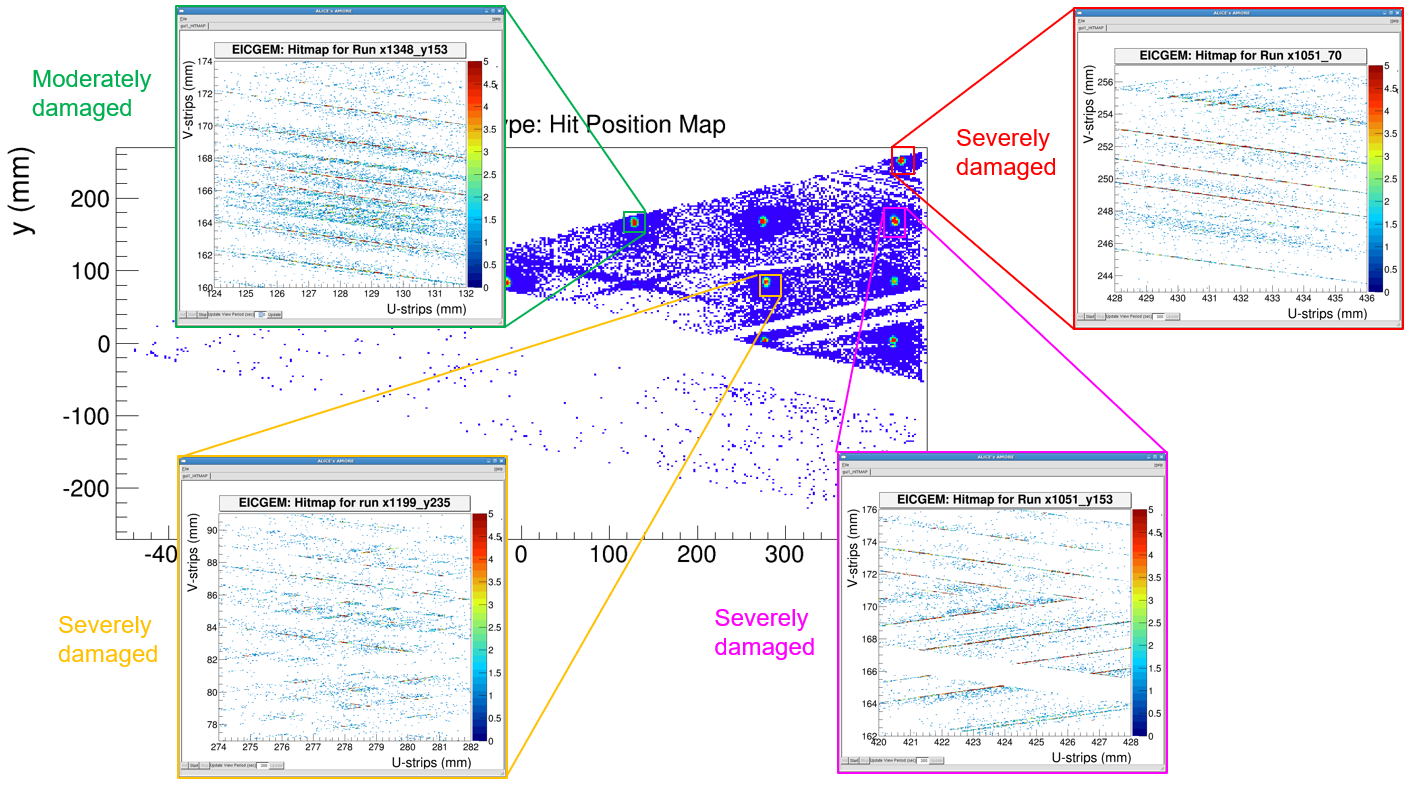
\includegraphics[width=1\columnwidth,trim={0pt 0mm 0pt 0mm},clip]{UVa_plots/eicPosScan}
\caption{\label{fig:eicPosScan}  2D  reconstruction of 120 GeV proton beam from position scan in the top half of the EIC GEM prototype. A zoom in of  reconstructed particle positions for at four beam spots showing some unexpected patterns of non uniform distribution of the reconstructed particle positions likely due to poor production quality of the readout strip layer.}
\end{figure}
%
Fig.~\ref{fig:eicPosScan} shows the 2D reconstruction of the proton beam from a position scan run. A detailed analysis with a fine histogram binning of the area around the beam spot reveals some unexpected patterns of reconstructed positions as can be seen on the four "zoom-in" locations on Fig.~\ref{fig:eicPosScan}. Instead of a uniform distribution of the reconstructed points, what we actually observed  is a picture of  the reconstructed positions heavily concentrated along a set of lines parallel to the strips. As indicated on the plots, the pattern of the reconstructed positions are more pronounced \textit{\textbf{``severe distorsions''}} in some locations than other \textit{\textbf{``moderate distorsions''}} but seems to be present anywhere where we were able to collect data from. These patterns suggests that a significant number of the strips could be shorted both on top and bottom strip layers. A few consecutive shorted strips will destroy the advantage of using  the center of gravity method  to reconstruct the position with high precision and results in the positions reconstructed at the physical center of a single strip and the pattern of highly concentrated parallel lines that we observe in the plots. We are not however completely discarded the possibility that some issues inherent to the zebra strips technology we are using to interface the readout strips to the FE electronics might be the source of distorted signal at the input of the FE readout channels and degrades the position information. We are investigating the  problem with ongoing tests and analysis.
%
\subparagraph*{\textbf Position residual distribution:}
%
\begin{figure}[htb]
\centering
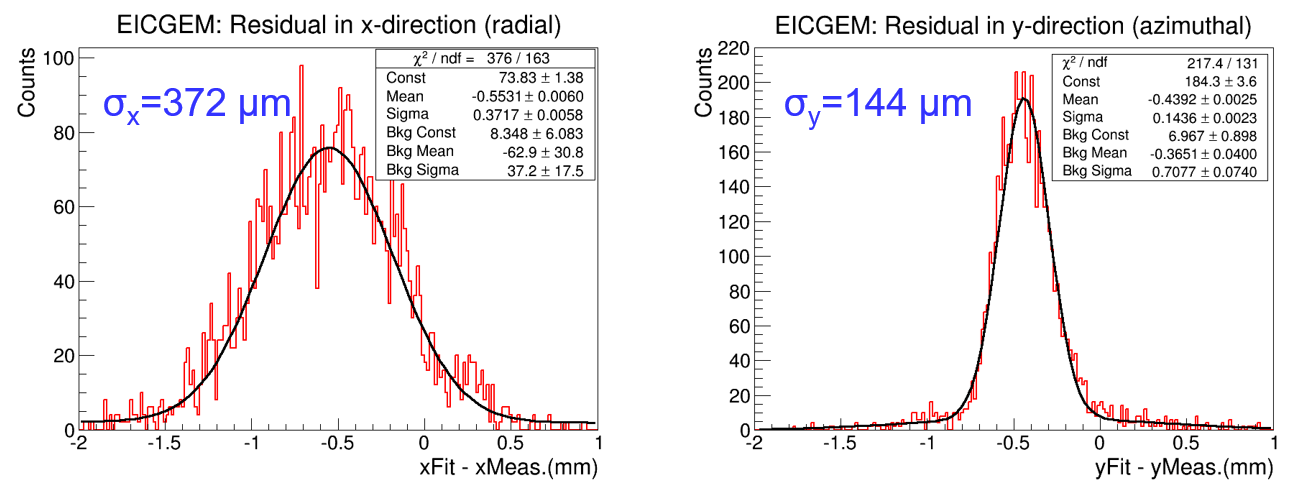
\includegraphics[width=1\columnwidth,trim={0pt 0mm 0pt 0mm},clip]{UVa_plots/eicResidual}
\caption{\label{fig:eicResidual} Residual distribution in x {\it(left:)} and y {\it (right:)} from the proton beam at two locations on the large GEM prototype:  moderate strip distortions area {\it (top plots)} and  severe strip distortions area {\it (bottom plots)} on the large GEM prototype.}
\end{figure}
%
\paragraph*{$\mu$RWELL  prototype with 2D X-Y strip readout}\mbox{}\\
\subparagraph*{\textbf Characterization with Cosmics:}
%
\begin{figure}[htb]
\centering
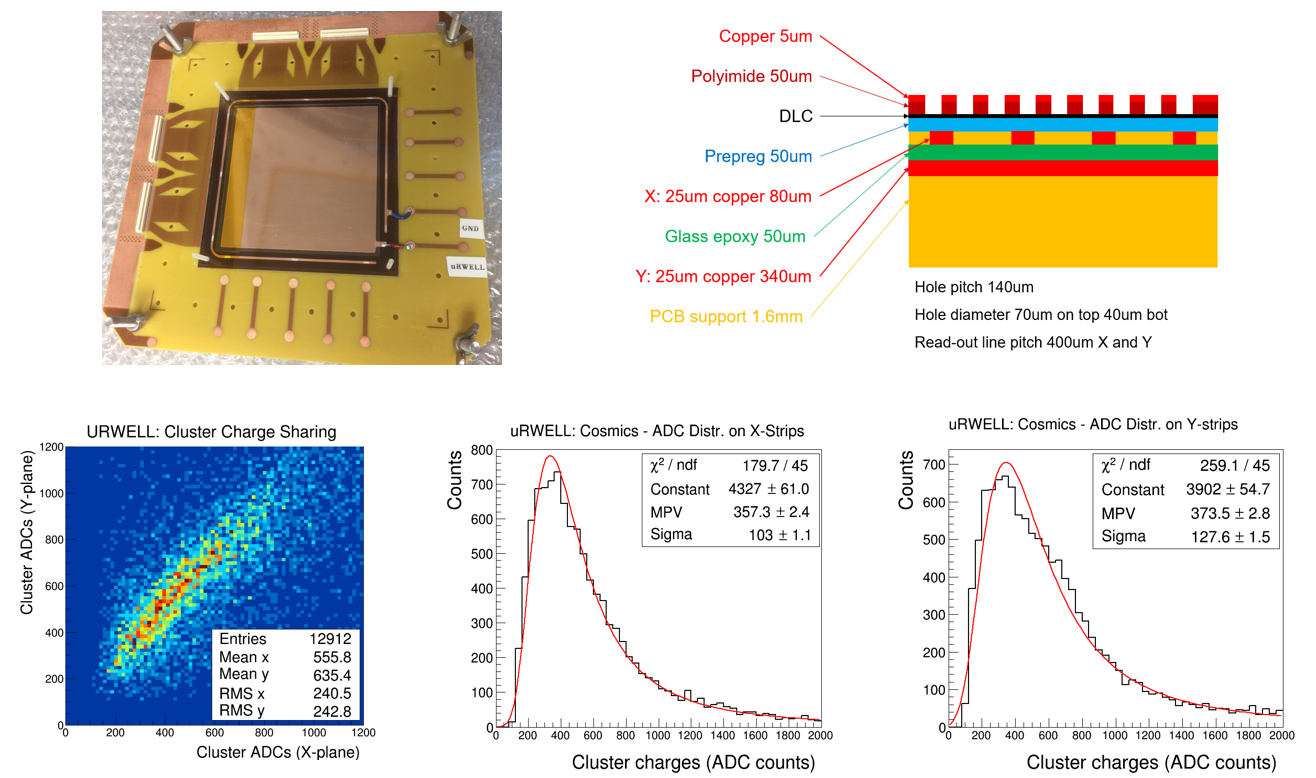
\includegraphics[width=1\columnwidth,trim={0pt 0mm 0pt 0mm},clip]{UVa_plots/uRwellCosmics}
\caption{\label{fig:uRwellCosmics} The $\mu$RWELL prototype with 2D X-Y readout strip, the cross section of the detector is shown at the bottom}
\end{figure}
%
For this Triple-GEM prototype, we use only foils including for the drift cathode and the U-V strips readout board, with no rigid PCB or support structure  in the active area. The 2D U-V strips readout layer and the drift cathode were all produced at CERN from the same copper clad Kapton base material used for the production of GEM foils.The elimination of rigid support structure in the active area of the detector is motivated by for low material requirement to minimize multiple scattering as well as photon induced background. Entrance and exit gas volume with 25 $\mu$m thick Kapton foil have been added to the stack of active foils for pressure balance inside the chamber in order to maintain uniform gap between different layers needed for an uniform gain across the active area.  Top left picture of shows a cross section of the all foils EIC-FT-GEM prototype with the entrance and exit gas windows.
%
\subparagraph*{\textbf FNAL Test Beam results:}
%
\begin{figure}[htb]
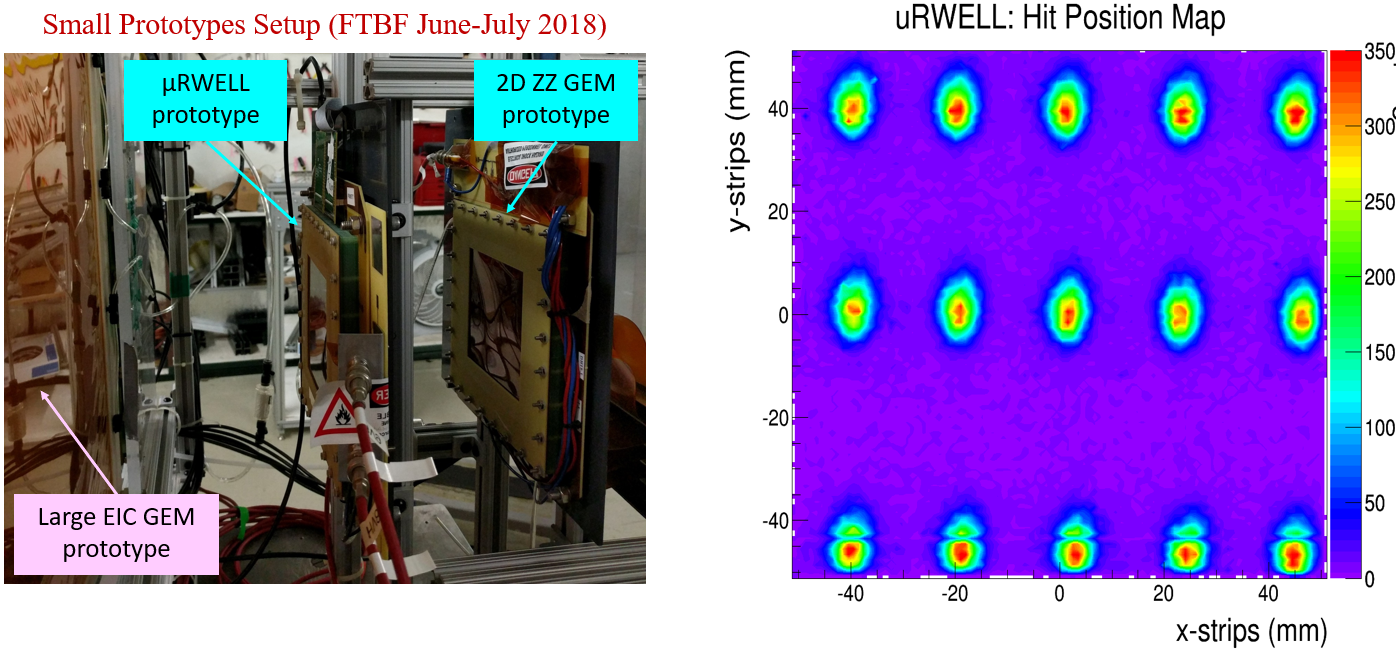
\includegraphics[width=1\columnwidth,trim={0pt 0mm 0pt 0mm},clip]{UVa_plots/ftbfSmallSetup}
\caption{\label{fig:ftbfSmallSetup} ({\it Left:}) Setup of $\mu$RWELL  prototype and a small triple-GEM prototype with 2D zigzag strip readout at the FTBF in June-July 2018. The prototypes were installed on the same moving table behind the large EIC GEM; ({\it Left:}) Reconstruction of the proton beam 2D spot from position scan run with the small prototypes}
\end{figure}
%
In addition, we also had a second detector configuration setup dedicated to a short study (one day beam time) of the small  $\mu$RWELL and the 2D zigzag GEM prototypes. In this second setup, the two small detectors were installed on the X-Y moving table behind the large EIC prototype as shown on Fig.~\ref{fig:ftbfSmallSetup}.\\
%
\begin{figure}[htb]
\centering
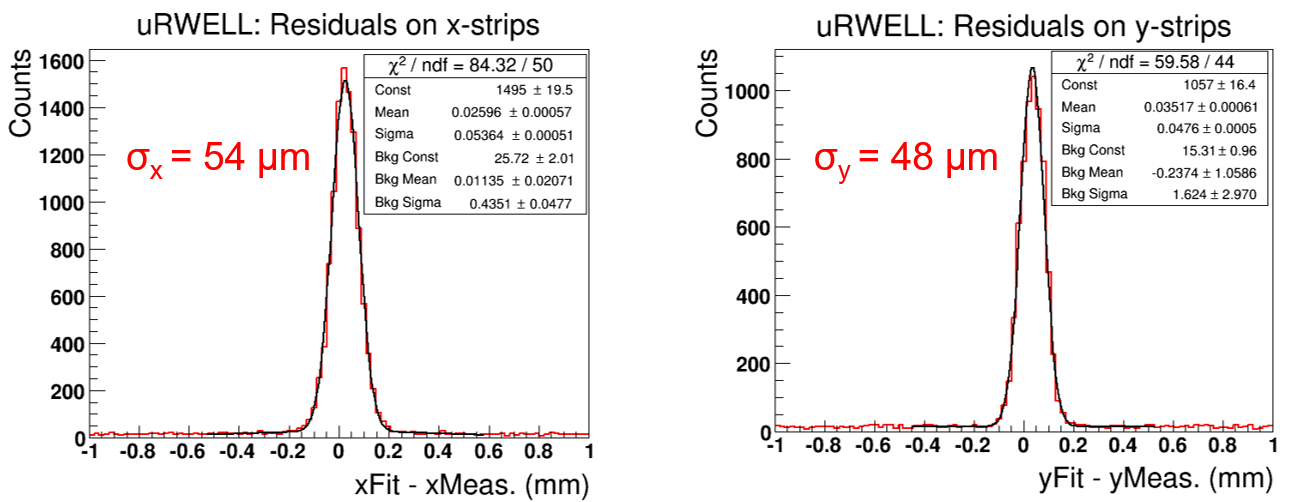
\includegraphics[width=1\columnwidth,trim={0pt 0mm 0pt 0mm},clip]{UVa_plots/uRwellResidual}
\caption{\label{fig:uRwellResidual} Residuals in x and y of the $\mu$RWELL prototype with the 120 GeV FTBF proton beam.}
\end{figure}
%

\subsubsection{Yale University} 

%
\subsection{What was not achieved, why not and what will be done to correct?} 
\subsubsection{Brookhaven National Lab} 
We have not yet measured the TPC prototype equipped with the Micromegas or micro-RWELL readouts since we've only fairly recently completed the assembly of the prototype equipped with GEMs and have not yet finished the measurements with this setup. However, we have recently received two zigzag PCB's, one coupled to a Micromegas, and the other coupled to a micro-RWELL. Preliminary testing of these boards has begun with further comissioning tests in planar detector configurations to follolw, before these boards are studied in the TPC prototype. In addition, we have not yet read out the TPC prototype with either the SAMPA or DREAM electronics mainly since the setup is new, but more so due to the fact that further work is required to read out these electronics through our data acquisition software.      
\subsubsection{Florida Tech} 
We have mostly achieved the goals that we had set for ourselves for the reporting period. There is some delay in the quality control tests for the low-mass prototype since the preparation for the assembly took a bit longer than expected.
\subsubsection{INFN Trieste} 
The activity is progressing according to  planning.
Nevertheless, the milestone: "September 2018: 
The performance of the tests to establish 
the compatibility of the ND photocathodes
with the operation of MPGD-based photon detectors."
could not be fully achieved. Some puzzling aspects 
of the performance observed using THGEM
with ND photocathode require repeated exercises
of production and test before reaching final conclusions.
\subsubsection{Stony Brook University} 
The completion of the evaporator setup is yet to be completed as the construction of the TPC-prototype took away significant time.
\subsubsection{Temple University} 
TU has not yet completed all of its goals for this current funding cycle. In regards to the hardware side, we have our third of four commercial triple-GEM detectors fully assembled, however we have not yet had time to start to fully characterize it (via cosmics/$^{55}$Fe). We also did not fully assemble the fourth and final commercial triple-GEM detector yet, because we wanted to wait until we tested the third GEM detector first, in case any alterations to the assembly process needed to be made. With the successful test of the third commercial triple-GEM detector, we are now ready to complete the assembly of the forth commercial triple-GEM detector. This will then be followed by testing and characterization of the detector.

TU also has not yet implemented a realistic digitization for the cylindrical shell MPGD operating in a $\mu$TPC mode, which prevents a realistic assessment of the tracking performance. This will be the main simulation focus of the remaining funding cycle.


\subsubsection{University of Virginia}
We have not started working on he design of Small cylindrical $\mu$RWELL prototype. We have so far concentrated our effort on the FTBF2018 test beam data analysis.
\\ We have not yet procure the small size VMM-based Scalable Readout System (SRS). We are waiting for the release of the final and stable  version of the VMM-SRS front end cards as well as the other boards of the readout system to place the order.
\\ The drafting of the publication paper on the Chromium GEM (Cr-GEM)  has been going slowly as we are concentration our efforts on other activities.
\subsubsection{Yale University} 


\section{Future}
\subsection[What is planned for the next funding cycle and beyond?]{What is planned for the next funding cycle and beyond? How, if at all, is this planning different from the original plan?}
\subsubsection{Brookhaven National Lab} 

Our proposed R\&D activity for the next funding cycle is as follows:

\begin{itemize}

\item Tests with TPC prototype (study track reconstruction using cosmic rays ) 
\item Study track reconstruction in TPC prototype in the lab using cosmic ray telescope (position resolution, Neff) 
\item TPC electronics (SAMPA, DREAM)
\item Continue work on optimizing the production of zigzag readouts in parallel with the eRD6 R\&D program 
\end{itemize}

General goals for the future

\begin{itemize}
\item Tests with TPC prototype (try different zigzag readout patterns; different avalanche schemes; gas choice; charge spread, attachment, and IBF measurements) 
\item Start work on simulation studies of the response of various zigzag readout patterns in combination with different detector gases and avalanche technologies.  
\item Study production of "laser tracks" in TPC drift region using our UV laser to ionize gas.

\end{itemize}

These plans are well aligned with our initial goals for this time period.
\subsubsection{Florida Tech} 
\begin{enumerate}
\item \textbf{Forward Tracker Prototype:} Our main goal for the next funding period is to extract the performance characteristics of the low-mass prototype from the data that we are hopefully about to collect at the Fermilab beam test and to present the results at conferences and in a publication. In addition, we will perform additional measurements on the detector with X-rays at Florida Tech, e.g.\ gain curves.
%
\item \textbf{EIC Simulations:} The next step in this study is to measure the track resolution of the electron track through the chambers. This will be implemented by adding a dummy plane about 15 cm past the third GEM ring. The simulated electron tracks will be focused on either the $x$ or $y$ axis, and the positions of events on the chosen axis will be histogrammed. In this fashion, one will be able to tell how the reduction of material in the GEM chambers affects the spread of position values read after the chambers due to multiple scattering. It is expected that the chromium configuration will produce a smaller spread than the standard configuration.
%
\item \textbf{$\mu$RWELL detector:} We plan to work closely with UVa on the design of a first prototype for a small cylindrical $\mu$RWELL detector. More details on this can be found in the proposal section below that describes the overall $\mu$RWELL detector R\&D that is proposed by the eRD6 consortium. Finally, we will assemble and commission the 10 $\times$ 10 cm$^2$ $\mu$RWELL prototype with zigzag-strip readout and characterise its performance using X-rays.
\end{enumerate}

 \subsubsection{INFN Trieste} 
 \label{sec:infn-planned-next}
For 2019, we confirm the planning that was presented in
June 2018 including two activities.
\begin{enumerate}
\item
\textbf{Single photon detector 
by MPGD technologies with 
miniaturized 
pad-size}. \\
The analysis of the data collected at the 2018 
test beam exercise where a first version of the 
prototype will be completed.\\
The realization and characterization by laboratory 
tests of a
second version of the prototype is also foreseen. 
The construction of this second version of the
prototype is 
related to the observed non-uniformity of the gain. 
As explained in the June 2018 report
the source of the effect has been understood:
it is related to the design of the anode PCB 
of the MM multiplication
stage. A modified version has already been designed. 
The construction and characterization 
of the modified prototype
will take place in 2019.
\item
\textbf{innovative photocathode 
based on NanoDiamond (ND) particles} \\
The initial studies to understand the 
compatibility of a photocathode 
based on NanoDiamond (ND) particles with the 
operation in gaseous detectors and, in 
particular, in MPGD-based photon detectors, 
have been performed in 2018. The characterization of
THGEMs with ND 
coating, both in the case of hydrogenated and
non-hydrogenated powder has presented unexpected
features, even if 
very different in the two cases.
The 2019 activity will be dedicated to further 
explore these 
performance in order to understand the origin of the
modified
THGEM behavior by producing under 
controlled parameters       a new set 
of small-size THGEMs, 
that then will be fully characterized.
\end{enumerate}
\par
Following the activity planning, the 
\textbf{milestones for 2019} are:
\begin{itemize}
\item
September 2019: The completion of the laboratory characterization 
of the second version of the photon detector with miniaturized pad-size.
\item
September 2019: The completion of the studies to understand the performance of THGEMs with ND coating, both in the hydrogenized and non-hydrogenized versions.
\end{itemize}
\subsubsection{Stony Brook University} 
The test-beam campaign at FTBF has been completed in the first week of July 2018 and the analysis of the TPC-prototype has been finalized. The results were presented at various internal meetings.\newline
We have acquired an X-ray tube setup with a gantry system that allows precisely controlled illumination of detectors with almost 

The installation of the evaporator equipment will be continued and first operation is expected in early fall.
\begin{itemize}
\item[-] Jan-Mar 2019 IBF measurements
\item[-] Jan-Apr 2019 final evaporation installation
\item[-] Apr-May 2019 evaporator commissioning
\end{itemize}
\subsubsection{Temple University} 
During the remaining time in this funding period, TU plans on finishing out the R\&D related to the commercial triple-GEM detectors. This includes assembling the triple-GEM stack of the fourth and last commercial GEM detector, and characterizing its performance along with the recently assembled third triple-GEM detector. The performance of both detectors will be assessed via cosmic and using an $^{55}$Fe source. This will complete the eRD3 carry over R\&D.

Additionally, TU will continue work on the simulating a MPGD cylindrical detector operating in a $\mu$TPC mode. In particular we will focus on implementing a realistic digitization scheme, which will be based on test beam results BNL acquired when testing a $\mu$TPC using a Compass readout. With the digitization scheme in place we can then assess accurate tracking performance of such a detector. Additionally we can then look at the tracking impact when including a TPC with the cylindrical MPGD shells, as well as integrating the forward MPGD tracking simulations that FIT is working on. This will allow us to study the global performance of the tracking detectors within the entire EIC phase space.   

\subsubsection{University of Virginia} 
Our plans and R\&D goals for next cycle of FY19 are:
%
\begin{enumerate}
%
\item \textbf{Large EIC-FT-GEM prototype:} Continue the analysis of the FTBF data. Present the results of the performances of the the prototype at MPGD2019 conferences in Spring 2019 and start preparing the draft for publication of these results in peer-reviewed journal.
%
\item \textbf{R\&D on $\mu$RWELL detector technology:} Continue the work on the design of a small cylindrical  $\mu$RWELL detector with FIT and TU. Procure a second 10 cm $\times$ 10 cm prototype with the R\&D focus on low mass and high resolution 2D readout strips patterns. We will also continue the study and characterization of our current small prototype and most importantly the performance of this new technology in high particle rate environment. 
%
\item \textbf{VMM readout Electronics:} Procure a small size VMM-based Scalable Readout System (SRS) if  a stable version of the FE cards are available and start testing this new  electronics with the our detectors to compare the performances of VMM-SRS readout system with the APV25 electronics.
%
\item \textbf{Draft paper on Chromium GEM (Cr-GEM) studies:}  Continue working on the draft  paper for the publication of the results in NIMA or TNS journal.
\end{enumerate}
\subsubsection{Yale University} 


\subsection{What are the critical issues?}
\subsubsection{Brookhaven National Lab} 
The most critical issue we wish to study is the performance of the various forms of readout in a TPC in an operating mode that is optimized for EIC. This is significantly different than what has been studied with these types of MPGDs and readout boards in eRD3/eRD6 in the past since the spatial resolution is affected by the diffusion of the primary ionization across the drift volume. One therefore wants to study the effect of this when used in combination with various forms of gas amplification devices and readout structures. In addition, the time resolution of the detector and the readout plays an important role as well, which is not so important in a simple planar detector. Finally, since the amount of ion feedback for a TPC operating at EIC will mostly likely be much less than for a TPC operating in a heavy ion environment such as sPHENIX and ALICE, the design of those TPCs will not necessarily be optimal for a TPC for EIC, and we would therefore like to determine the optimal design and operating conditions for the electron ion collider environment. 
\subsubsection{Florida Tech} 

\paragraph*{Technical Issues:} The original 3D-printed design of the pull-out posts for the low-mass detector proved to be not robust enough. Under tension force in the open detector, they tend to bend more than we expected and some show cracks. The original pull-out design is a copy of the pull-out used in the CMS forward muon GEM upgrade, but there the pull-outs are made from stainless steel whereas we attempted to use very light ABS material in the EIC prototype. We have changed the pull-out design to a solid block (Fig.~\ref{fig:Pullouts} left) that appears to be more stable. Some of the original pull-outs could be replaced with redesigned block pull-outs that are more robust before the beam test. At the time of the writing this report, the chamber is being retrofitted with additional pull-outs that are being 3D-printed at Fermilab. After the beam test, we plan to replace all pull-outs with new pull-outs made from aluminum or possibly PEEK.

\begin{figure}
	\centering
%		\includegraphics[width=8.2cm, height=6cm]{FIT_plots/Pullouts.JPG}
%		\includegraphics[width=8.2cm, height=6cm]{FIT_plots/Innerframes.JPG}
	\caption{\label{fig:Pullouts}Left: Comparison of original pull-out post (left) and redesigned pull-out post (right) that is more robust. Right: Gaps between inner frames on long sides (on right) cause some foil warping.}	
\end{figure}

On the long side of the detector, there are centimeter-wide gaps between the inner frames that cause some foil warping in those gaps (Fig.~\ref{fig:Pullouts} right). This in turn causes shorts between foils or HV instabilities as the distances between foils are not sufficiently constant. By contrast, the inner frames at the wide end of the trapezoid are very close to each other which keeps the foils smooth in that region. The gaps are the consequence of our original attempt to simplify the frame design by keeping all inner frame pieces at the same length. At the time of writing this report, we are retrofitting the chamber with longer inner frames on the sides that are being 3D-printed at Fermilab to close the gaps. Here we are taking advantage of the purely mechanical chamber construction method that allows a re-opening of the chamber.

\paragraph*{Manpower Issues:} The departure of our post-doc Aiwu Zhang back in December 2016 has severely slowed down progress. While our undergraduates are doing a great job and are very enthusiastic about building and testing prototype detectors and analyzing beam test data, they have limited availability and experience.

\subsubsection{INFN Trieste} 
No technical critical issue is expected 
for the completion of the
planed 2019 activity.
\par
Nevertheless, the exploratory exercises concerning the
photocathodes based on ND material can deserve surprises
related to the high innovative approach. The progress rate 
can be affected by these possible surprises.
\subsubsection{Stony Brook University} 
No critical issues have been identified.
\subsubsection{Temple University} 
No critical issues.
\subsubsection{University of Virginia}
No critical issues.
\subsubsection{Yale University} 

%
\subsection{Additional information}
\subsubsection{Brookhaven National Lab} 
None.
\subsubsection{Florida Tech} 
None.
\subsubsection{INFN Trieste} 
None.
\subsubsection{Stony Brook University} 
None.
\subsubsection{Temple University} 
None.
\subsubsection{University of Virginia} 
None.
\subsubsection{Yale University} 


\section{Manpower}
\subsection{Brookhaven National Lab} 
This work is being carried out by members of the BNL Physics Department. It includes two Senior Scientists (0.2 FTE), two Physics Associates (1.2 FTE), and one Technician (0.3 FTE). 
\subsection{Florida Tech} 

\begin{itemize}
\item Marcus Hohlmann, Professor, 0.25 FTE, not funded under this R\&D program.
\item Matthew Bomberger, physics undergraduate student, funded with \$1.7k in summer 2018 by this R\&D program.
\item Samantha Wohlstadter, physics undergraduate student, not funded.
\end{itemize}
\subsection{INFN Trieste} 
From INFN Trieste:
\begin {itemize}
\item C. Chatterjee (Trieste University and INFN, PhD student)
\item S. Dalla Torre (INFN, Staff)
\item S. Dasgupta (INFN, postdoc) 
\item S. Levorato (INFN, staff)
\item Triloki  (ICTP, postdoc)
\item F. Tessarotto (INFN, Staff)
\item Y. Zhao (INFN, postdoc)
\end{itemize}
The contribution of technical personnel from INFN-Trieste is also foreseen according to needs.
\par
From INFN BARI:
\begin {itemize}
\item Grazia Cicala (NCR staff and INFN)
\item Antonio Valentini (Bari University and INFN, professor)
\end{itemize}
\par
\textbf{Globally, the dedicated manpower is equivalent to 3 FTE.}
\subsection{Stony Brook University}
\begin{itemize}
\item K.~Dehmelt, Research Scientist, 0.3 FTE
\item T.~K.~Hemmick, Professor, 0.1 FTE
\item P.~Garg, Postdoc, 0.1 FTE
\end{itemize}
All personnel is not funded under this R\&D program.
\subsection{Temple University} 
Temple University's workforce is listed below:
\begin{itemize}
\item B. Surrow; Professor; 0.1 FTE
\item M. Posik; Assistant Research Professor; 0.2 FTE
\item A. Quintero; Post-doc ; 0.3 FTE
\end{itemize}
\subsection{University of Virginia} 
None of the labor at UVa is funded by EIC R\&D. The workforce is listed below:
\begin{itemize}
\item N. Liyanage; Professor; 0.1 FTE
\item K. Gnanvo; Research Scientist; 0.5 FTE
\end{itemize}
\subsection{Yale University} 


\section{External Funding}
\subsection{Brookhaven National Lab} 
All scientific manpower at BNL would be provided by internal funding. However, technician and designer labor would need to be supported through EIC R\&D funds.   

Additional work on R\&D on Micropattern Detectors for EIC is also being provided by a BNL LDRD in collaboration with Saclay and Stony Brook. This is supporting our continued work on zig-zag readout with GEMs and Micromegas and we do not request any funding for this effort from EID R\&D funds. However, our proposed work on TPC R\&D for EIC would not be covered under LDRD funds.

\subsection{Florida Tech} 
None.
\subsection{INFN Trieste}
INFN has assigned to this activity a support of 11.5 keuro 
for the year 2019.
\subsection{Stony Brook University} 
There is no external funding for this R\&D effort.
\subsection{Temple University} 
UVa has DOE basic research grant from Medium Energy Physics. The R\&D work on Cr-GEM is partly funded with the research grant.
\subsection{University of Virginia} 
UVa has DOE basic research grant from Medium Energy Physics. The R\&D work on Cr-GEM is partly funded with the research grant.
\subsection{Yale University} 


\printbibliography

%
% mlp -- the easiest to extract (and then trim) all enrtries in a given bib file is e.g.
%  grep @ BNL.bib | awk -F{ '{print $NF}'

\appendix
\section{List of all EIC publications from the eRD6 Consortium}
%
  \begin{refsection}
    \renewcommand{\refname}{BNL publications:}
    \nocite{8379440, 7497629, Woody:2015ola, 7431059, 6829463}
    \printbibliography
  \end{refsection}
%  
  \begin{refsection}
    \renewcommand{\refname}{Florida Tech publications:}
    \nocite{Hohlmann:2017sqj, Zhang:2017dqw, Zhang:2016vbk, Zhang:2015kxy, Zhang:2015pqa}
    \printbibliography
  \end{refsection}
%  
  \begin{refsection}
    \renewcommand{\refname}{INFN publications:}
     \nocite{AGARWALA2018-2, Agarwala:2018qdm}
     \printbibliography    
  \end{refsection}
%
  \begin{refsection}
    \renewcommand{\refname}{SBU publications:}
    \nocite{Blatnik:2015bka}
    \printbibliography    
  \end{refsection}
%  
  \begin{refsection}
    \renewcommand{\refname}{TU publications:}
    \nocite{Gnanvo:2014hpa, Gnanvo:2015xda}
    \printbibliography
  \end{refsection}
  %
  \begin{refsection}
    \renewcommand{\refname}{UVa publications:}
    \nocite{Gnanvo:2014hpa, Gnanvo:2015xda}
    \printbibliography
  \end{refsection}
%
  \begin{refsection}
    \renewcommand{\refname}{Yale publications:}
    \nocite{Aiola:2016rld}
    \printbibliography    
  \end{refsection}  
%  
\end{document}
